\documentclass[]{article}
\usepackage{lmodern}
\usepackage{amssymb,amsmath}
\usepackage{ifxetex,ifluatex}
\usepackage{fixltx2e} % provides \textsubscript
\ifnum 0\ifxetex 1\fi\ifluatex 1\fi=0 % if pdftex
  \usepackage[T1]{fontenc}
  \usepackage[utf8]{inputenc}
\else % if luatex or xelatex
  \ifxetex
    \usepackage{mathspec}
  \else
    \usepackage{fontspec}
  \fi
  \defaultfontfeatures{Ligatures=TeX,Scale=MatchLowercase}
\fi
% use upquote if available, for straight quotes in verbatim environments
\IfFileExists{upquote.sty}{\usepackage{upquote}}{}
% use microtype if available
\IfFileExists{microtype.sty}{%
\usepackage{microtype}
\UseMicrotypeSet[protrusion]{basicmath} % disable protrusion for tt fonts
}{}
\usepackage[margin=1in]{geometry}
\usepackage{hyperref}
\hypersetup{unicode=true,
            pdftitle={MAthesis},
            pdfborder={0 0 0},
            breaklinks=true}
\urlstyle{same}  % don't use monospace font for urls
\usepackage{color}
\usepackage{fancyvrb}
\newcommand{\VerbBar}{|}
\newcommand{\VERB}{\Verb[commandchars=\\\{\}]}
\DefineVerbatimEnvironment{Highlighting}{Verbatim}{commandchars=\\\{\}}
% Add ',fontsize=\small' for more characters per line
\usepackage{framed}
\definecolor{shadecolor}{RGB}{248,248,248}
\newenvironment{Shaded}{\begin{snugshade}}{\end{snugshade}}
\newcommand{\KeywordTok}[1]{\textcolor[rgb]{0.13,0.29,0.53}{\textbf{{#1}}}}
\newcommand{\DataTypeTok}[1]{\textcolor[rgb]{0.13,0.29,0.53}{{#1}}}
\newcommand{\DecValTok}[1]{\textcolor[rgb]{0.00,0.00,0.81}{{#1}}}
\newcommand{\BaseNTok}[1]{\textcolor[rgb]{0.00,0.00,0.81}{{#1}}}
\newcommand{\FloatTok}[1]{\textcolor[rgb]{0.00,0.00,0.81}{{#1}}}
\newcommand{\ConstantTok}[1]{\textcolor[rgb]{0.00,0.00,0.00}{{#1}}}
\newcommand{\CharTok}[1]{\textcolor[rgb]{0.31,0.60,0.02}{{#1}}}
\newcommand{\SpecialCharTok}[1]{\textcolor[rgb]{0.00,0.00,0.00}{{#1}}}
\newcommand{\StringTok}[1]{\textcolor[rgb]{0.31,0.60,0.02}{{#1}}}
\newcommand{\VerbatimStringTok}[1]{\textcolor[rgb]{0.31,0.60,0.02}{{#1}}}
\newcommand{\SpecialStringTok}[1]{\textcolor[rgb]{0.31,0.60,0.02}{{#1}}}
\newcommand{\ImportTok}[1]{{#1}}
\newcommand{\CommentTok}[1]{\textcolor[rgb]{0.56,0.35,0.01}{\textit{{#1}}}}
\newcommand{\DocumentationTok}[1]{\textcolor[rgb]{0.56,0.35,0.01}{\textbf{\textit{{#1}}}}}
\newcommand{\AnnotationTok}[1]{\textcolor[rgb]{0.56,0.35,0.01}{\textbf{\textit{{#1}}}}}
\newcommand{\CommentVarTok}[1]{\textcolor[rgb]{0.56,0.35,0.01}{\textbf{\textit{{#1}}}}}
\newcommand{\OtherTok}[1]{\textcolor[rgb]{0.56,0.35,0.01}{{#1}}}
\newcommand{\FunctionTok}[1]{\textcolor[rgb]{0.00,0.00,0.00}{{#1}}}
\newcommand{\VariableTok}[1]{\textcolor[rgb]{0.00,0.00,0.00}{{#1}}}
\newcommand{\ControlFlowTok}[1]{\textcolor[rgb]{0.13,0.29,0.53}{\textbf{{#1}}}}
\newcommand{\OperatorTok}[1]{\textcolor[rgb]{0.81,0.36,0.00}{\textbf{{#1}}}}
\newcommand{\BuiltInTok}[1]{{#1}}
\newcommand{\ExtensionTok}[1]{{#1}}
\newcommand{\PreprocessorTok}[1]{\textcolor[rgb]{0.56,0.35,0.01}{\textit{{#1}}}}
\newcommand{\AttributeTok}[1]{\textcolor[rgb]{0.77,0.63,0.00}{{#1}}}
\newcommand{\RegionMarkerTok}[1]{{#1}}
\newcommand{\InformationTok}[1]{\textcolor[rgb]{0.56,0.35,0.01}{\textbf{\textit{{#1}}}}}
\newcommand{\WarningTok}[1]{\textcolor[rgb]{0.56,0.35,0.01}{\textbf{\textit{{#1}}}}}
\newcommand{\AlertTok}[1]{\textcolor[rgb]{0.94,0.16,0.16}{{#1}}}
\newcommand{\ErrorTok}[1]{\textcolor[rgb]{0.64,0.00,0.00}{\textbf{{#1}}}}
\newcommand{\NormalTok}[1]{{#1}}
\usepackage{longtable,booktabs}
\usepackage{graphicx,grffile}
\makeatletter
\def\maxwidth{\ifdim\Gin@nat@width>\linewidth\linewidth\else\Gin@nat@width\fi}
\def\maxheight{\ifdim\Gin@nat@height>\textheight\textheight\else\Gin@nat@height\fi}
\makeatother
% Scale images if necessary, so that they will not overflow the page
% margins by default, and it is still possible to overwrite the defaults
% using explicit options in \includegraphics[width, height, ...]{}
\setkeys{Gin}{width=\maxwidth,height=\maxheight,keepaspectratio}
\IfFileExists{parskip.sty}{%
\usepackage{parskip}
}{% else
\setlength{\parindent}{0pt}
\setlength{\parskip}{6pt plus 2pt minus 1pt}
}
\setlength{\emergencystretch}{3em}  % prevent overfull lines
\providecommand{\tightlist}{%
  \setlength{\itemsep}{0pt}\setlength{\parskip}{0pt}}
\setcounter{secnumdepth}{0}
% Redefines (sub)paragraphs to behave more like sections
\ifx\paragraph\undefined\else
\let\oldparagraph\paragraph
\renewcommand{\paragraph}[1]{\oldparagraph{#1}\mbox{}}
\fi
\ifx\subparagraph\undefined\else
\let\oldsubparagraph\subparagraph
\renewcommand{\subparagraph}[1]{\oldsubparagraph{#1}\mbox{}}
\fi

%%% Use protect on footnotes to avoid problems with footnotes in titles
\let\rmarkdownfootnote\footnote%
\def\footnote{\protect\rmarkdownfootnote}

%%% Change title format to be more compact
\usepackage{titling}

% Create subtitle command for use in maketitle
\newcommand{\subtitle}[1]{
  \posttitle{
    \begin{center}\large#1\end{center}
    }
}

\setlength{\droptitle}{-2em}
  \title{MAthesis}
  \pretitle{\vspace{\droptitle}\centering\huge}
  \posttitle{\par}
  \author{}
  \preauthor{}\postauthor{}
  \date{}
  \predate{}\postdate{}

\usepackage{setspace}
\doublespacing

\begin{document}
\maketitle

{
\setcounter{tocdepth}{2}
\tableofcontents
}
\section{Time bins (stratigraphic
stages)}\label{time-bins-stratigraphic-stages}

\begin{longtable}[]{@{}lllrrrr@{}}
\caption{Smaller time bins with age range, epoch name, mean age and
corresponding sample sizes (on individual, species and genus
level)}\tabularnewline
\toprule
bin & EpochBins & Stages & MeanBins & nIndividuals & nSpecies &
nGenera\tabularnewline
\midrule
\endfirsthead
\toprule
bin & EpochBins & Stages & MeanBins & nIndividuals & nSpecies &
nGenera\tabularnewline
\midrule
\endhead
(0,0.0117{]} & Modern & Modern & 0.00585 & 253 & 65 & 18\tabularnewline
(0.0117,0.126{]} & Upper Pleistocene & Upper Pleistocene & 0.06885 & 49
& 18 & 8\tabularnewline
(0.126,0.781{]} & Middle Pleistocene & Middle Pleistocene & 0.45350 & 53
& 13 & 7\tabularnewline
(0.781,1.81{]} & Lower Pleistocene & Lower Pleistocene & 1.29350 & 57 &
27 & 12\tabularnewline
(1.81,2.59{]} & Gelasian & Lower Pleistocene & 2.19700 & 31 & 14 &
8\tabularnewline
(2.59,3.6{]} & Piacencian & Upper Pliocene & 3.09400 & 21 & 14 &
9\tabularnewline
(3.6,5.33{]} & Zanclean & Lower Pliocene & 4.46600 & 26 & 14 &
8\tabularnewline
(5.33,7.25{]} & Messinian & Upper Miocene & 6.28900 & 10 & 7 &
4\tabularnewline
(7.25,11.6{]} & Tortonian & Upper Miocene & 9.42700 & 45 & 20 &
9\tabularnewline
(11.6,13.8{]} & Serravallian & Middle Miocene & 12.71400 & 27 & 8 &
6\tabularnewline
(13.8,16{]} & Langhian & Middle Miocene & 14.89500 & 14 & 10 &
7\tabularnewline
(16,23{]} & Burdigalian/Aquitanian & Lower Miocene & 19.50000 & 30 & 14
& 9\tabularnewline
\bottomrule
\end{longtable}

\begin{figure}[htbp]
\centering
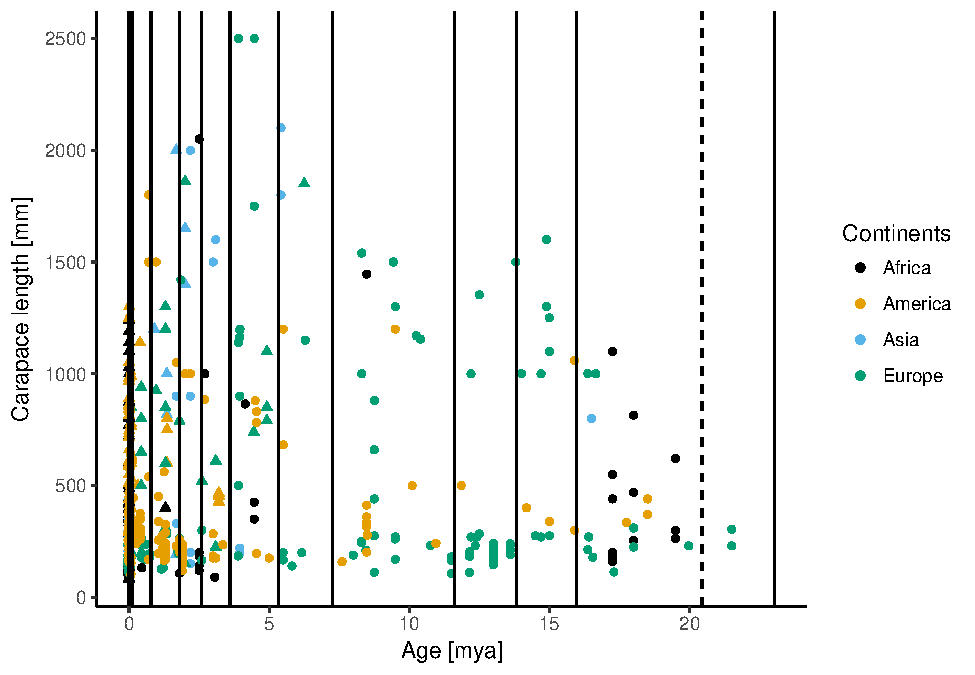
\includegraphics{MA_JJ_files/figure-latex/overviewData-1.pdf}
\caption{Scatterplot of carapace length over time, indicating insular
(triangle) and continental (circles) and colour indicating continents.
Lines indicate stratigraphic stages which were used as time bins, the
dashed line is the border between the two stages of the Lower Miocene,
which were consideres as one time bin.}
\end{figure}

\newpage

\section{Maps}\label{maps}

\subsection{fossil occurences of
testudinidae}\label{fossil-occurences-of-testudinidae}

\begin{verbatim}
## [1] 193
\end{verbatim}

\begin{figure}[htbp]
\centering
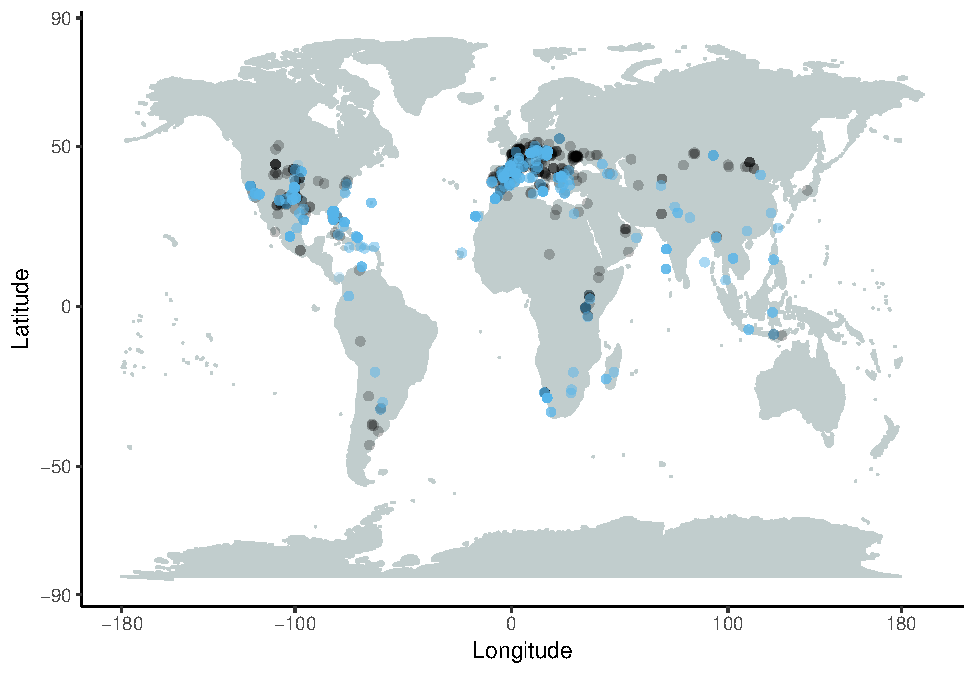
\includegraphics{MA_JJ_files/figure-latex/MapFossilOccurrences-1.pdf}
\caption{Map displaying all fossil occurrences of testudinids, with
color indicating whether relevant literature was available (black if
not) and if it was, whether body size data was available or not (yes and
no, respectively).}
\end{figure}

\newpage

\subsection{body size of testudinidae}\label{body-size-of-testudinidae}

\begin{figure}[htbp]
\centering
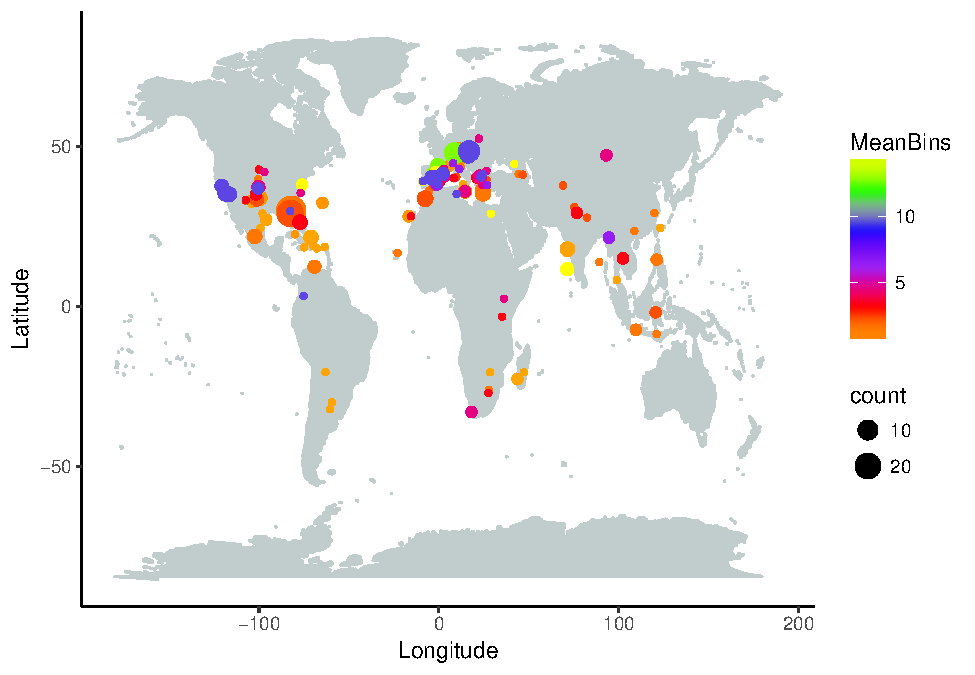
\includegraphics{MA_JJ_files/figure-latex/MapCL-1.pdf}
\caption{Map displaying all localities for which body size data for
testudinids was available in the literature. Size of points denotes
sample size, color denotes approximate age.}
\end{figure}

\begin{longtable}[]{@{}llrr@{}}
\caption{Overview over fossil species per time bin, with sample size and
mean CL.}\tabularnewline
\toprule
EpochBins & Taxon & n & meanCL\tabularnewline
\midrule
\endfirsthead
\toprule
EpochBins & Taxon & n & meanCL\tabularnewline
\midrule
\endhead
Upper Pleistocene & Centrochelys robusta & 1 & 850.0000\tabularnewline
Upper Pleistocene & Chelonoidis denticulata & 1 &
616.0000\tabularnewline
Upper Pleistocene & Chelonoidis lutzae & 1 & 830.0000\tabularnewline
Upper Pleistocene & Chelonoidis marcanoi & 4 & 672.2500\tabularnewline
Upper Pleistocene & Chelonoidis monensis & 1 & 500.0000\tabularnewline
Upper Pleistocene & Chelonoidis sombrerensis & 1 &
990.0000\tabularnewline
Upper Pleistocene & Chelonoidis sp. & 3 & 666.6667\tabularnewline
Upper Pleistocene & Eurotestudo hermanni & 1 & 187.0000\tabularnewline
Upper Pleistocene & gen. indet. & 1 & 813.0000\tabularnewline
Upper Pleistocene & Geochelone sp. & 2 & 475.0000\tabularnewline
Upper Pleistocene & Gopherus agassizi & 1 & 252.0000\tabularnewline
Upper Pleistocene & Gopherus polyphemus & 20 & 292.9700\tabularnewline
Upper Pleistocene & Gopherus praecedens & 1 & 360.0000\tabularnewline
Upper Pleistocene & Hesperotestudo crassiscutata & 6 &
435.1667\tabularnewline
Upper Pleistocene & Hesperotestudo incisa & 1 & 232.7600\tabularnewline
Upper Pleistocene & Hesperotestudo sp. & 2 & 806.5000\tabularnewline
Upper Pleistocene & Hesperotestudo wilsoni & 1 & 226.0000\tabularnewline
Upper Pleistocene & Indotestudo elongata & 1 & 270.0000\tabularnewline
Middle Pleistocene & Centrochelys burchardi & 4 &
722.5000\tabularnewline
Middle Pleistocene & Chelonoidis cubensis & 1 & 1139.0000\tabularnewline
Middle Pleistocene & Eurotestudo aff. hermanni & 2 &
187.0000\tabularnewline
Middle Pleistocene & Eurotestudo hermanni & 2 & 204.0500\tabularnewline
Middle Pleistocene & Geochelone sp. & 1 & 170.0000\tabularnewline
Middle Pleistocene & Gopherus agassizi & 1 & 445.0000\tabularnewline
Middle Pleistocene & Gopherus laticaudatus & 1 & 375.0000\tabularnewline
Middle Pleistocene & Gopherus polyphemus & 31 & 300.4316\tabularnewline
Middle Pleistocene & Hesperotestudo bermudae & 2 &
385.0000\tabularnewline
Middle Pleistocene & Hesperotestudo equicomes & 1 &
340.0000\tabularnewline
Middle Pleistocene & Hesperotestudo sp. & 2 & 1650.0000\tabularnewline
Middle Pleistocene & Testudo kenitrensis & 1 & 132.0000\tabularnewline
Middle Pleistocene & Testudo lunellensis & 4 & 215.4250\tabularnewline
Lower Pleistocene & Centrochelys atlantica & 1 & 400.0000\tabularnewline
Lower Pleistocene & Centrochelys robusta & 3 & 883.3333\tabularnewline
Lower Pleistocene & Cheirogaster cf.~gymnesica & 1 &
789.0000\tabularnewline
Lower Pleistocene & Cheirogaster sp. & 1 & 925.0000\tabularnewline
Lower Pleistocene & Chelonoidis sp. & 3 & 716.6667\tabularnewline
Lower Pleistocene & Eurotestudo globosa & 1 & 263.0000\tabularnewline
Lower Pleistocene & Eurotestudo hermanni & 2 & 205.0000\tabularnewline
Lower Pleistocene & gen. indet. & 1 & 900.0000\tabularnewline
Lower Pleistocene & Geochelone sp. & 1 & 340.0000\tabularnewline
Lower Pleistocene & Gopherus berlandieri & 2 & 225.6500\tabularnewline
Lower Pleistocene & Gopherus flavomarginatus & 1 &
450.0000\tabularnewline
Lower Pleistocene & Gopherus pertenuis & 1 & 1050.0000\tabularnewline
Lower Pleistocene & Gopherus polyphemus & 3 & 254.4667\tabularnewline
Lower Pleistocene & Gopherus sp. & 6 & 233.9667\tabularnewline
Lower Pleistocene & Hesperotestudo crassiscutata & 5 &
285.6000\tabularnewline
Lower Pleistocene & Hesperotestudo incisa & 7 & 234.6286\tabularnewline
Lower Pleistocene & Hesperotestudo mlynarskii & 2 &
184.2500\tabularnewline
Lower Pleistocene & Hesperotestudo sp. & 1 & 1500.0000\tabularnewline
Lower Pleistocene & Hesperotestudo turgida & 1 & 230.0000\tabularnewline
Lower Pleistocene & Megalochelys sondaari & 2 & 909.0000\tabularnewline
Lower Pleistocene & Megalochelys sp. & 3 & 1130.4667\tabularnewline
Lower Pleistocene & Psammobates antiquorum & 1 & 107.8000\tabularnewline
Lower Pleistocene & Testudo changshanesis & 1 & 330.0000\tabularnewline
Lower Pleistocene & Testudo graeca & 1 & 195.0000\tabularnewline
Lower Pleistocene & Testudo hermanni & 2 & 176.5500\tabularnewline
Lower Pleistocene & Testudo marginata & 3 & 270.0000\tabularnewline
Lower Pleistocene & Titanochelon gymnesica & 1 &
1300.0000\tabularnewline
Gelasian & Centrochelys marocana & 1 & 2050.0000\tabularnewline
Gelasian & Eurotestudo cf.~hermanni & 1 & 150.0000\tabularnewline
Gelasian & Gopherus sp. & 15 & 185.7467\tabularnewline
Gelasian & Hesperotestudo campester & 1 & 1000.0000\tabularnewline
Gelasian & Hesperotestudo sp. & 1 & 1000.0000\tabularnewline
Gelasian & Manouria punjabiensis & 1 & 900.0000\tabularnewline
Gelasian & Megalochelys atlas & 3 & 1683.3333\tabularnewline
Gelasian & Testudo aff. kenitrensis & 1 & 142.0000\tabularnewline
Gelasian & Testudo oughlamensis & 1 & 120.0000\tabularnewline
Gelasian & Testudo ranovi & 1 & 200.0000\tabularnewline
Gelasian & Testudo sp. & 2 & 192.0000\tabularnewline
Gelasian & Testudo transcaucasia & 1 & 150.0000\tabularnewline
Gelasian & Titanochelon aff. schafferi & 1 & 1860.0000\tabularnewline
Gelasian & Titanochelon sp. & 1 & 1420.0000\tabularnewline
Piacencian & ``Aldabrachelys'' laetoliensis & 1 &
1000.0000\tabularnewline
Piacencian & Aldabrachelys ? sp. & 2 & 1500.0000\tabularnewline
Piacencian & Centrochelys vulcanica & 1 & 610.0000\tabularnewline
Piacencian & Chelonoidis alburyorum & 4 & 442.7500\tabularnewline
Piacencian & Gopherus canyonensis & 1 & 885.5000\tabularnewline
Piacencian & Hesperotestudo johnstoni & 1 & 235.0000\tabularnewline
Piacencian & Hesperotestudo oelrichi & 1 & 283.8000\tabularnewline
Piacencian & Hesperotestudo riggsi & 2 & 180.5000\tabularnewline
Piacencian & Hesperotestudo sp. & 1 & 176.0000\tabularnewline
Piacencian & Homopus fenestratus & 1 & 90.0000\tabularnewline
Piacencian & Megalochelys atlas & 2 & 1600.0000\tabularnewline
Piacencian & Testudo brevitesta & 2 & 232.5000\tabularnewline
Piacencian & Testudo pecorinii & 1 & 225.0000\tabularnewline
Piacencian & Titanochelon sp. & 1 & 520.0000\tabularnewline
Zanclean & Caudochelys rexroadensis & 2 & 805.5000\tabularnewline
Zanclean & Centrochelys robusta & 3 & 913.3333\tabularnewline
Zanclean & Cheirogaster gymnesica & 1 & 739.0000\tabularnewline
Zanclean & Ergilemys oskarkuhni & 2 & 209.0000\tabularnewline
Zanclean & Geochelone crassa & 1 & 865.0000\tabularnewline
Zanclean & Geochelone s. l. & 1 & 1750.0000\tabularnewline
Zanclean & Geochelone sp. & 2 & 528.0000\tabularnewline
Zanclean & Geochelone stromeri & 2 & 387.5000\tabularnewline
Zanclean & Hesperotestudo riggsi & 1 & 195.8000\tabularnewline
Zanclean & Testudo cf.~graeca & 1 & 185.0000\tabularnewline
Zanclean & Testudo sp. & 4 & 1675.0000\tabularnewline
Zanclean & Titanochelon bacharidisi & 4 & 1040.0000\tabularnewline
Zanclean & Titanochelon perpiniana & 1 & 1140.0000\tabularnewline
Zanclean & Titanochelon schafferi & 1 & 2500.0000\tabularnewline
Messinian & Hesperotestudo orthopygia & 2 & 941.0000\tabularnewline
Messinian & Megalochelys atlas & 2 & 1950.0000\tabularnewline
Messinian & Testudo amiatae & 1 & 140.0000\tabularnewline
Messinian & Testudo graeca & 2 & 183.5000\tabularnewline
Messinian & Testudo sp. & 1 & 200.0000\tabularnewline
Messinian & Titanochelon bolivari & 1 & 1150.0000\tabularnewline
Messinian & Titanochelon schafferi & 1 & 1850.0000\tabularnewline
Tortonian & ``Hadrianus sp.'' & 1 & 1000.0000\tabularnewline
Tortonian & Cheirogaster richardi & 1 & 1155.0000\tabularnewline
Tortonian & Cheirogaster sp. & 2 & 1355.0000\tabularnewline
Tortonian & gen. indet. & 3 & 660.0000\tabularnewline
Tortonian & Geochelone hesterna & 1 & 278.0000\tabularnewline
Tortonian & Geochelone sp. & 2 & 973.0000\tabularnewline
Tortonian & Gopherus ? sp. & 1 & 500.0000\tabularnewline
Tortonian & Gopherus mohavetus & 5 & 324.8000\tabularnewline
Tortonian & Hesperotestudo alleni & 1 & 240.9000\tabularnewline
Tortonian & Hesperotestudo riggsi & 2 & 159.5000\tabularnewline
Tortonian & Hesperotestudo sp. & 1 & 1200.0000\tabularnewline
Tortonian & Paleotestudo sp. & 3 & 233.6667\tabularnewline
Tortonian & Testudo burgenlandica & 2 & 193.5000\tabularnewline
Tortonian & Testudo catalaunica & 4 & 157.0000\tabularnewline
Tortonian & Testudo cf.~promarginata & 5 & 250.0000\tabularnewline
Tortonian & Testudo graeca & 1 & 210.0000\tabularnewline
Tortonian & Testudo s. s. & 1 & 189.0000\tabularnewline
Tortonian & Testudo sp. & 7 & 243.1571\tabularnewline
Tortonian & Titanochelon bolivari & 1 & 1300.0000\tabularnewline
Tortonian & Titanochelon cf.~bolivari & 1 & 1500.0000\tabularnewline
Serravallian & Cheirogaster sp. & 2 & 1250.0000\tabularnewline
Serravallian & gen. indet. & 1 & 270.0000\tabularnewline
Serravallian & Gopherus ? sp. & 1 & 500.0000\tabularnewline
Serravallian & Paleotestudo antiqua & 18 & 203.0556\tabularnewline
Serravallian & Paleotestudo cf.~sp. & 1 & 270.0000\tabularnewline
Serravallian & Testudo catalaunica & 1 & 232.0000\tabularnewline
Serravallian & Testudo steinheimensis & 2 & 169.3500\tabularnewline
Serravallian & Titanochelon bolivari & 1 & 1353.0000\tabularnewline
Langhian & Caudochelys ducateli & 1 & 339.9000\tabularnewline
Langhian & Chelonoidis sp. & 3 & 553.3333\tabularnewline
Langhian & Ergilemys sp. & 1 & 1000.0000\tabularnewline
Langhian & gen. indet. & 1 & 1000.0000\tabularnewline
Langhian & Paleotestudo antiqua & 1 & 275.0000\tabularnewline
Langhian & Paleotestudo cf.~sp. & 1 & 270.0000\tabularnewline
Langhian & Testudo kalksburgensis & 1 & 275.0000\tabularnewline
Langhian & Testudo sp. & 1 & 400.0000\tabularnewline
Langhian & Titanochelon bolivari & 2 & 1175.0000\tabularnewline
Langhian & Titanochelon cf.~bolivari & 2 & 1450.0000\tabularnewline
Burdigalian/Aquitanian & Caudochelys williamsi & 1 &
334.0000\tabularnewline
Burdigalian/Aquitanian & gen. indet. & 1 & 270.0000\tabularnewline
Burdigalian/Aquitanian & Geochelone sp. & 2 & 900.0000\tabularnewline
Burdigalian/Aquitanian & Geochelone tedwhitei & 2 &
405.0000\tabularnewline
Burdigalian/Aquitanian & Impregnochelys pachytectis & 1 &
620.0000\tabularnewline
Burdigalian/Aquitanian & Mesocherus orangeus & 5 &
180.0000\tabularnewline
Burdigalian/Aquitanian & Namibchersus aff. namaquensis & 3 &
696.6667\tabularnewline
Burdigalian/Aquitanian & Namibchersus namaquensis & 6 &
428.8333\tabularnewline
Burdigalian/Aquitanian & Paleotestudo cf.~antiqua & 1 &
113.0000\tabularnewline
Burdigalian/Aquitanian & Paleotestudo sp. & 1 & 179.3000\tabularnewline
Burdigalian/Aquitanian & Testudo kalksburgensis & 2 &
227.5000\tabularnewline
Burdigalian/Aquitanian & Testudo promarginata & 3 &
281.5667\tabularnewline
Burdigalian/Aquitanian & Testudo rectogularis & 1 &
213.0000\tabularnewline
Burdigalian/Aquitanian & Titanochelon cf.~perpiniana & 1 &
1001.0000\tabularnewline
\bottomrule
\end{longtable}

\begin{longtable}[]{@{}lrr@{}}
\caption{General overview over fossil species, with sample size and mean
CL}\tabularnewline
\toprule
Taxon & n & meanCL\tabularnewline
\midrule
\endfirsthead
\toprule
Taxon & n & meanCL\tabularnewline
\midrule
\endhead
``Aldabrachelys'' laetoliensis & 1 & 1000.0000\tabularnewline
``Hadrianus sp.'' & 1 & 1000.0000\tabularnewline
Aldabrachelys ? sp. & 2 & 1500.0000\tabularnewline
Caudochelys ducateli & 1 & 339.9000\tabularnewline
Caudochelys rexroadensis & 2 & 805.5000\tabularnewline
Caudochelys williamsi & 1 & 334.0000\tabularnewline
Centrochelys atlantica & 1 & 400.0000\tabularnewline
Centrochelys burchardi & 4 & 722.5000\tabularnewline
Centrochelys marocana & 1 & 2050.0000\tabularnewline
Centrochelys robusta & 7 & 891.4286\tabularnewline
Centrochelys vulcanica & 1 & 610.0000\tabularnewline
Cheirogaster cf.~gymnesica & 1 & 789.0000\tabularnewline
Cheirogaster gymnesica & 1 & 739.0000\tabularnewline
Cheirogaster richardi & 1 & 1155.0000\tabularnewline
Cheirogaster sp. & 5 & 1227.0000\tabularnewline
Chelonoidis alburyorum & 4 & 442.7500\tabularnewline
Chelonoidis cubensis & 1 & 1139.0000\tabularnewline
Chelonoidis denticulata & 1 & 616.0000\tabularnewline
Chelonoidis lutzae & 1 & 830.0000\tabularnewline
Chelonoidis marcanoi & 4 & 672.2500\tabularnewline
Chelonoidis monensis & 1 & 500.0000\tabularnewline
Chelonoidis sombrerensis & 1 & 990.0000\tabularnewline
Chelonoidis sp. & 9 & 645.5556\tabularnewline
Ergilemys oskarkuhni & 2 & 209.0000\tabularnewline
Ergilemys sp. & 1 & 1000.0000\tabularnewline
Eurotestudo aff. hermanni & 2 & 187.0000\tabularnewline
Eurotestudo cf.~hermanni & 1 & 150.0000\tabularnewline
Eurotestudo globosa & 1 & 263.0000\tabularnewline
Eurotestudo hermanni & 5 & 201.0200\tabularnewline
gen. indet. & 8 & 654.1250\tabularnewline
Geochelone crassa & 1 & 865.0000\tabularnewline
Geochelone hesterna & 1 & 278.0000\tabularnewline
Geochelone s. l. & 1 & 1750.0000\tabularnewline
Geochelone sp. & 10 & 626.2000\tabularnewline
Geochelone stromeri & 2 & 387.5000\tabularnewline
Geochelone tedwhitei & 2 & 405.0000\tabularnewline
Gopherus ? sp. & 2 & 500.0000\tabularnewline
Gopherus agassizi & 2 & 348.5000\tabularnewline
Gopherus berlandieri & 2 & 225.6500\tabularnewline
Gopherus canyonensis & 1 & 885.5000\tabularnewline
Gopherus flavomarginatus & 1 & 450.0000\tabularnewline
Gopherus laticaudatus & 1 & 375.0000\tabularnewline
Gopherus mohavetus & 5 & 324.8000\tabularnewline
Gopherus pertenuis & 1 & 1050.0000\tabularnewline
Gopherus polyphemus & 54 & 295.1144\tabularnewline
Gopherus praecedens & 1 & 360.0000\tabularnewline
Gopherus sp. & 21 & 199.5238\tabularnewline
Hesperotestudo alleni & 1 & 240.9000\tabularnewline
Hesperotestudo bermudae & 2 & 385.0000\tabularnewline
Hesperotestudo campester & 1 & 1000.0000\tabularnewline
Hesperotestudo crassiscutata & 11 & 367.1818\tabularnewline
Hesperotestudo equicomes & 1 & 340.0000\tabularnewline
Hesperotestudo incisa & 8 & 234.3950\tabularnewline
Hesperotestudo johnstoni & 1 & 235.0000\tabularnewline
Hesperotestudo mlynarskii & 2 & 184.2500\tabularnewline
Hesperotestudo oelrichi & 1 & 283.8000\tabularnewline
Hesperotestudo orthopygia & 2 & 941.0000\tabularnewline
Hesperotestudo riggsi & 5 & 175.1600\tabularnewline
Hesperotestudo sp. & 8 & 1098.6250\tabularnewline
Hesperotestudo turgida & 1 & 230.0000\tabularnewline
Hesperotestudo wilsoni & 1 & 226.0000\tabularnewline
Homopus fenestratus & 1 & 90.0000\tabularnewline
Impregnochelys pachytectis & 1 & 620.0000\tabularnewline
Indotestudo elongata & 1 & 270.0000\tabularnewline
Manouria punjabiensis & 1 & 900.0000\tabularnewline
Megalochelys atlas & 7 & 1735.7143\tabularnewline
Megalochelys sondaari & 2 & 909.0000\tabularnewline
Megalochelys sp. & 3 & 1130.4667\tabularnewline
Mesocherus orangeus & 5 & 180.0000\tabularnewline
Namibchersus aff. namaquensis & 3 & 696.6667\tabularnewline
Namibchersus namaquensis & 6 & 428.8333\tabularnewline
Paleotestudo antiqua & 19 & 206.8421\tabularnewline
Paleotestudo cf.~antiqua & 1 & 113.0000\tabularnewline
Paleotestudo cf.~sp. & 2 & 270.0000\tabularnewline
Paleotestudo sp. & 4 & 220.0750\tabularnewline
Psammobates antiquorum & 1 & 107.8000\tabularnewline
Testudo aff. kenitrensis & 1 & 142.0000\tabularnewline
Testudo amiatae & 1 & 140.0000\tabularnewline
Testudo brevitesta & 2 & 232.5000\tabularnewline
Testudo burgenlandica & 2 & 193.5000\tabularnewline
Testudo catalaunica & 5 & 172.0000\tabularnewline
Testudo cf.~graeca & 1 & 185.0000\tabularnewline
Testudo cf.~promarginata & 5 & 250.0000\tabularnewline
Testudo changshanesis & 1 & 330.0000\tabularnewline
Testudo graeca & 4 & 193.0000\tabularnewline
Testudo hermanni & 2 & 176.5500\tabularnewline
Testudo kalksburgensis & 3 & 243.3333\tabularnewline
Testudo kenitrensis & 1 & 132.0000\tabularnewline
Testudo lunellensis & 4 & 215.4250\tabularnewline
Testudo marginata & 3 & 270.0000\tabularnewline
Testudo oughlamensis & 1 & 120.0000\tabularnewline
Testudo pecorinii & 1 & 225.0000\tabularnewline
Testudo promarginata & 3 & 281.5667\tabularnewline
Testudo ranovi & 1 & 200.0000\tabularnewline
Testudo rectogularis & 1 & 213.0000\tabularnewline
Testudo s. s. & 1 & 189.0000\tabularnewline
Testudo sp. & 15 & 625.7400\tabularnewline
Testudo steinheimensis & 2 & 169.3500\tabularnewline
Testudo transcaucasia & 1 & 150.0000\tabularnewline
Titanochelon aff. schafferi & 1 & 1860.0000\tabularnewline
Titanochelon bacharidisi & 4 & 1040.0000\tabularnewline
Titanochelon bolivari & 5 & 1230.6000\tabularnewline
Titanochelon cf.~bolivari & 3 & 1466.6667\tabularnewline
Titanochelon cf.~perpiniana & 1 & 1001.0000\tabularnewline
Titanochelon gymnesica & 1 & 1300.0000\tabularnewline
Titanochelon perpiniana & 1 & 1140.0000\tabularnewline
Titanochelon schafferi & 2 & 2175.0000\tabularnewline
Titanochelon sp. & 2 & 970.0000\tabularnewline
\bottomrule
\end{longtable}

\begin{longtable}[]{@{}llrr@{}}
\caption{Overview over genera (modern and fossil) per time bin, with
sample sizes and mean CL.}\tabularnewline
\toprule
EpochBins & Genus & n & meanCL\tabularnewline
\midrule
\endfirsthead
\toprule
EpochBins & Genus & n & meanCL\tabularnewline
\midrule
\endhead
Modern & Aldabrachelys & 12 & 974.5833\tabularnewline
Modern & Astrochelys & 14 & 366.2143\tabularnewline
Modern & Centrochelys & 3 & 493.3333\tabularnewline
Modern & Chelonoidis & 45 & 531.5178\tabularnewline
Modern & Chersina & 15 & 176.2667\tabularnewline
Modern & Cylindraspis & 5 & 724.0000\tabularnewline
Modern & Geochelone & 8 & 252.1250\tabularnewline
Modern & Gopherus & 23 & 302.4839\tabularnewline
Modern & Hesperotestudo & 1 & 250.0000\tabularnewline
Modern & Homopus & 7 & 139.2857\tabularnewline
Modern & Indotestudo & 16 & 242.9875\tabularnewline
Modern & Kinixys & 15 & 213.0667\tabularnewline
Modern & Malacochersus & 2 & 166.5000\tabularnewline
Modern & Manouria & 9 & 380.7778\tabularnewline
Modern & Psammobates & 17 & 113.4118\tabularnewline
Modern & Pyxis & 16 & 124.1875\tabularnewline
Modern & Stigmochelys & 6 & 405.3333\tabularnewline
Modern & Testudo & 39 & 197.5436\tabularnewline
Upper Pleistocene & Centrochelys & 1 & 850.0000\tabularnewline
Upper Pleistocene & Chelonoidis & 11 & 693.1818\tabularnewline
Upper Pleistocene & Eurotestudo & 1 & 187.0000\tabularnewline
Upper Pleistocene & gen. & 1 & 813.0000\tabularnewline
Upper Pleistocene & Geochelone & 2 & 475.0000\tabularnewline
Upper Pleistocene & Gopherus & 22 & 294.1545\tabularnewline
Upper Pleistocene & Hesperotestudo & 10 & 468.2760\tabularnewline
Upper Pleistocene & Indotestudo & 1 & 270.0000\tabularnewline
Middle Pleistocene & Centrochelys & 4 & 722.5000\tabularnewline
Middle Pleistocene & Chelonoidis & 1 & 1139.0000\tabularnewline
Middle Pleistocene & Eurotestudo & 4 & 195.5250\tabularnewline
Middle Pleistocene & Geochelone & 1 & 170.0000\tabularnewline
Middle Pleistocene & Gopherus & 33 & 307.0721\tabularnewline
Middle Pleistocene & Hesperotestudo & 5 & 882.0000\tabularnewline
Middle Pleistocene & Testudo & 5 & 198.7400\tabularnewline
Lower Pleistocene & Centrochelys & 4 & 762.5000\tabularnewline
Lower Pleistocene & Cheirogaster & 2 & 857.0000\tabularnewline
Lower Pleistocene & Chelonoidis & 3 & 716.6667\tabularnewline
Lower Pleistocene & Eurotestudo & 4 & 201.5250\tabularnewline
Lower Pleistocene & gen. & 1 & 900.0000\tabularnewline
Lower Pleistocene & Geochelone & 1 & 340.0000\tabularnewline
Lower Pleistocene & Gopherus & 13 & 316.8077\tabularnewline
Lower Pleistocene & Hesperotestudo & 16 & 323.0562\tabularnewline
Lower Pleistocene & Megalochelys & 5 & 1041.8800\tabularnewline
Lower Pleistocene & Psammobates & 1 & 107.8000\tabularnewline
Lower Pleistocene & Testudo & 6 & 259.1667\tabularnewline
Lower Pleistocene & Titanochelon & 1 & 1300.0000\tabularnewline
Gelasian & Centrochelys & 1 & 2050.0000\tabularnewline
Gelasian & Eurotestudo & 1 & 150.0000\tabularnewline
Gelasian & Gopherus & 15 & 185.7467\tabularnewline
Gelasian & Hesperotestudo & 2 & 1000.0000\tabularnewline
Gelasian & Manouria & 1 & 900.0000\tabularnewline
Gelasian & Megalochelys & 3 & 1683.3333\tabularnewline
Gelasian & Testudo & 6 & 166.0000\tabularnewline
Gelasian & Titanochelon & 2 & 1640.0000\tabularnewline
Piacencian & Aldabrachelys & 3 & 1333.3333\tabularnewline
Piacencian & Centrochelys & 1 & 610.0000\tabularnewline
Piacencian & Chelonoidis & 4 & 442.7500\tabularnewline
Piacencian & Gopherus & 1 & 885.5000\tabularnewline
Piacencian & Hesperotestudo & 5 & 211.1600\tabularnewline
Piacencian & Homopus & 1 & 90.0000\tabularnewline
Piacencian & Megalochelys & 2 & 1600.0000\tabularnewline
Piacencian & Testudo & 3 & 230.0000\tabularnewline
Piacencian & Titanochelon & 1 & 520.0000\tabularnewline
Zanclean & Caudochelys & 2 & 805.5000\tabularnewline
Zanclean & Centrochelys & 3 & 913.3333\tabularnewline
Zanclean & Cheirogaster & 1 & 739.0000\tabularnewline
Zanclean & Ergilemys & 2 & 209.0000\tabularnewline
Zanclean & Geochelone & 6 & 741.0000\tabularnewline
Zanclean & Hesperotestudo & 1 & 195.8000\tabularnewline
Zanclean & Testudo & 5 & 1377.0000\tabularnewline
Zanclean & Titanochelon & 6 & 1300.0000\tabularnewline
Messinian & Hesperotestudo & 2 & 941.0000\tabularnewline
Messinian & Megalochelys & 2 & 1950.0000\tabularnewline
Messinian & Testudo & 4 & 176.7500\tabularnewline
Messinian & Titanochelon & 2 & 1500.0000\tabularnewline
Tortonian & ``Hadrianus'' & 1 & 1000.0000\tabularnewline
Tortonian & Cheirogaster & 3 & 1288.3333\tabularnewline
Tortonian & gen. & 3 & 660.0000\tabularnewline
Tortonian & Geochelone & 3 & 741.3333\tabularnewline
Tortonian & Gopherus & 6 & 354.0000\tabularnewline
Tortonian & Hesperotestudo & 4 & 439.9750\tabularnewline
Tortonian & Paleotestudo & 3 & 233.6667\tabularnewline
Tortonian & Testudo & 20 & 218.3050\tabularnewline
Tortonian & Titanochelon & 2 & 1400.0000\tabularnewline
Serravallian & Cheirogaster & 2 & 1250.0000\tabularnewline
Serravallian & gen. & 1 & 270.0000\tabularnewline
Serravallian & Gopherus & 1 & 500.0000\tabularnewline
Serravallian & Paleotestudo & 19 & 206.5789\tabularnewline
Serravallian & Testudo & 3 & 190.2333\tabularnewline
Serravallian & Titanochelon & 1 & 1353.0000\tabularnewline
Langhian & Caudochelys & 1 & 339.9000\tabularnewline
Langhian & Chelonoidis & 3 & 553.3333\tabularnewline
Langhian & Ergilemys & 1 & 1000.0000\tabularnewline
Langhian & gen. & 1 & 1000.0000\tabularnewline
Langhian & Paleotestudo & 2 & 272.5000\tabularnewline
Langhian & Testudo & 2 & 337.5000\tabularnewline
Langhian & Titanochelon & 4 & 1312.5000\tabularnewline
Burdigalian/Aquitanian & Caudochelys & 1 & 334.0000\tabularnewline
Burdigalian/Aquitanian & gen. & 1 & 270.0000\tabularnewline
Burdigalian/Aquitanian & Geochelone & 4 & 652.5000\tabularnewline
Burdigalian/Aquitanian & Impregnochelys & 1 & 620.0000\tabularnewline
Burdigalian/Aquitanian & Mesocherus & 5 & 180.0000\tabularnewline
Burdigalian/Aquitanian & Namibchersus & 9 & 518.1111\tabularnewline
Burdigalian/Aquitanian & Paleotestudo & 2 & 146.1500\tabularnewline
Burdigalian/Aquitanian & Testudo & 6 & 252.1167\tabularnewline
Burdigalian/Aquitanian & Titanochelon & 1 & 1001.0000\tabularnewline
\bottomrule
\end{longtable}

\begin{longtable}[]{@{}lrr@{}}
\caption{General overview over genera, with sample sizes and mean
CL.}\tabularnewline
\toprule
Genus & n & meanCL\tabularnewline
\midrule
\endfirsthead
\toprule
Genus & n & meanCL\tabularnewline
\midrule
\endhead
``Hadrianus'' & 1 & 1000.0000\tabularnewline
Aldabrachelys & 15 & 1046.3333\tabularnewline
Astrochelys & 14 & 366.2143\tabularnewline
Caudochelys & 4 & 571.2250\tabularnewline
Centrochelys & 17 & 804.1176\tabularnewline
Cheirogaster & 8 & 1102.2500\tabularnewline
Chelonoidis & 67 & 571.0940\tabularnewline
Chersina & 15 & 176.2667\tabularnewline
Cylindraspis & 5 & 724.0000\tabularnewline
Ergilemys & 3 & 472.6667\tabularnewline
Eurotestudo & 10 & 192.5200\tabularnewline
gen. & 8 & 654.1250\tabularnewline
Geochelone & 25 & 510.2800\tabularnewline
Gopherus & 114 & 298.0361\tabularnewline
Hesperotestudo & 46 & 465.3296\tabularnewline
Homopus & 8 & 133.1250\tabularnewline
Impregnochelys & 1 & 620.0000\tabularnewline
Indotestudo & 17 & 244.5765\tabularnewline
Kinixys & 15 & 213.0667\tabularnewline
Malacochersus & 2 & 166.5000\tabularnewline
Manouria & 10 & 432.7000\tabularnewline
Megalochelys & 12 & 1446.6167\tabularnewline
Mesocherus & 5 & 180.0000\tabularnewline
Namibchersus & 9 & 518.1111\tabularnewline
Paleotestudo & 26 & 210.1269\tabularnewline
Psammobates & 18 & 113.1000\tabularnewline
Pyxis & 16 & 124.1875\tabularnewline
Stigmochelys & 6 & 405.3333\tabularnewline
Testudo & 99 & 269.2465\tabularnewline
Titanochelon & 20 & 1315.2000\tabularnewline
\bottomrule
\end{longtable}

\newpage

\section{Sampling Accumulation
Curves}\label{sampling-accumulation-curves}

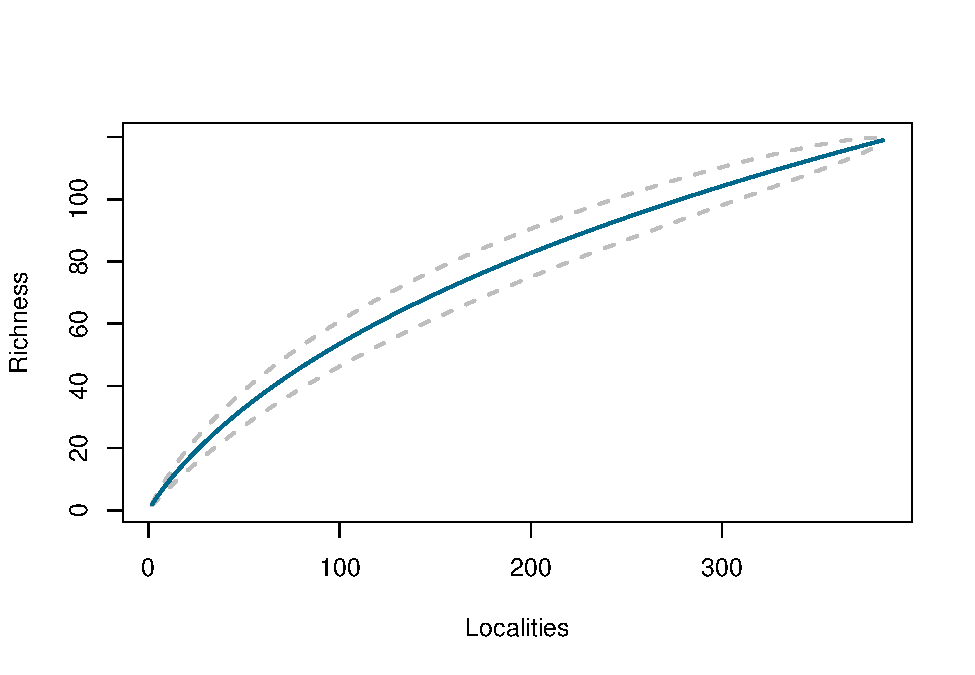
\includegraphics{MA_JJ_files/figure-latex/SACSpecies-1.pdf}
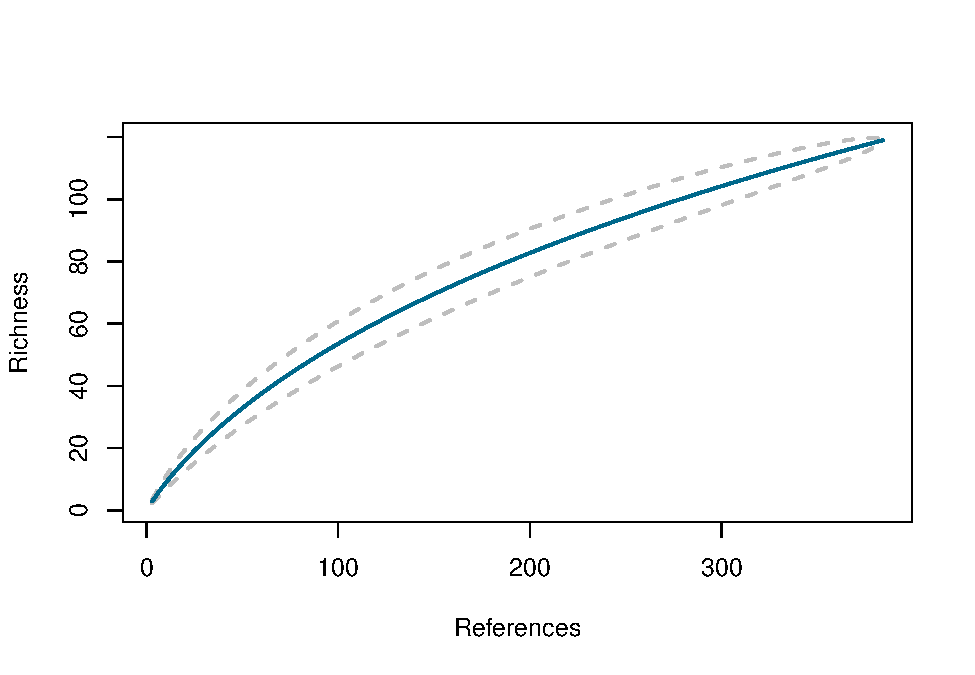
\includegraphics{MA_JJ_files/figure-latex/SACSpecies-2.pdf}

\begin{figure}[htbp]
\centering
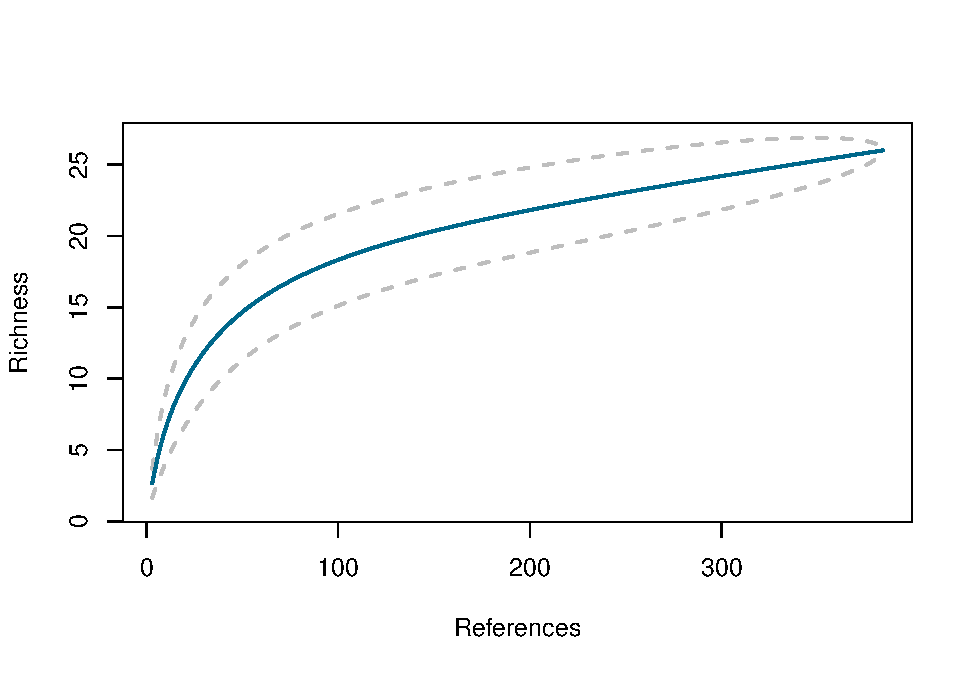
\includegraphics{MA_JJ_files/figure-latex/SACGenera-1.pdf}
\caption{Sampling Accumulation Curve of fossil genera per reference}
\end{figure}

\begin{figure}[htbp]
\centering
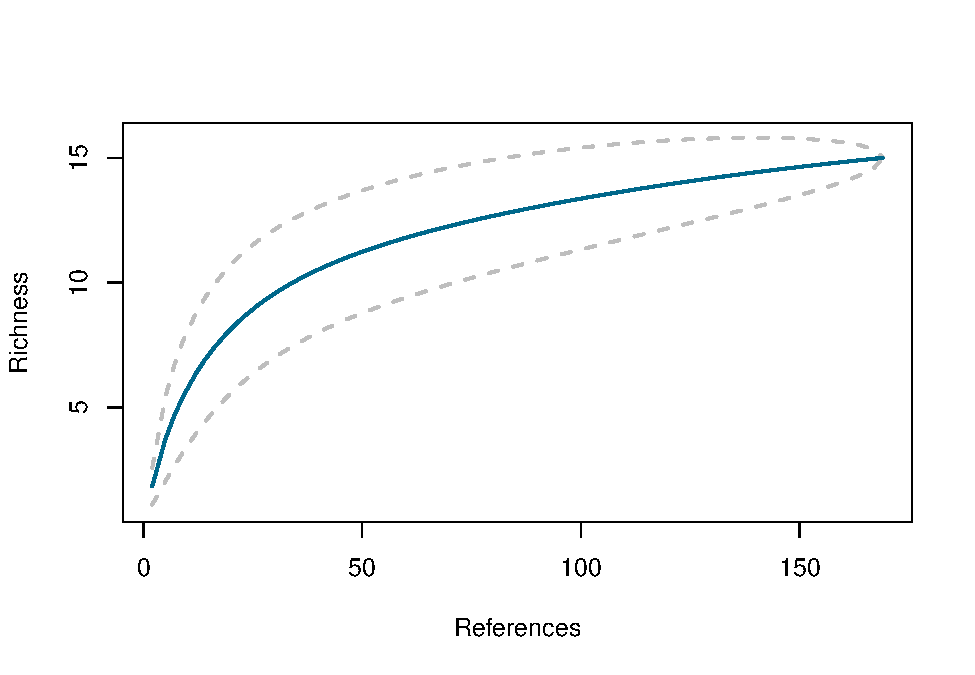
\includegraphics{MA_JJ_files/figure-latex/SACGEurasia-1.pdf}
\caption{Sampling Accumulation Curve of fossil genera per reference,
Eurasia}
\end{figure}

\begin{figure}[htbp]
\centering
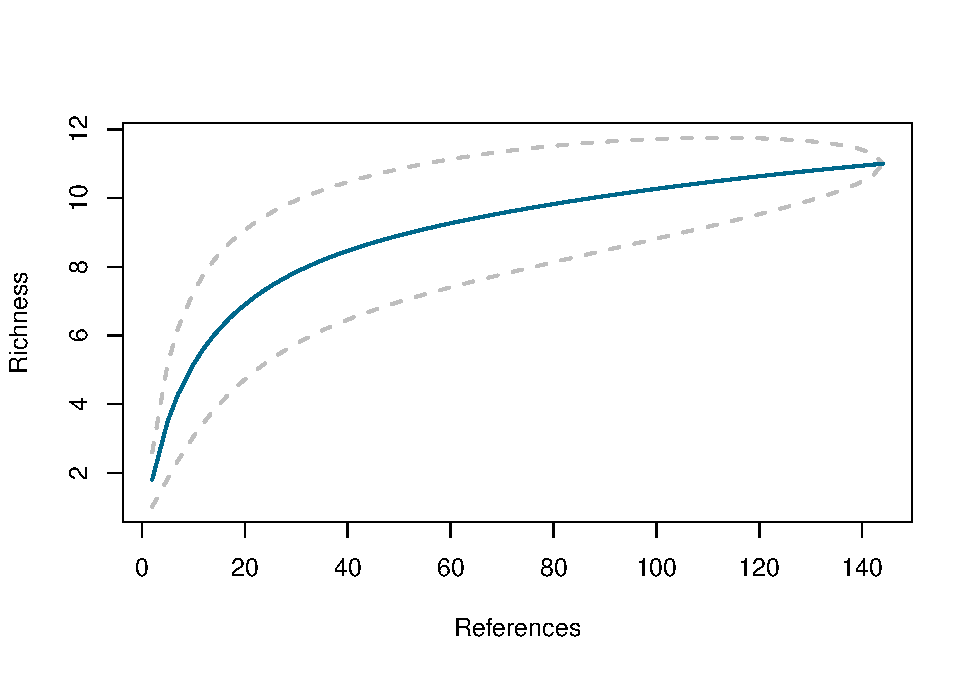
\includegraphics{MA_JJ_files/figure-latex/SACGEurope-1.pdf}
\caption{Sampling Accumulation Curve of fossil genera per reference,
Europe}
\end{figure}

\begin{figure}[htbp]
\centering
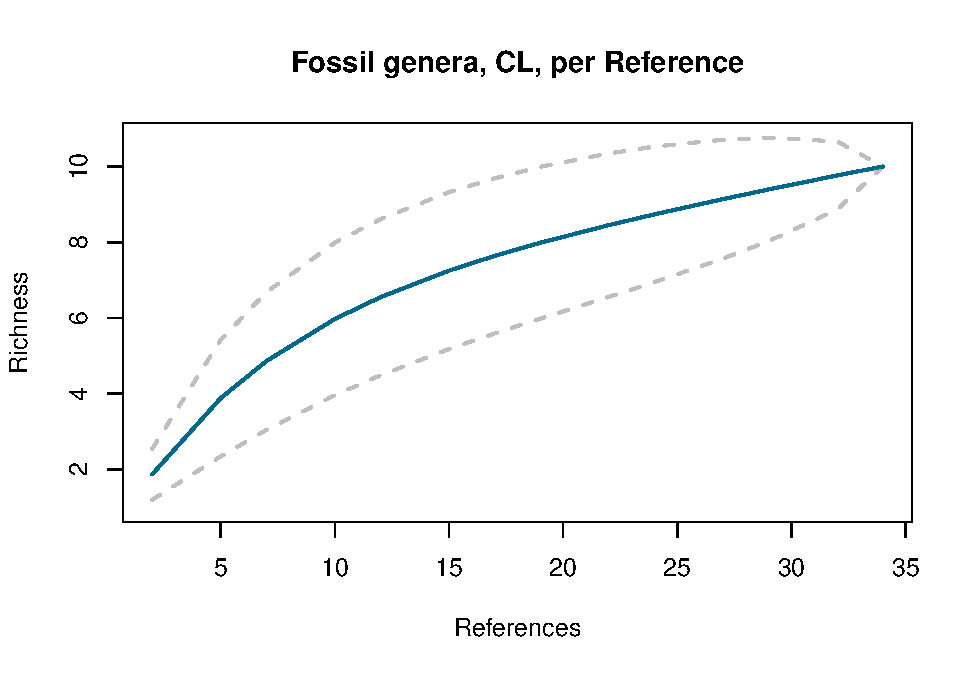
\includegraphics{MA_JJ_files/figure-latex/SACGAfrica-1.pdf}
\caption{Sampling Accumulation Curve of fossil genera per reference,
Africa}
\end{figure}

\begin{figure}[htbp]
\centering
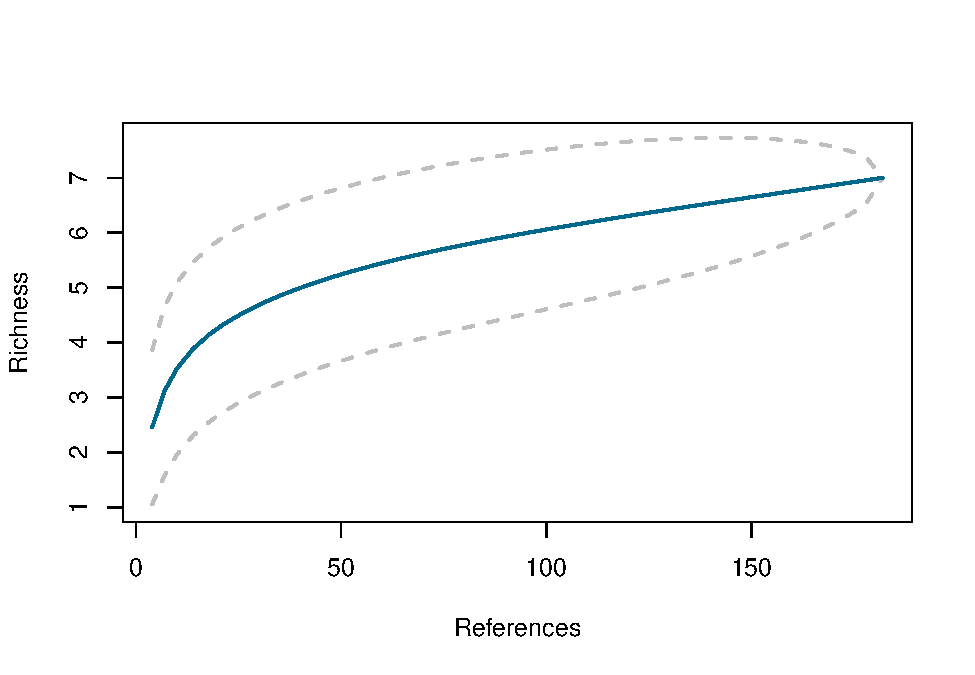
\includegraphics{MA_JJ_files/figure-latex/SACGAmerica-1.pdf}
\caption{Sampling Accumulation Curve of fossil genera per reference,
America}
\end{figure}

\begin{figure}[htbp]
\centering
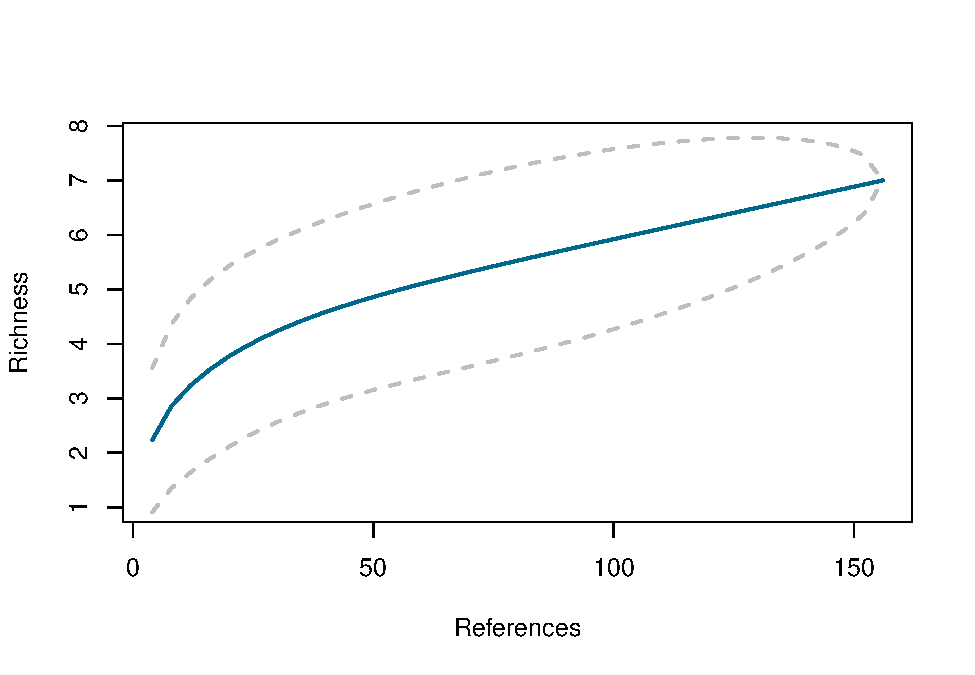
\includegraphics{MA_JJ_files/figure-latex/SACGNAmerica-1.pdf}
\caption{Sampling Accumulation Curve of fossil genera per reference,
N-America}
\end{figure}

\begin{figure}[htbp]
\centering
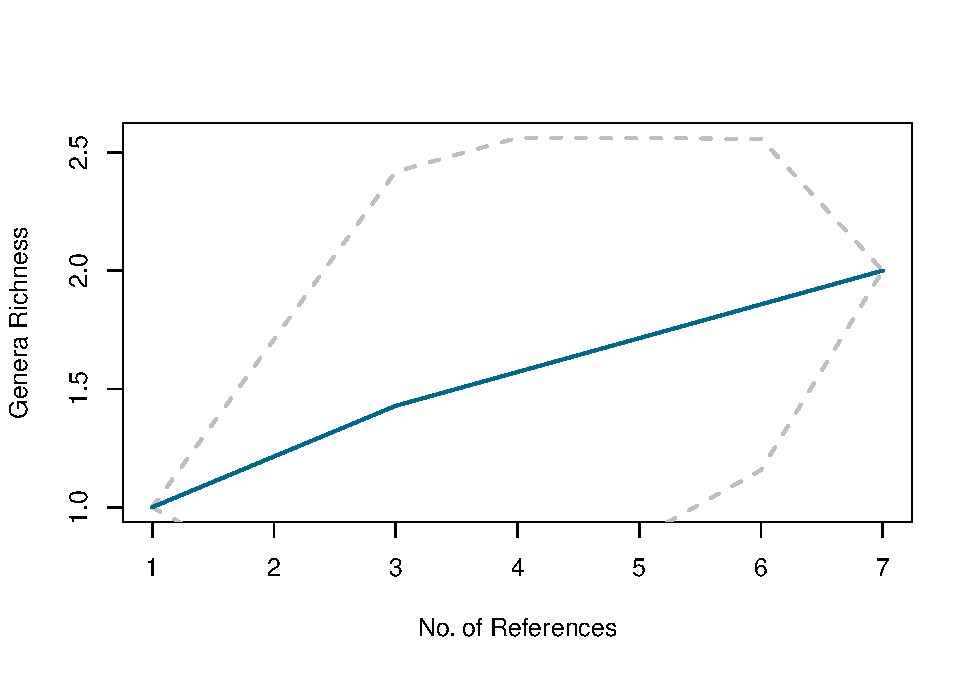
\includegraphics{MA_JJ_files/figure-latex/SACGSAmerica-1.pdf}
\caption{Sampling Accumulation Curve of fossil genera per reference,
S-America}
\end{figure}

\begin{figure}[htbp]
\centering
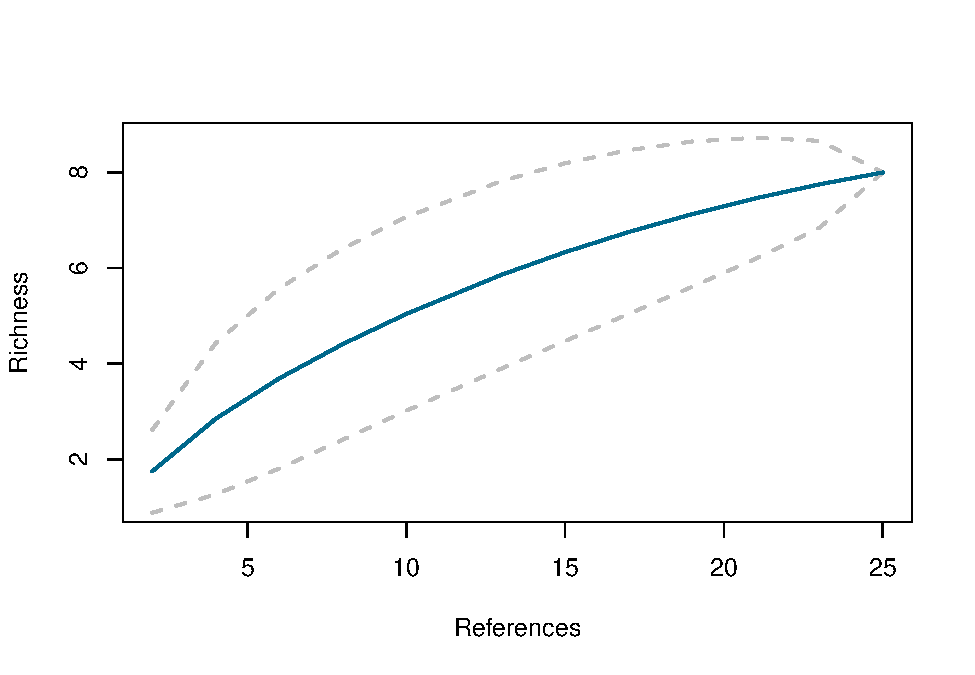
\includegraphics{MA_JJ_files/figure-latex/SACGAsia-1.pdf}
\caption{Sampling Accumulation Curve of fossil genera per reference,
Asia}
\end{figure}

\newpage

\section{Histograms}\label{histograms}

\subsection{all}\label{all}

\begin{verbatim}
## `stat_bin()` using `bins = 30`. Pick better value with `binwidth`.
\end{verbatim}

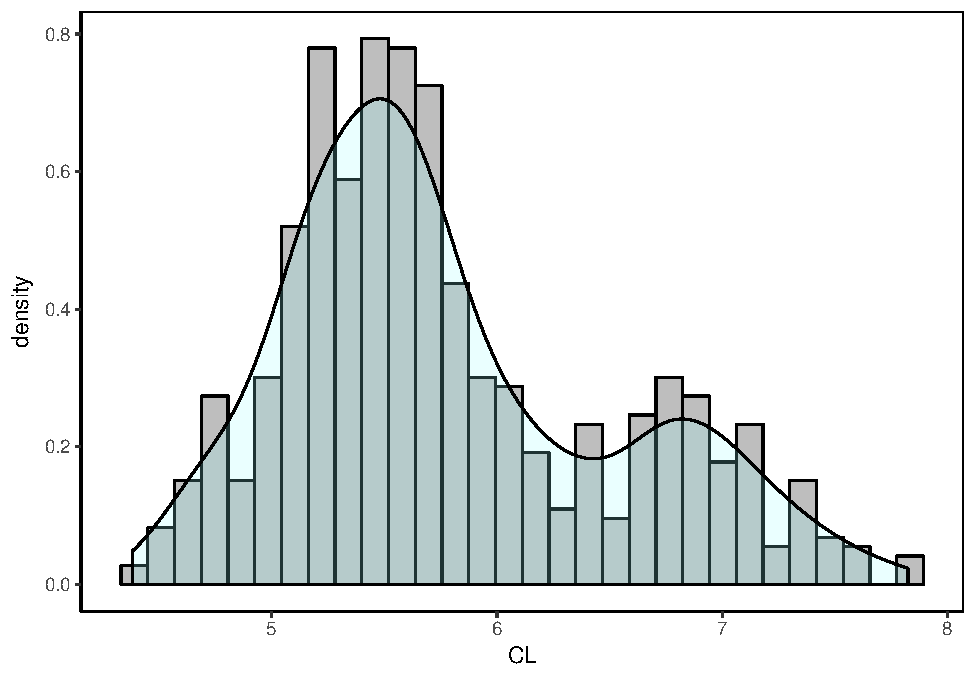
\includegraphics{MA_JJ_files/figure-latex/HistAll-1.pdf}
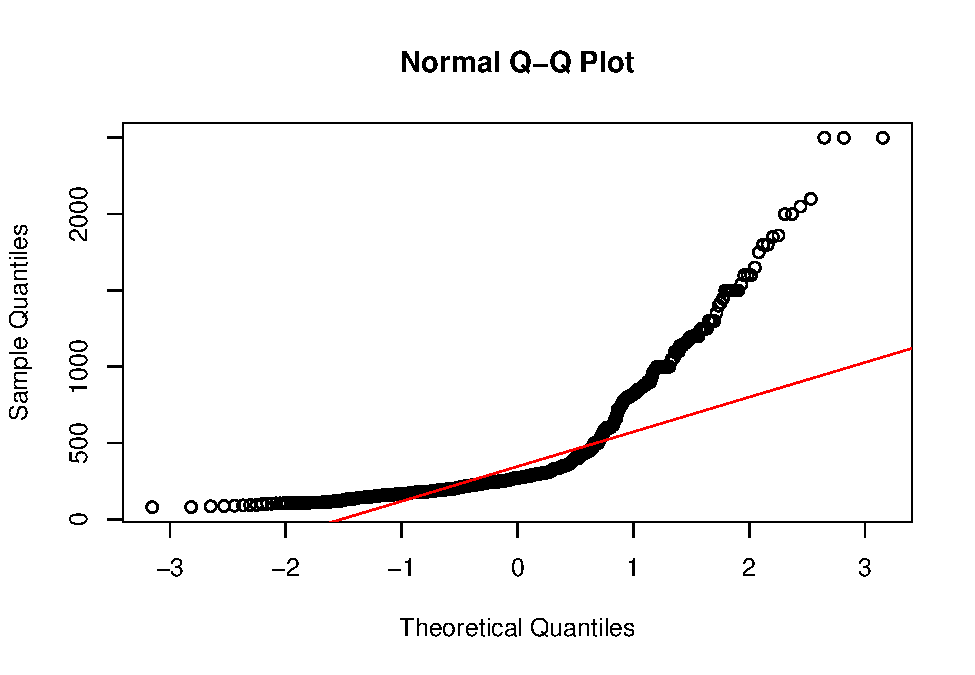
\includegraphics{MA_JJ_files/figure-latex/normalDistribution-1.pdf}
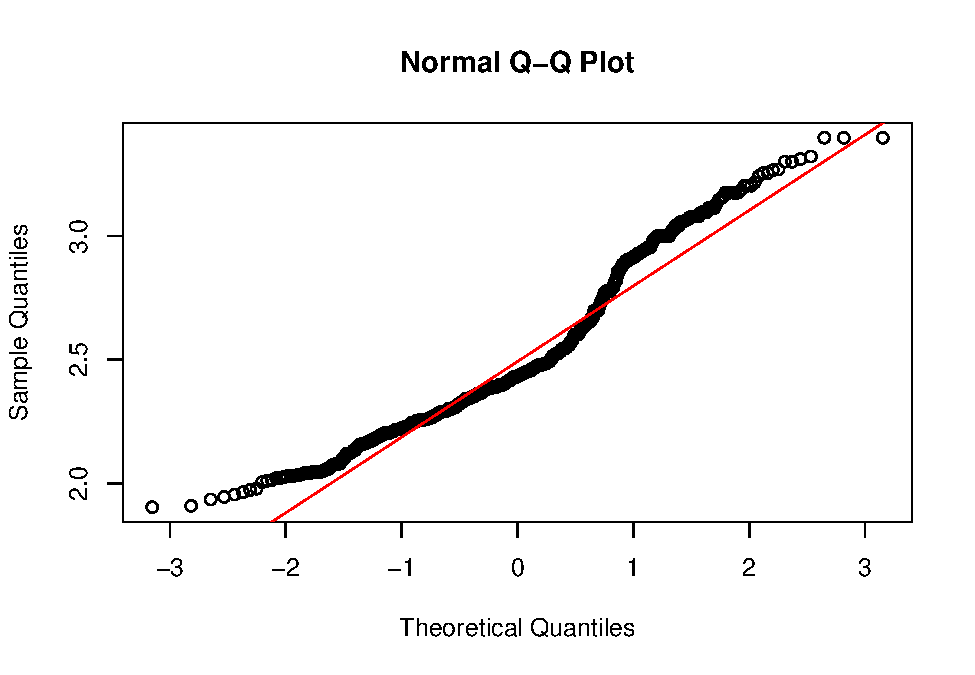
\includegraphics{MA_JJ_files/figure-latex/normalDistribution-2.pdf}

\newpage

\subsection{per time bin}\label{per-time-bin}

\begin{verbatim}
## `stat_bin()` using `bins = 30`. Pick better value with `binwidth`.
\end{verbatim}

\begin{figure}[htbp]
\centering
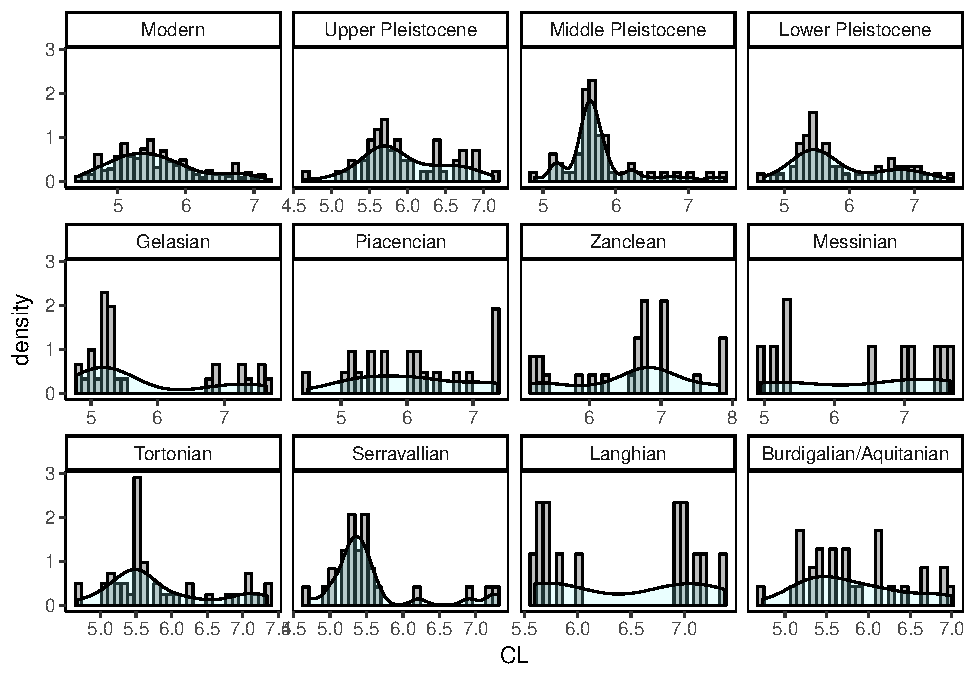
\includegraphics{MA_JJ_files/figure-latex/HistBins-1.pdf}
\caption{Distribution of body size data per time bin, logtransformed.}
\end{figure}

\newpage

\subsection{modern vs.~fossil}\label{modern-vs.fossil}

\begin{verbatim}
## `stat_bin()` using `bins = 30`. Pick better value with `binwidth`.
\end{verbatim}

\begin{figure}[htbp]
\centering
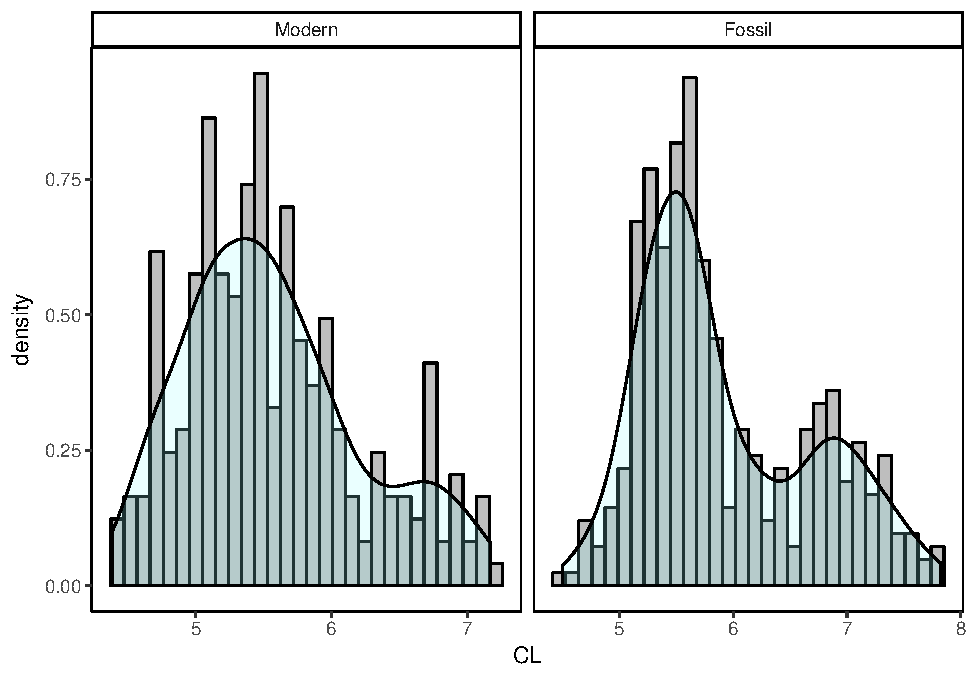
\includegraphics{MA_JJ_files/figure-latex/HistFosMo-1.pdf}
\caption{Distribution of body size data modern vs.~fossil,
logtransformed.}
\end{figure}

\newpage

\subsection{modern vs.~fossil, continental
vs.~insular}\label{modern-vs.fossil-continental-vs.insular}

\begin{verbatim}
## `stat_bin()` using `bins = 30`. Pick better value with `binwidth`.
\end{verbatim}

\begin{figure}[htbp]
\centering
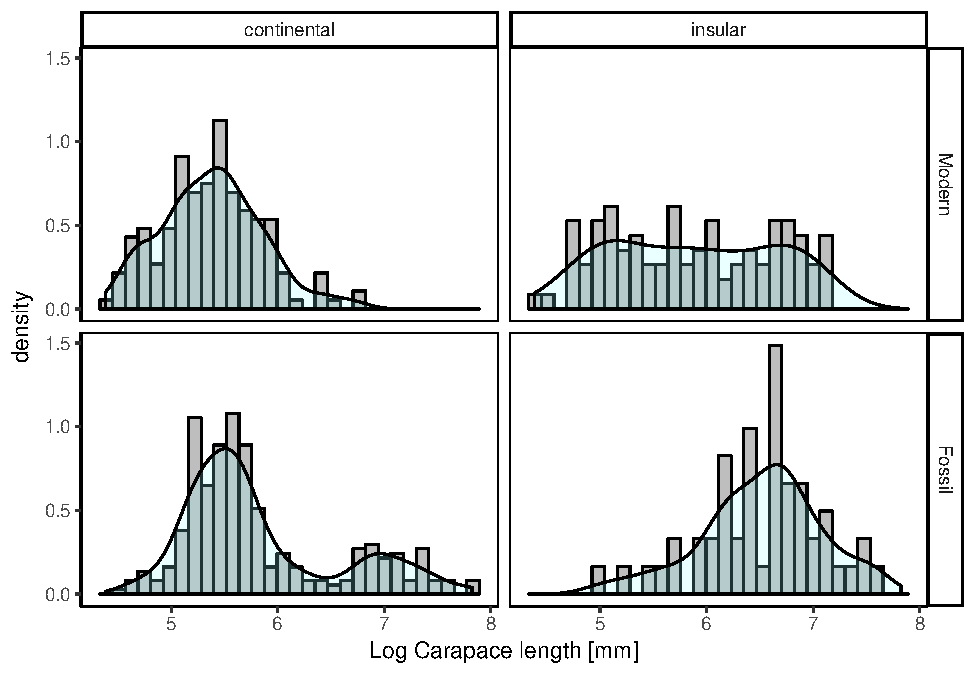
\includegraphics{MA_JJ_files/figure-latex/HistFMCI-1.pdf}
\caption{Distribution of body size data modern vs.~fossil, continental
vs.~insular logtransformed.}
\end{figure}

\newpage

\subsection{continental vs.~insular}\label{continental-vs.insular}

\begin{verbatim}
## `stat_bin()` using `bins = 30`. Pick better value with `binwidth`.
\end{verbatim}

\begin{figure}[htbp]
\centering
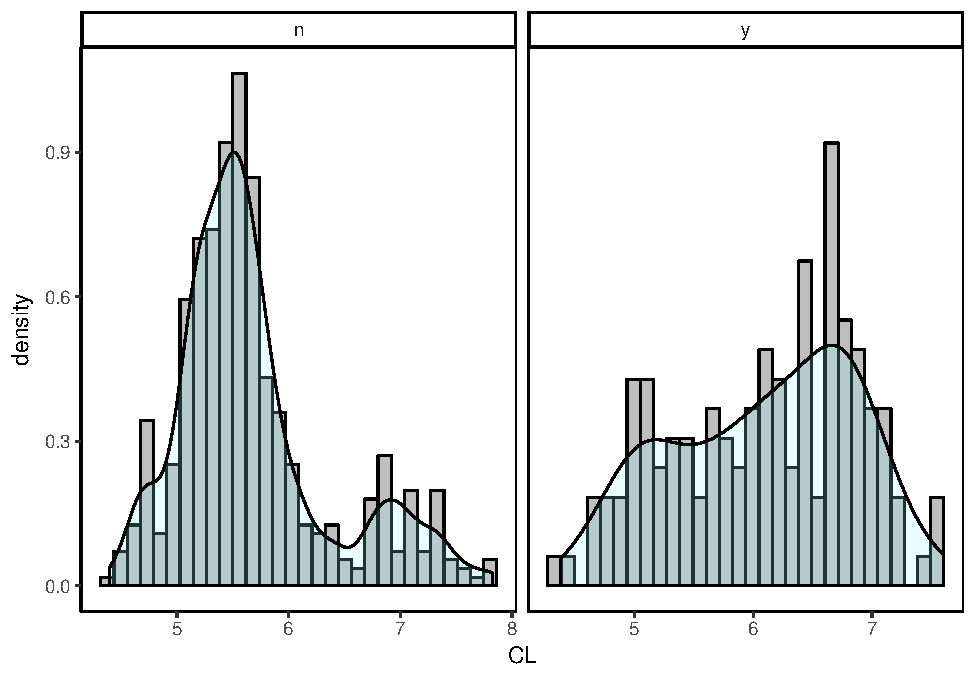
\includegraphics{MA_JJ_files/figure-latex/HistCI-1.pdf}
\caption{Distribution of body site data of continental (n) and
insular(y) species, logtransformed.}
\end{figure}

\newpage

\subsection{continents}\label{continents}

\begin{verbatim}
## `stat_bin()` using `bins = 30`. Pick better value with `binwidth`.
\end{verbatim}

\begin{figure}[htbp]
\centering
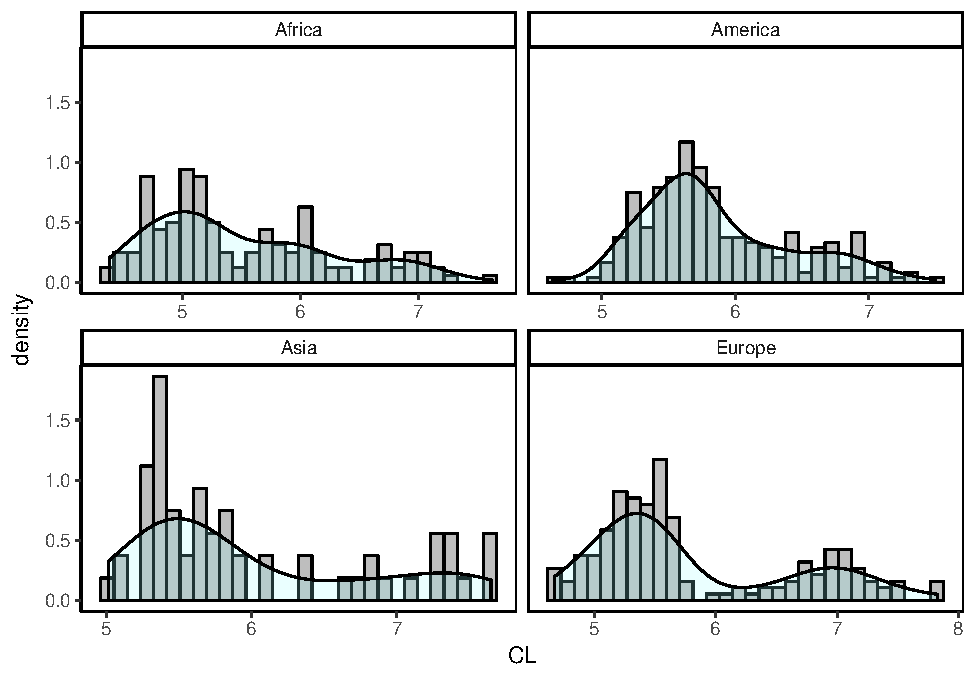
\includegraphics{MA_JJ_files/figure-latex/HistCon-1.pdf}
\caption{Distribution of body site data per continent, logtransformed.}
\end{figure}

\newpage

\subsection{General statistics}\label{general-statistics}

\begin{longtable}[]{@{}rrrrrrrrrrrrl@{}}
\caption{General statistics of body size data: all, per time bin,
insular and continental, per continent (all referring to CL: min, max,
variance, mean, logmean, median, logmedian, skewness, logskewness,
kurosis, logkurtosis}\tabularnewline
\toprule
nCL & min & max & var & mean & logm & med & logmed & skew & logsk & kurt
& logku & Variable\tabularnewline
\midrule
\endfirsthead
\toprule
nCL & min & max & var & mean & logm & med & logmed & skew & logsk & kurt
& logku & Variable\tabularnewline
\midrule
\endhead
616 & 80.00 & 2500 & 164537.80 & 437.2 & 2.5 & 270.5 & 2.4 & 2.14 & 0.69
& 8.00 & 2.73 & all\tabularnewline
253 & 80.00 & 1300 & 67485.50 & 330.3 & 2.4 & 242.0 & 2.4 & 1.83 & 0.58
& 5.87 & 2.69 & Modern\tabularnewline
49 & 102.44 & 1250 & 69690.66 & 445.9 & 2.6 & 334.7 & 2.5 & 1.20 & 0.24
& 3.61 & 2.56 & Upper Pleistocene\tabularnewline
53 & 132.00 & 1800 & 97910.83 & 387.1 & 2.5 & 292.9 & 2.5 & 3.03 & 1.52
& 12.24 & 5.55 & Middle Pleistocene\tabularnewline
57 & 107.80 & 2000 & 161948.82 & 463.5 & 2.5 & 263.0 & 2.4 & 1.74 & 0.73
& 5.76 & 2.40 & Lower Pleistocene\tabularnewline
31 & 118.90 & 2050 & 411224.51 & 555.2 & 2.5 & 194.9 & 2.3 & 1.31 & 0.93
& 3.12 & 2.11 & Gelasian\tabularnewline
21 & 90.00 & 1600 & 270535.82 & 610.6 & 2.6 & 428.0 & 2.6 & 1.00 & 0.14
& 2.50 & 1.99 & Piacencian\tabularnewline
26 & 176.00 & 2500 & 476162.71 & 955.2 & 2.9 & 857.5 & 2.9 & 1.11 &
-0.40 & 3.56 & 2.30 & Zanclean\tabularnewline
10 & 140.00 & 2100 & 602611.21 & 948.9 & 2.8 & 916.0 & 2.9 & 0.26 &
-0.22 & 1.49 & 1.29 & Messinian\tabularnewline
45 & 107.00 & 1540 & 175470.12 & 462.7 & 2.5 & 250.0 & 2.4 & 1.49 & 0.81
& 3.74 & 2.54 & Tortonian\tabularnewline
27 & 111.00 & 1500 & 126060.40 & 337.7 & 2.4 & 220.0 & 2.3 & 2.49 & 1.77
& 7.77 & 5.30 & Serravallian\tabularnewline
14 & 270.00 & 1600 & 230451.33 & 747.9 & 2.8 & 700.0 & 2.8 & 0.30 & 0.03
& 1.55 & 1.18 & Langhian\tabularnewline
30 & 113.00 & 1100 & 76288.76 & 406.8 & 2.5 & 302.4 & 2.5 & 1.27 & 0.45
& 3.45 & 2.26 & Burdigalian/Aquitanian\tabularnewline
253 & 80.00 & 1300 & 67485.50 & 330.3 & 2.4 & 242.0 & 2.4 & 1.83 & 0.58
& 5.87 & 2.69 & Modern\tabularnewline
363 & 90.00 & 2500 & 219004.66 & 511.7 & 2.6 & 285.6 & 2.5 & 1.83 & 0.68
& 6.11 & 2.42 & Fossil\tabularnewline
469 & 81.00 & 2500 & 157808.79 & 392.9 & 2.5 & 250.0 & 2.4 & 2.65 & 1.07
& 10.57 & 3.74 & continental\tabularnewline
147 & 80.00 & 2000 & 160834.35 & 578.5 & 2.6 & 500.0 & 2.7 & 1.02 &
-0.27 & 3.95 & 2.05 & insular\tabularnewline
157 & 81.00 & 830 & 17009.02 & 244.0 & 2.3 & 221.0 & 2.3 & 1.92 & 0.29 &
8.09 & 2.98 & modern-con\tabularnewline
96 & 80.00 & 1300 & 118641.09 & 471.5 & 2.6 & 353.0 & 2.5 & 0.82 & 0.01
& 2.47 & 1.77 & modern-ins\tabularnewline
312 & 90.00 & 2500 & 212116.79 & 467.9 & 2.5 & 270.0 & 2.4 & 2.11 & 0.96
& 7.25 & 2.96 & fossil-con\tabularnewline
51 & 150.00 & 2000 & 180825.40 & 780.0 & 2.8 & 750.0 & 2.9 & 1.11 &
-0.40 & 4.02 & 3.18 & fossil-ins\tabularnewline
142 & 80.00 & 2050 & 112417.26 & 347.7 & 2.4 & 193.5 & 2.3 & 2.10 & 0.68
& 7.97 & 2.48 & Africa\tabularnewline
242 & 102.44 & 1800 & 82209.71 & 415.0 & 2.5 & 302.2 & 2.5 & 1.92 & 0.75
& 6.79 & 2.91 & America\tabularnewline
59 & 150.00 & 2100 & 323123.20 & 585.5 & 2.6 & 280.0 & 2.4 & 1.43 & 0.85
& 3.61 & 2.24 & Asia\tabularnewline
173 & 107.00 & 2500 & 254222.84 & 491.2 & 2.5 & 245.0 & 2.4 & 1.86 &
0.81 & 6.30 & 2.34 & Europe\tabularnewline
\bottomrule
\end{longtable}

\newpage

\section{Boxplots}\label{boxplots}

\subsection{genera per time bins}\label{genera-per-time-bins}

\begin{figure}[htbp]
\centering
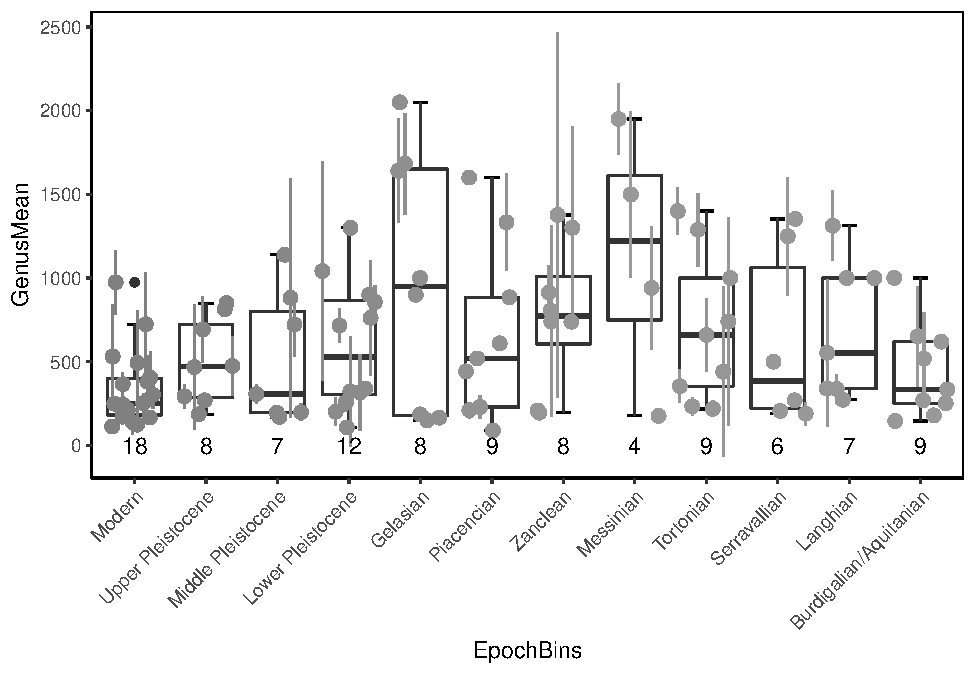
\includegraphics{MA_JJ_files/figure-latex/BPGBins-1.pdf}
\caption{Boxplots of mean CL per time bin, including mean and sd CL for
each genus (as pointrange).}
\end{figure}

\newpage

\subsection{continental vs.~insular per time
bin}\label{continental-vs.insular-per-time-bin}

\begin{figure}[htbp]
\centering
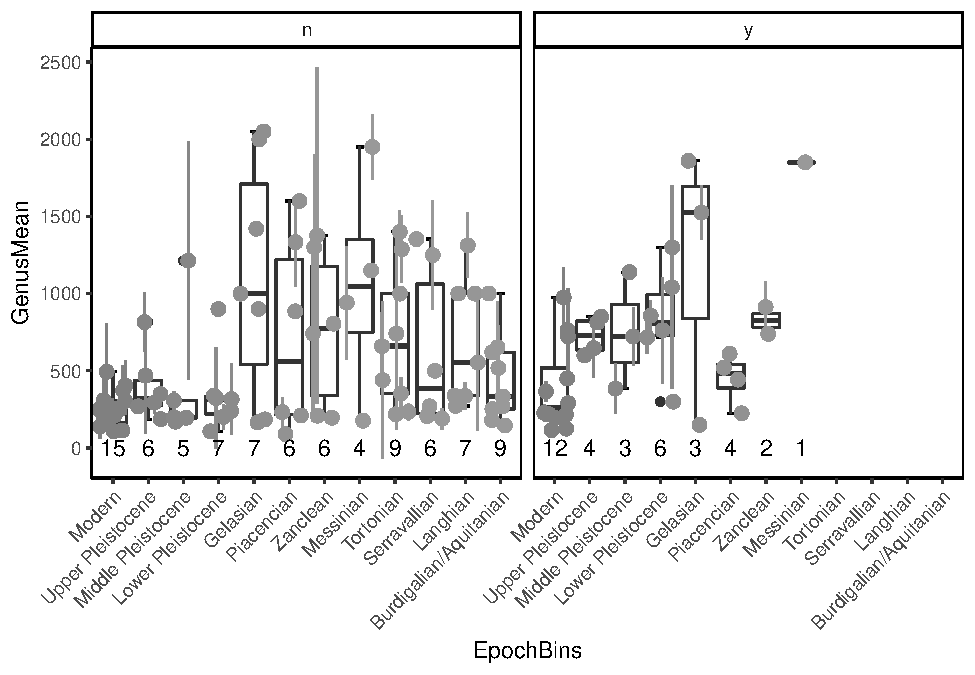
\includegraphics{MA_JJ_files/figure-latex/BPGBinsCI-1.pdf}
\caption{Boxplots of each genus per time bin, continental vs.~insular
species.}
\end{figure}

\newpage

\subsection{fossil vs.~modern}\label{fossil-vs.modern}

\begin{figure}[htbp]
\centering
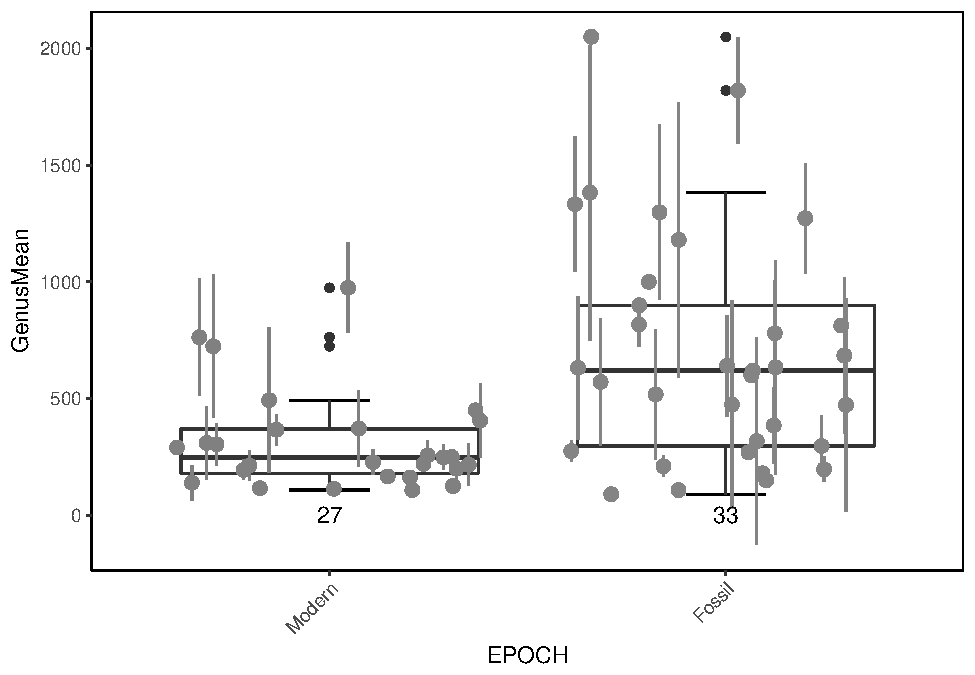
\includegraphics{MA_JJ_files/figure-latex/BPMF-1.pdf}
\caption{Boxplots fossil vs.~modern.}
\end{figure}

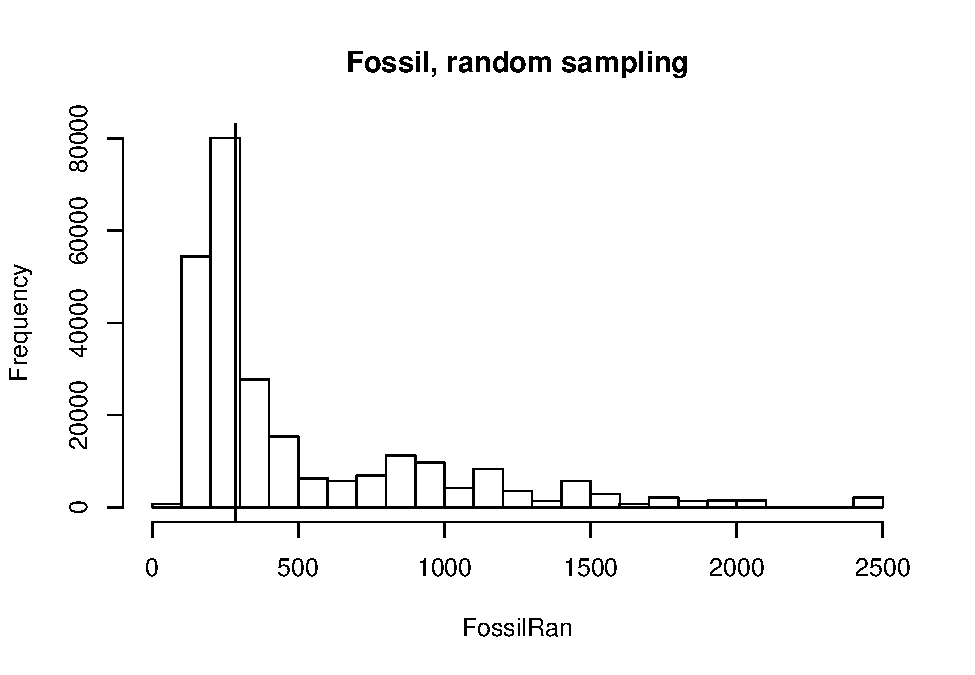
\includegraphics{MA_JJ_files/figure-latex/RSFM-1.pdf}

\begin{verbatim}
## [1] 330.3495
\end{verbatim}

\begin{verbatim}
## [1] 486.6345
\end{verbatim}

\begin{verbatim}
## 
##  Wilcoxon rank sum test with continuity correction
## 
## data:  Modern and Fossil
## W = 23743, p-value = 4.824e-07
## alternative hypothesis: true location shift is less than 0
\end{verbatim}

Wilcoxon Rank Sum Test (unpaired data):

modern \textless{} fossil (P = \(4.8236434\times 10^{-7}\))

\newpage

\subsection{fossil vs.~modern, continental
vs.~insular}\label{fossil-vs.modern-continental-vs.insular}

\begin{figure}[htbp]
\centering
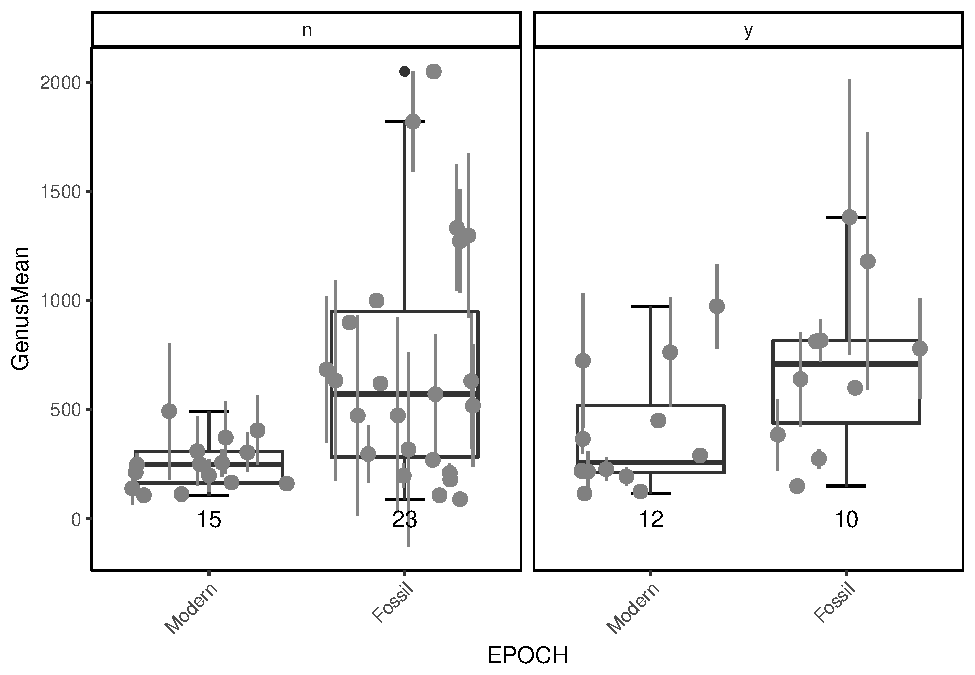
\includegraphics{MA_JJ_files/figure-latex/BPFMCI-1.pdf}
\caption{Boxplots fossil vs.~modern, continental vs.~insular species.}
\end{figure}

\begin{verbatim}
## [1] 51
\end{verbatim}

\begin{verbatim}
## [1] 51
\end{verbatim}

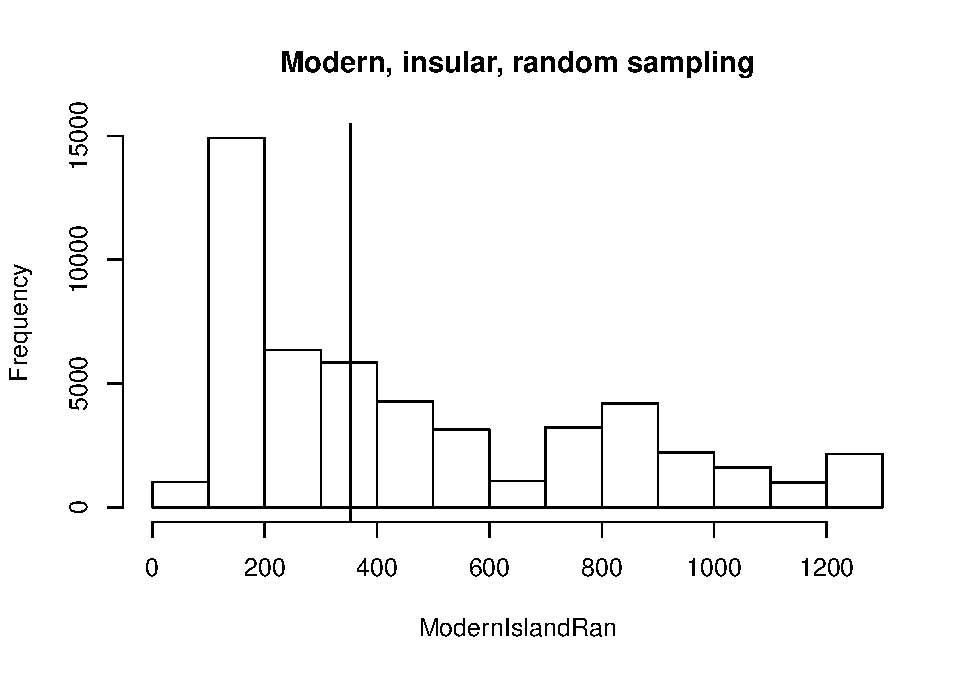
\includegraphics{MA_JJ_files/figure-latex/RSMFCI-1.pdf}

\begin{verbatim}
## 
##  Wilcoxon rank sum test with continuity correction
## 
## data:  ModernIsland and FossilIsland
## W = 656.5, p-value = 8.268e-06
## alternative hypothesis: true location shift is less than 0
\end{verbatim}

\begin{verbatim}
## [1] 157
\end{verbatim}

\begin{verbatim}
## [1] 157
\end{verbatim}

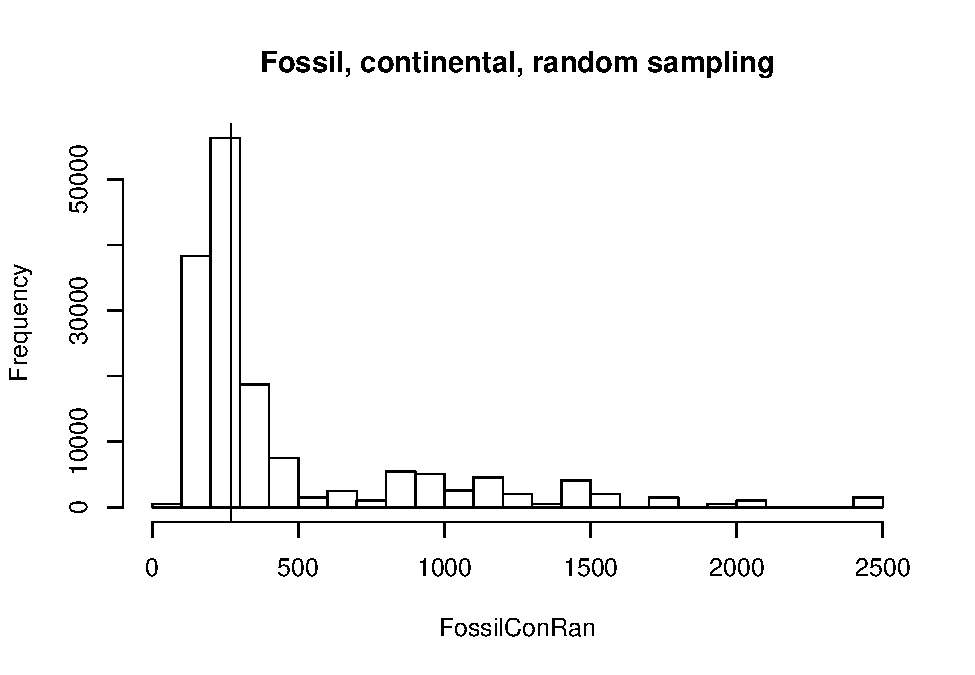
\includegraphics{MA_JJ_files/figure-latex/RSMFCI-2.pdf}

\begin{verbatim}
## 
##  Wilcoxon rank sum test with continuity correction
## 
## data:  ModernCon and FossilCon
## W = 8352.5, p-value = 3.958e-07
## alternative hypothesis: true location shift is less than 0
\end{verbatim}

Wilcoxon Rank Sum Test (unpaired data):

modern continental \textless{} fossil continental (P =
\(3.9578046\times 10^{-7}\))

modern insular \textless{} fossil insular (P =
\(8.2677805\times 10^{-6}\))

\newpage

\subsection{continental vs.~insular}\label{continental-vs.insular-1}

\begin{figure}[htbp]
\centering
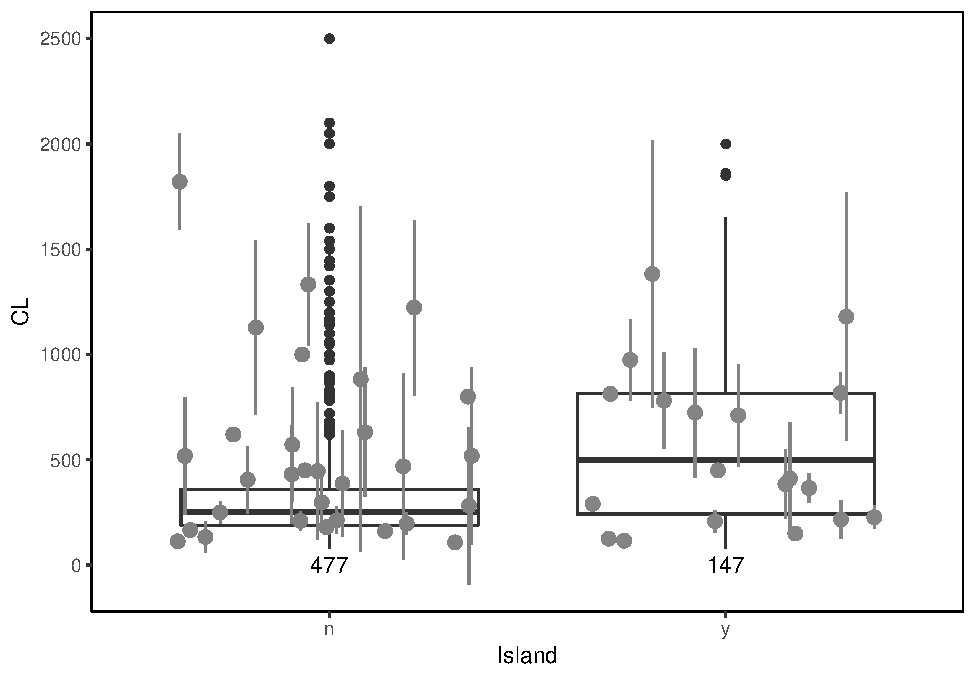
\includegraphics{MA_JJ_files/figure-latex/BPCI-1.pdf}
\caption{Boxplot continental vs.~insular, genera summarised}
\end{figure}

\begin{verbatim}
## [1] 147
\end{verbatim}

\begin{verbatim}
## [1] 147
\end{verbatim}

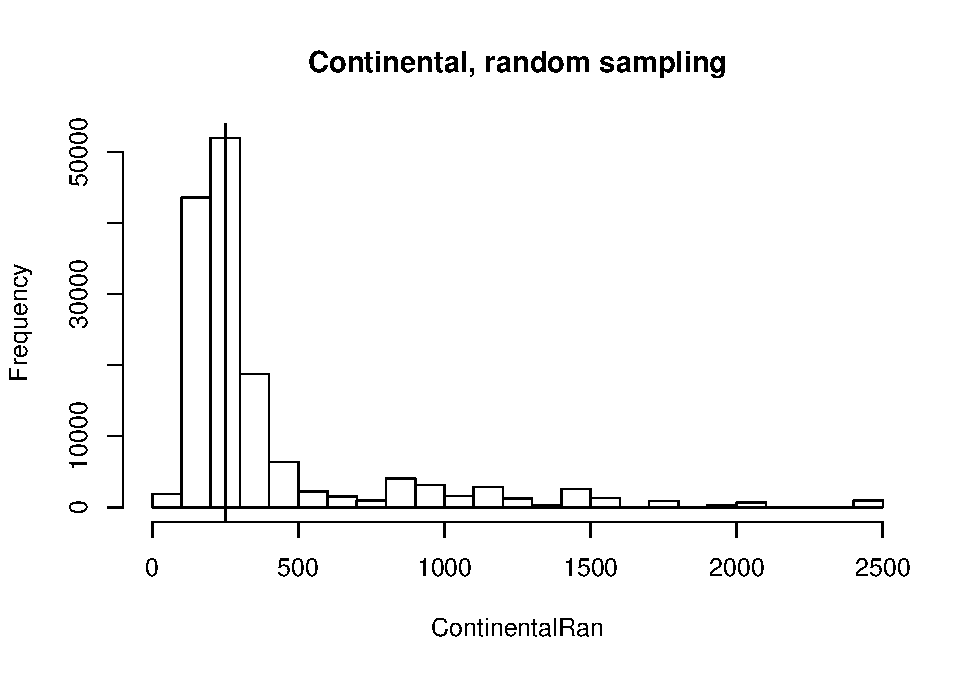
\includegraphics{MA_JJ_files/figure-latex/RSCI-1.pdf}

\begin{verbatim}
## 
##  Wilcoxon rank sum test with continuity correction
## 
## data:  Insular and Continental
## W = 14424, p-value = 3.426e-07
## alternative hypothesis: true location shift is greater than 0
\end{verbatim}

Wilcoxon Rank Sum Test (unpaired data):

continental \textless{} insular (P = \(3.4257949\times 10^{-7}\))

\newpage

\subsection{continental vs.~insular per time
bin}\label{continental-vs.insular-per-time-bin-1}

\begin{figure}[htbp]
\centering
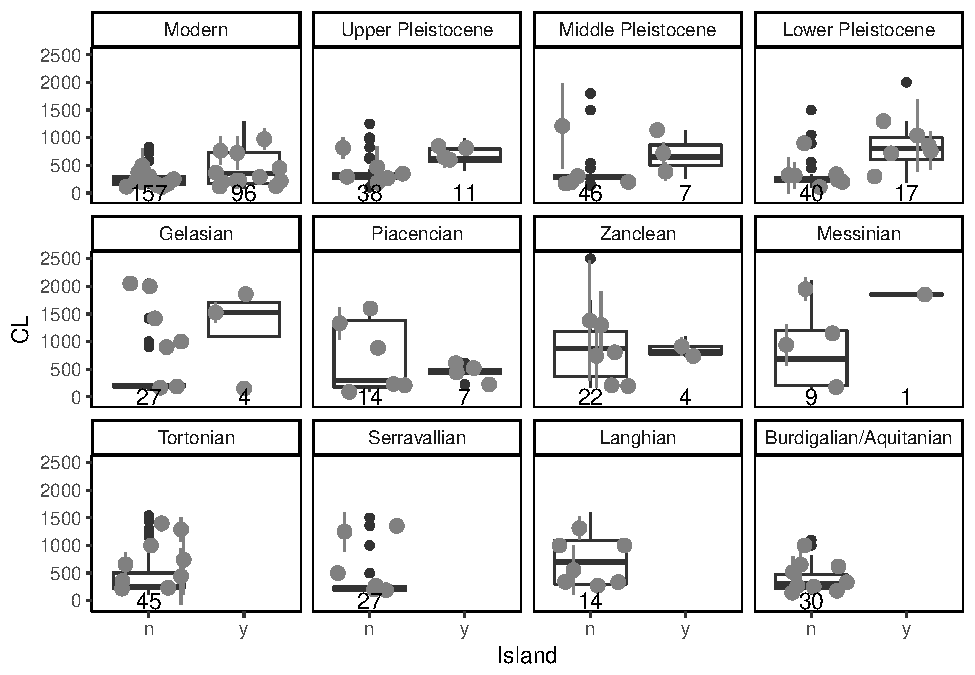
\includegraphics{MA_JJ_files/figure-latex/BPCIBins-1.pdf}
\caption{Boxplot continental vs.~insular, genera summarised}
\end{figure}

\newpage

\subsection{continents}\label{continents-1}

\begin{figure}[htbp]
\centering
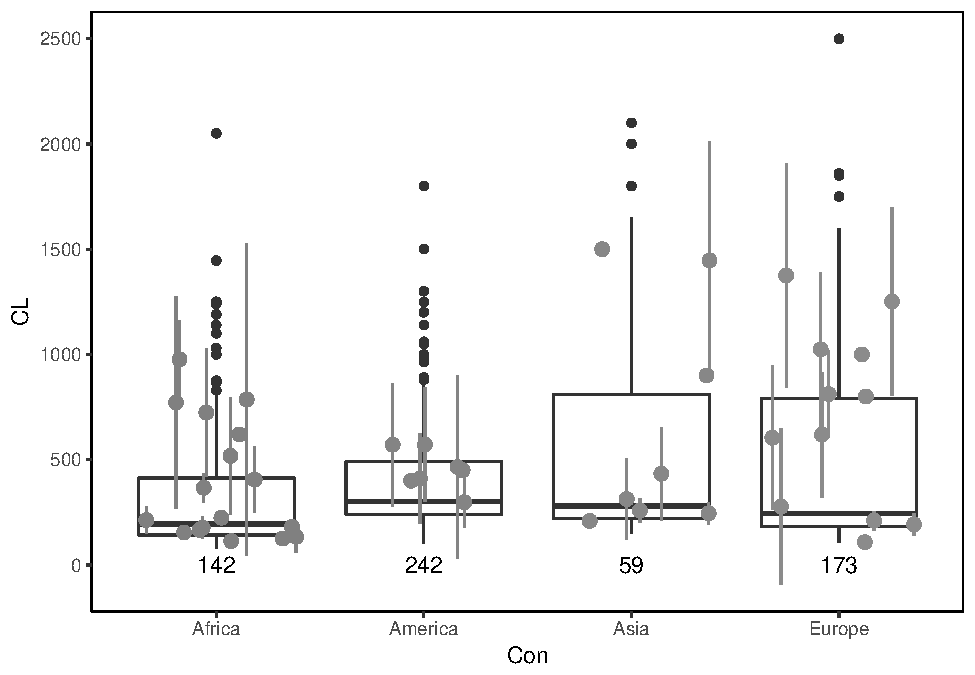
\includegraphics{MA_JJ_files/figure-latex/BPCon-1.pdf}
\caption{Boxplot: body size on different continents, genera summarised}
\end{figure}

\begin{verbatim}
## [1] 142
\end{verbatim}

\begin{verbatim}
## [1] 347.6887
\end{verbatim}

\begin{verbatim}
## [1] 142
\end{verbatim}

\begin{verbatim}
## [1] 428.2396
\end{verbatim}

\begin{verbatim}
## [1] 59
\end{verbatim}

\begin{verbatim}
## [1] 173
\end{verbatim}

\begin{verbatim}
## [1] 142
\end{verbatim}

\begin{verbatim}
## [1] 514.8937
\end{verbatim}

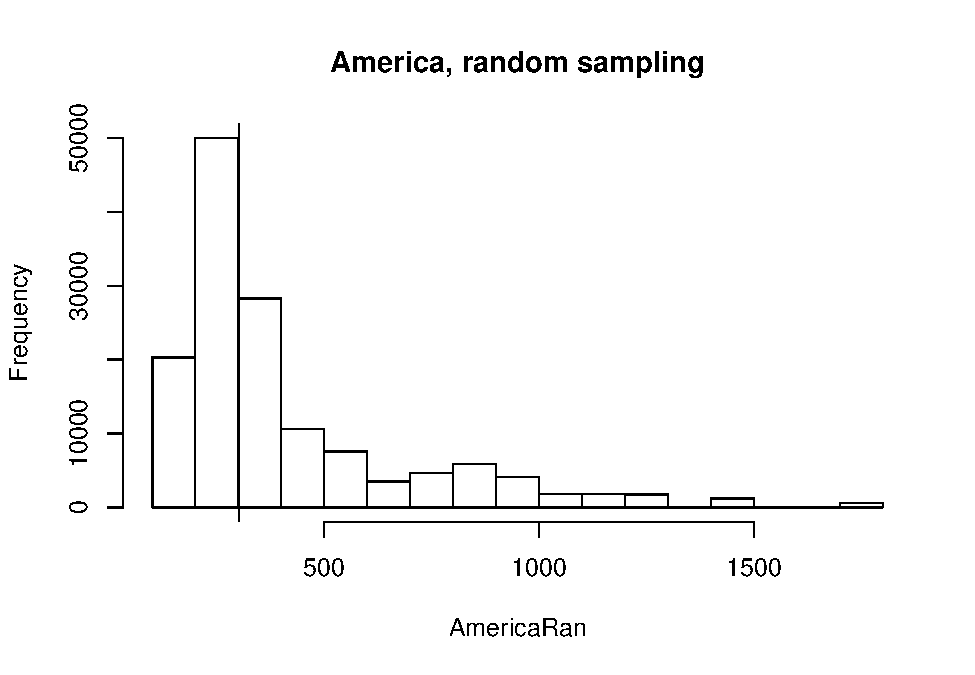
\includegraphics{MA_JJ_files/figure-latex/RSCon-1.pdf}
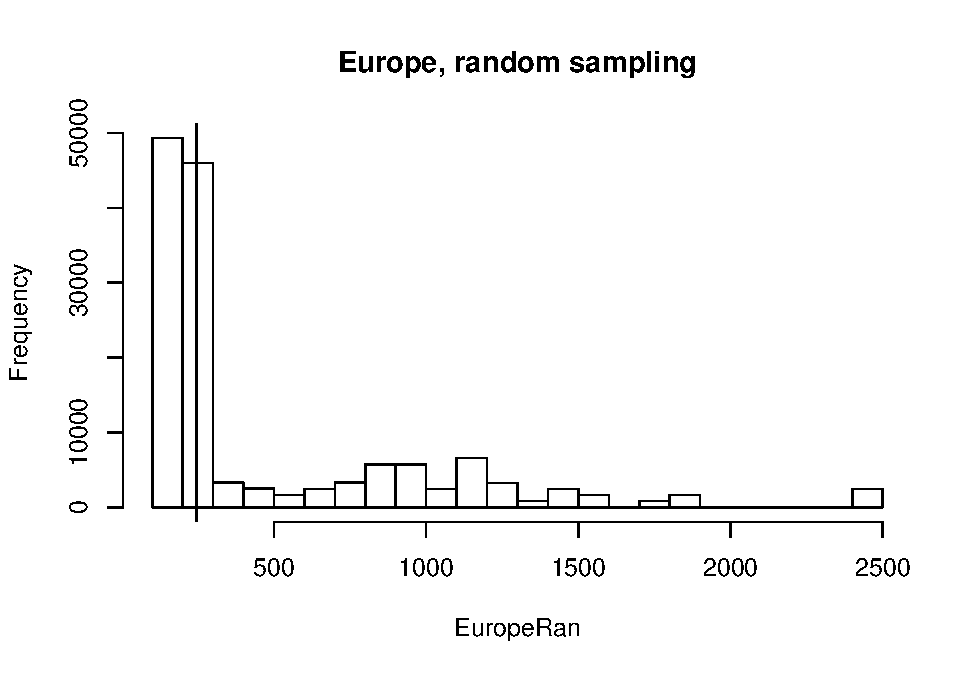
\includegraphics{MA_JJ_files/figure-latex/RSCon-2.pdf}
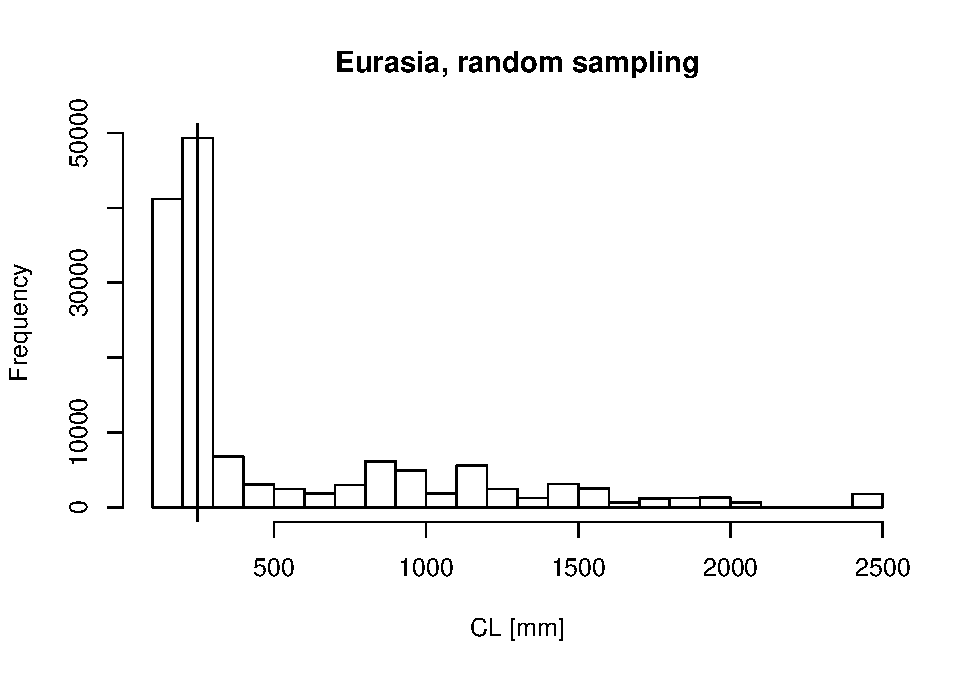
\includegraphics{MA_JJ_files/figure-latex/RSCon-3.pdf}

\begin{verbatim}
## 
##  Kruskal-Wallis rank sum test
## 
## data:  list(Africa, America, Eurasia, Europe)
## Kruskal-Wallis chi-squared = 34.01, df = 3, p-value = 1.972e-07
\end{verbatim}

Kruskal-Wallis-Test:

Continent means differ (P = \(1.9716277\times 10^{-7}\)) (still have to
look into the details\ldots{})

\newpage

\subsection{continents, continental
vs.~insular}\label{continents-continental-vs.insular}

\begin{figure}[htbp]
\centering
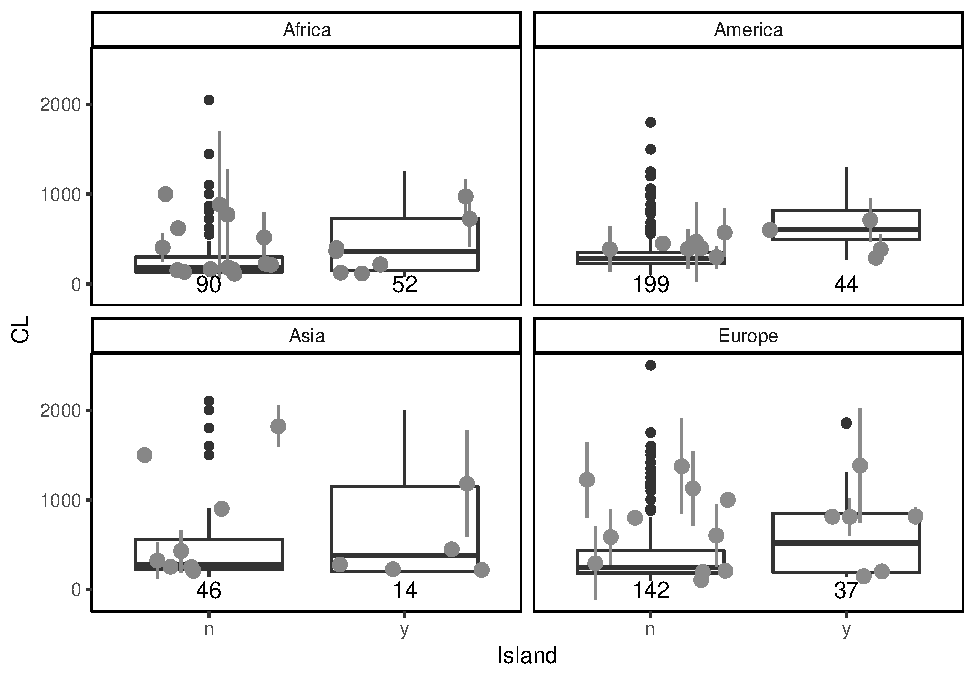
\includegraphics{MA_JJ_files/figure-latex/BPConCI-1.pdf}
\caption{Boxplot: body size on different continents, genera summarised}
\end{figure}

\newpage

\section{paleoTS analysis}\label{paleots-analysis}

\subsection{all (continental and
insular)}\label{all-continental-and-insular}

\subsubsection{genera (all)}\label{genera-all}

\begin{longtable}[]{@{}rrrr@{}}
\caption{paleoTS object, all data}\tabularnewline
\toprule
tt & mm & vv & nn\tabularnewline
\midrule
\endfirsthead
\toprule
tt & mm & vv & nn\tabularnewline
\midrule
\endhead
0.0000005 & 401.9641 & 102306.64 & 4\tabularnewline
0.0058500 & 314.1859 & 42607.58 & 18\tabularnewline
0.0688500 & 506.3265 & 64620.11 & 8\tabularnewline
0.4535000 & 516.4053 & 155241.85 & 7\tabularnewline
1.2935000 & 593.8669 & 147507.20 & 12\tabularnewline
2.1970000 & 971.8850 & 580540.76 & 8\tabularnewline
3.0940000 & 658.0826 & 271043.73 & 9\tabularnewline
4.4660000 & 785.0792 & 187937.61 & 8\tabularnewline
6.2890000 & 1141.9375 & 584378.85 & 4\tabularnewline
9.4270000 & 703.9570 & 195766.19 & 9\tabularnewline
12.7140000 & 628.3020 & 285258.36 & 6\tabularnewline
14.8950000 & 687.9619 & 169914.58 & 7\tabularnewline
19.5000000 & 441.5420 & 78467.65 & 9\tabularnewline
\bottomrule
\end{longtable}

\begin{figure}[htbp]
\centering
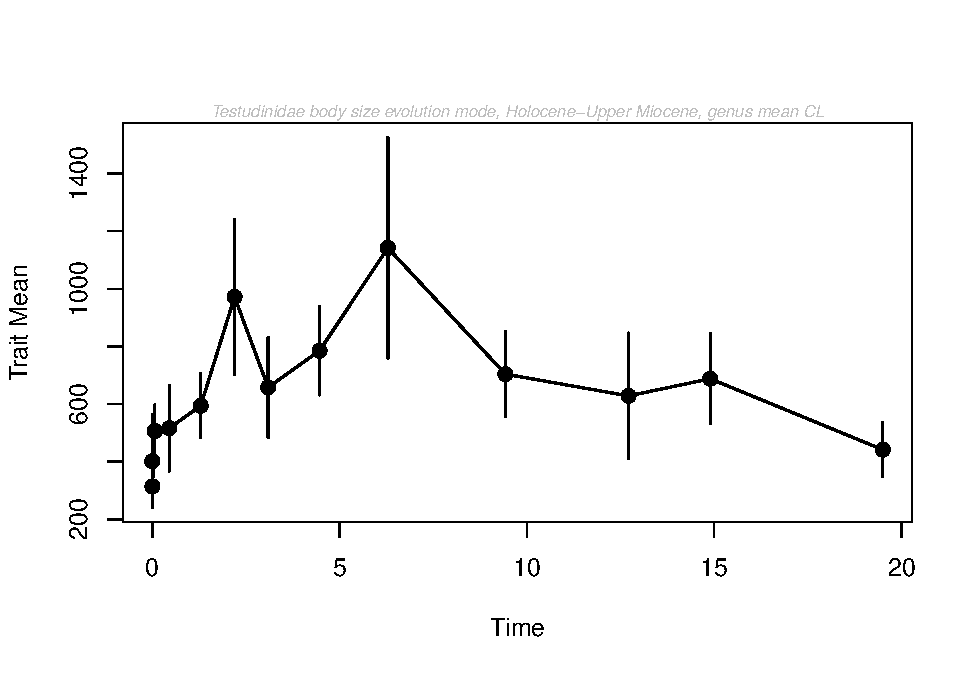
\includegraphics{MA_JJ_files/figure-latex/paleoTSAll-1.pdf}
\caption{paleoTS plot with genus mean, all}
\end{figure}

\begin{longtable}[]{@{}lrrrr@{}}
\caption{Model-fitting results for testudinidae, genera,
all}\tabularnewline
\toprule
& logL & K & AICc & Akaike.wt\tabularnewline
\midrule
\endfirsthead
\toprule
& logL & K & AICc & Akaike.wt\tabularnewline
\midrule
\endhead
GRW & -81.31790 & 2 & 167.9691 & 0.161\tabularnewline
URW & -82.05721 & 1 & 166.5144 & 0.332\tabularnewline
Stasis & -80.16802 & 2 & 165.6694 & 0.507\tabularnewline
\bottomrule
\end{longtable}

\newpage

\subsection{continental (excluding insular
species)}\label{continental-excluding-insular-species}

\subsubsection{genera (continental)}\label{genera-continental}

\begin{longtable}[]{@{}rrrr@{}}
\caption{paleoTS object, continental}\tabularnewline
\toprule
tt & mm & vv & nn\tabularnewline
\midrule
\endfirsthead
\toprule
tt & mm & vv & nn\tabularnewline
\midrule
\endhead
0.0000005 & 233.1680 & 8331.753 & 3\tabularnewline
0.0058500 & 241.7917 & 13004.928 & 15\tabularnewline
0.0688500 & 397.4606 & 50619.392 & 6\tabularnewline
0.4535000 & 416.9341 & 200982.124 & 5\tabularnewline
1.2935000 & 346.8484 & 66240.066 & 7\tabularnewline
2.1970000 & 1103.1067 & 595507.933 & 7\tabularnewline
3.0940000 & 725.4156 & 414253.291 & 6\tabularnewline
4.4660000 & 771.3833 & 259173.082 & 6\tabularnewline
6.2890000 & 1054.4375 & 531455.932 & 4\tabularnewline
9.4270000 & 703.9570 & 195766.185 & 9\tabularnewline
12.7140000 & 628.3020 & 285258.362 & 6\tabularnewline
14.8950000 & 687.9619 & 169914.577 & 7\tabularnewline
19.5000000 & 441.5420 & 78467.646 & 9\tabularnewline
\bottomrule
\end{longtable}

\begin{figure}[htbp]
\centering
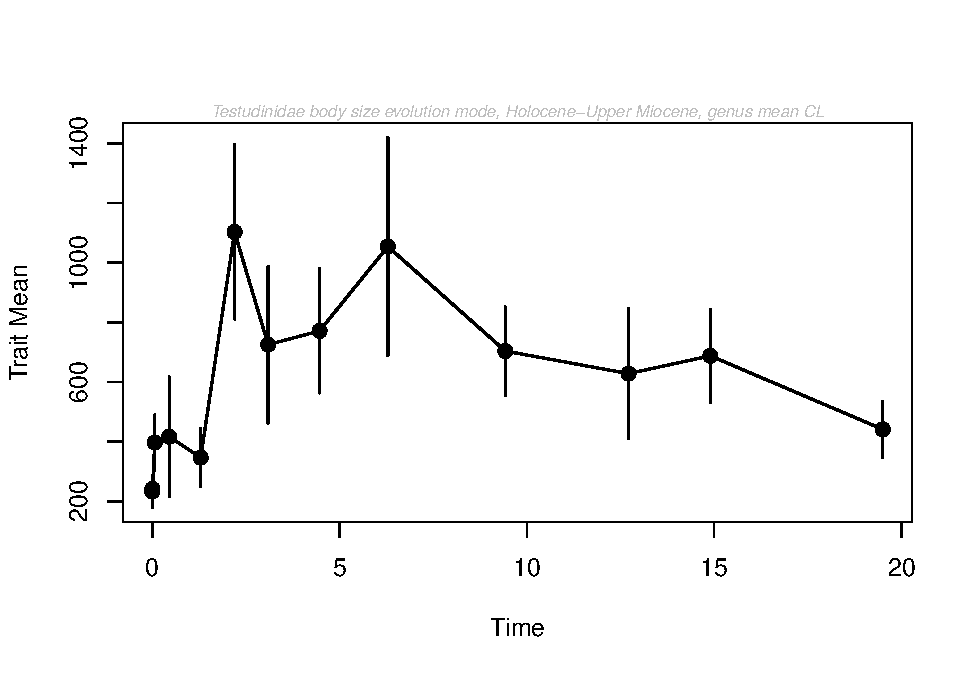
\includegraphics{MA_JJ_files/figure-latex/paleoTSC-1.pdf}
\caption{paleoTS plot with genus mean, continental}
\end{figure}

\begin{longtable}[]{@{}lrrrr@{}}
\caption{Model-fitting results for testudinidae, genera,
continental}\tabularnewline
\toprule
& logL & K & AICc & Akaike.wt\tabularnewline
\midrule
\endfirsthead
\toprule
& logL & K & AICc & Akaike.wt\tabularnewline
\midrule
\endhead
GRW & -82.26287 & 2 & 169.8591 & 0.300\tabularnewline
URW & -83.12577 & 1 & 168.6515 & 0.548\tabularnewline
Stasis & -82.93984 & 2 & 171.2130 & 0.152\tabularnewline
\bottomrule
\end{longtable}

\newpage

\subsection{insular (excluding
continental)}\label{insular-excluding-continental}

\subsubsection{genera (insular)}\label{genera-insular}

\begin{longtable}[]{@{}rrrr@{}}
\caption{paleoTS object, insular}\tabularnewline
\toprule
tt & mm & vv & nn\tabularnewline
\midrule
\endfirsthead
\toprule
tt & mm & vv & nn\tabularnewline
\midrule
\endhead
0.0000005 & 860.9268 & 0.00 & 1\tabularnewline
0.0058500 & 379.5354 & 68570.44 & 12\tabularnewline
0.0688500 & 727.5938 & 14997.58 & 4\tabularnewline
0.4535000 & 748.8333 & 142649.08 & 3\tabularnewline
1.2935000 & 829.6744 & 112964.44 & 6\tabularnewline
2.1970000 & 1178.3333 & 821158.33 & 3\tabularnewline
3.0940000 & 449.4375 & 27058.77 & 4\tabularnewline
4.4660000 & 826.1667 & 15196.06 & 2\tabularnewline
6.2890000 & 1850.0000 & 0.00 & 1\tabularnewline
\bottomrule
\end{longtable}

\begin{figure}[htbp]
\centering
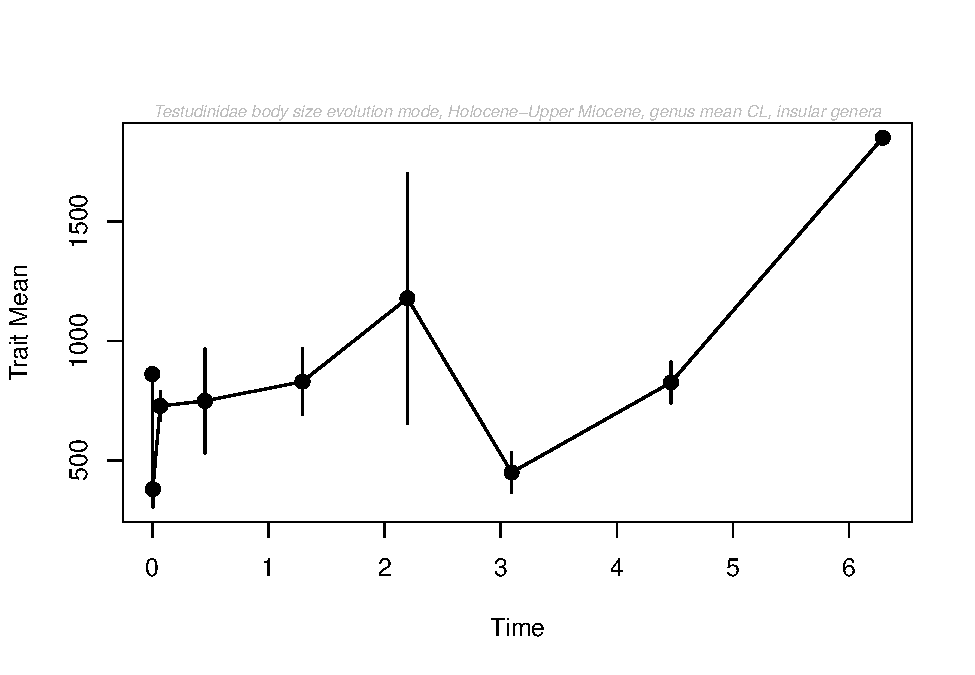
\includegraphics{MA_JJ_files/figure-latex/paleoTSI-1.pdf}
\caption{paleoTS plot with genus mean, insular}
\end{figure}

\begin{longtable}[]{@{}lrrrr@{}}
\caption{Model-fitting results for testudinidae, genera,
insular}\tabularnewline
\toprule
& logL & K & AICc & Akaike.wt\tabularnewline
\midrule
\endfirsthead
\toprule
& logL & K & AICc & Akaike.wt\tabularnewline
\midrule
\endhead
GRW & -68.57344 & 2 & 143.5469 & 0\tabularnewline
URW & -75.76576 & 1 & 154.1982 & 0\tabularnewline
Stasis & -60.41581 & 2 & 127.2316 & 1\tabularnewline
\bottomrule
\end{longtable}

\newpage

\subsection{per continent}\label{per-continent}

\subsubsection{Europe, genera}\label{europe-genera}

\begin{longtable}[]{@{}rrrr@{}}
\caption{paleoTS object, Europe}\tabularnewline
\toprule
mm & nn & vv & tt\tabularnewline
\midrule
\endfirsthead
\toprule
mm & nn & vv & tt\tabularnewline
\midrule
\endhead
148.8559 & 2 & 3338.406 & 0.00585\tabularnewline
616.6667 & 3 & 138802.333 & 0.06885\tabularnewline
377.8167 & 3 & 89203.953 & 0.45350\tabularnewline
697.3717 & 5 & 218431.974 & 1.29350\tabularnewline
895.0000 & 2 & 1110050.000 & 2.19700\tabularnewline
453.3333 & 3 & 39433.333 & 3.09400\tabularnewline
1215.8667 & 5 & 159317.256 & 4.46600\tabularnewline
838.3750 & 2 & 875495.281 & 6.28900\tabularnewline
800.0508 & 6 & 263434.389 & 9.42700\tabularnewline
653.9625 & 5 & 351634.528 & 12.71400\tabularnewline
772.0000 & 5 & 223154.375 & 14.89500\tabularnewline
533.8533 & 5 & 183706.682 & 19.50000\tabularnewline
\bottomrule
\end{longtable}

\begin{figure}[htbp]
\centering
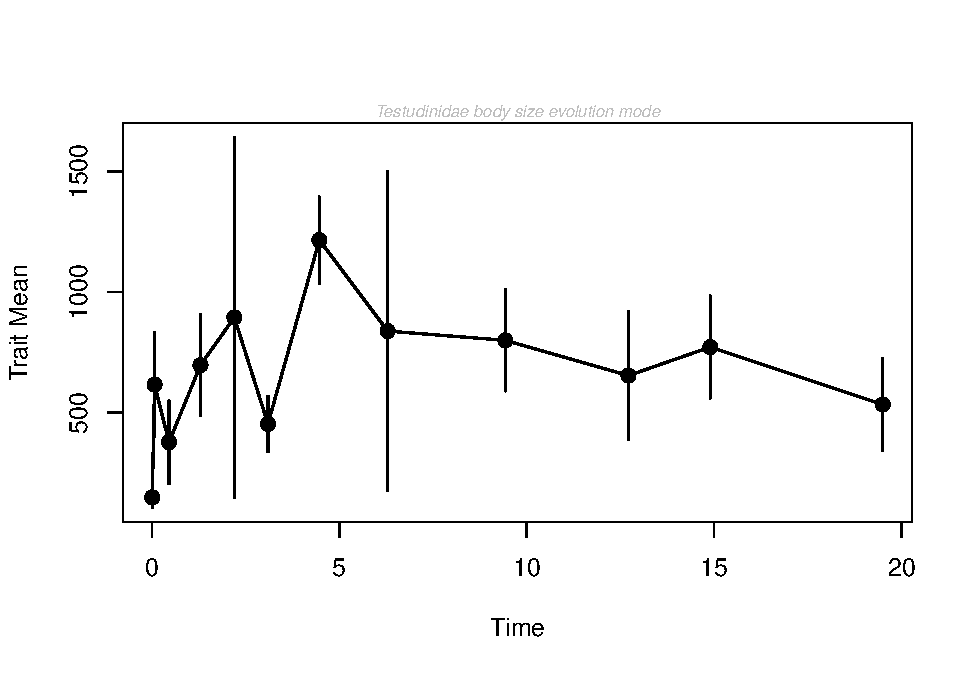
\includegraphics{MA_JJ_files/figure-latex/paleoTSEurope-1.pdf}
\caption{Genera, Europe}
\end{figure}

\begin{longtable}[]{@{}lrrrr@{}}
\caption{Model-fitting results for testudinidae, genera,
Europe}\tabularnewline
\toprule
& logL & K & AICc & Akaike.wt\tabularnewline
\midrule
\endfirsthead
\toprule
& logL & K & AICc & Akaike.wt\tabularnewline
\midrule
\endhead
GRW & -84.14010 & 2 & 173.7802 & 0.006\tabularnewline
URW & -85.90727 & 1 & 174.2590 & 0.005\tabularnewline
Stasis & -79.01365 & 2 & 163.5273 & 0.990\tabularnewline
\bottomrule
\end{longtable}

\newpage

\paragraph{Europe, smaller original bins (see Table 2), genera,
continental}\label{europe-smaller-original-bins-see-table-2-genera-continental}

\begin{longtable}[]{@{}rrrr@{}}
\caption{paleoTs object, Europe, continental}\tabularnewline
\toprule
mm & nn & vv & tt\tabularnewline
\midrule
\endfirsthead
\toprule
mm & nn & vv & tt\tabularnewline
\midrule
\endhead
149.5381 & 2 & 3450.8267 & 0.00585\tabularnewline
187.0000 & 1 & 0.0000 & 0.06885\tabularnewline
205.4750 & 2 & 198.0050 & 0.45350\tabularnewline
204.9292 & 2 & 23.1767 & 1.29350\tabularnewline
1420.0000 & 1 & 0.0000 & 2.19700\tabularnewline
232.5000 & 1 & 0.0000 & 3.09400\tabularnewline
1475.6667 & 3 & 57926.3333 & 4.46600\tabularnewline
663.3750 & 2 & 473607.7812 & 6.28900\tabularnewline
800.0508 & 6 & 263434.3893 & 9.42700\tabularnewline
653.9625 & 5 & 351634.5281 & 12.71400\tabularnewline
772.0000 & 5 & 223154.3750 & 14.89500\tabularnewline
533.8533 & 5 & 183706.6821 & 19.50000\tabularnewline
\bottomrule
\end{longtable}

\begin{figure}[htbp]
\centering
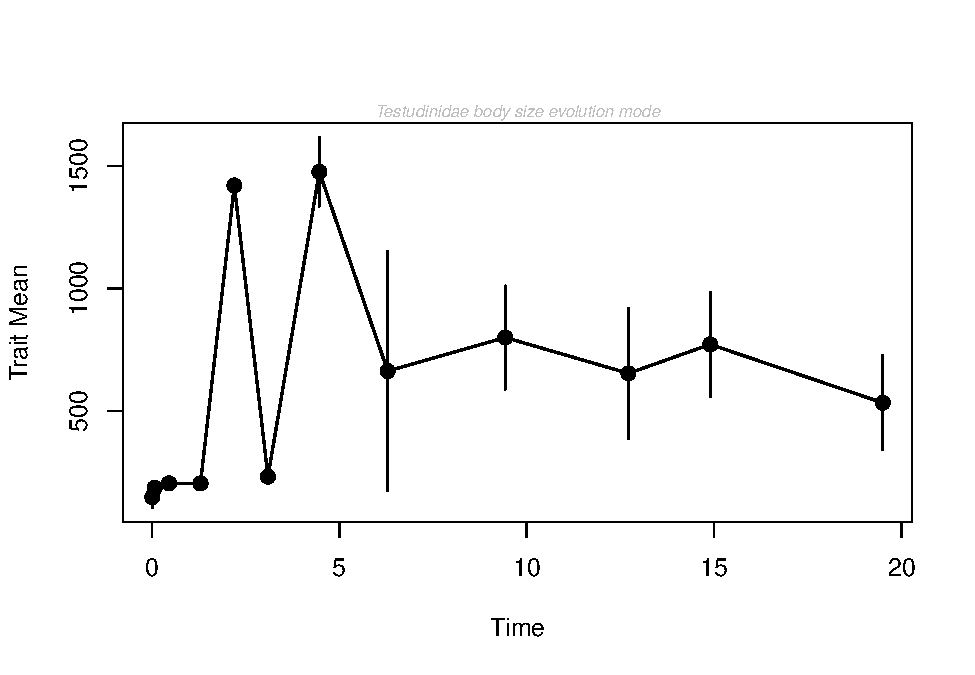
\includegraphics{MA_JJ_files/figure-latex/pTSEuC-1.pdf}
\caption{paleoTS, genera, Europe, continental}
\end{figure}

\begin{longtable}[]{@{}lrrrr@{}}
\caption{Model-fitting results for testudinidae, genera, Europe,
continental}\tabularnewline
\toprule
& logL & K & AICc & Akaike.wt\tabularnewline
\midrule
\endfirsthead
\toprule
& logL & K & AICc & Akaike.wt\tabularnewline
\midrule
\endhead
GRW & -87.93137 & 2 & 181.3627 & 0.009\tabularnewline
URW & -92.56882 & 1 & 187.5821 & 0.000\tabularnewline
Stasis & -83.21073 & 2 & 171.9215 & 0.991\tabularnewline
\bottomrule
\end{longtable}

\newpage

\paragraph{Europe, smaller original bins (see Table 2), genera,
insular}\label{europe-smaller-original-bins-see-table-2-genera-insular}

\begin{longtable}[]{@{}rrrr@{}}
\caption{paleoTs object, Europe, insular}\tabularnewline
\toprule
mm & nn & vv & tt\tabularnewline
\midrule
\endfirsthead
\toprule
mm & nn & vv & tt\tabularnewline
\midrule
\endhead
187.5077 & 1 & 0.00 & 0.00585\tabularnewline
831.5000 & 2 & 684.50 & 0.06885\tabularnewline
722.5000 & 1 & 0.00 & 0.45350\tabularnewline
835.0833 & 4 & 168423.36 & 1.29350\tabularnewline
1005.0000 & 2 & 1462050.00 & 2.19700\tabularnewline
451.6667 & 3 & 40558.33 & 3.09400\tabularnewline
826.1667 & 2 & 15196.06 & 4.46600\tabularnewline
1850.0000 & 1 & 0.00 & 6.28900\tabularnewline
\bottomrule
\end{longtable}

\begin{figure}[htbp]
\centering
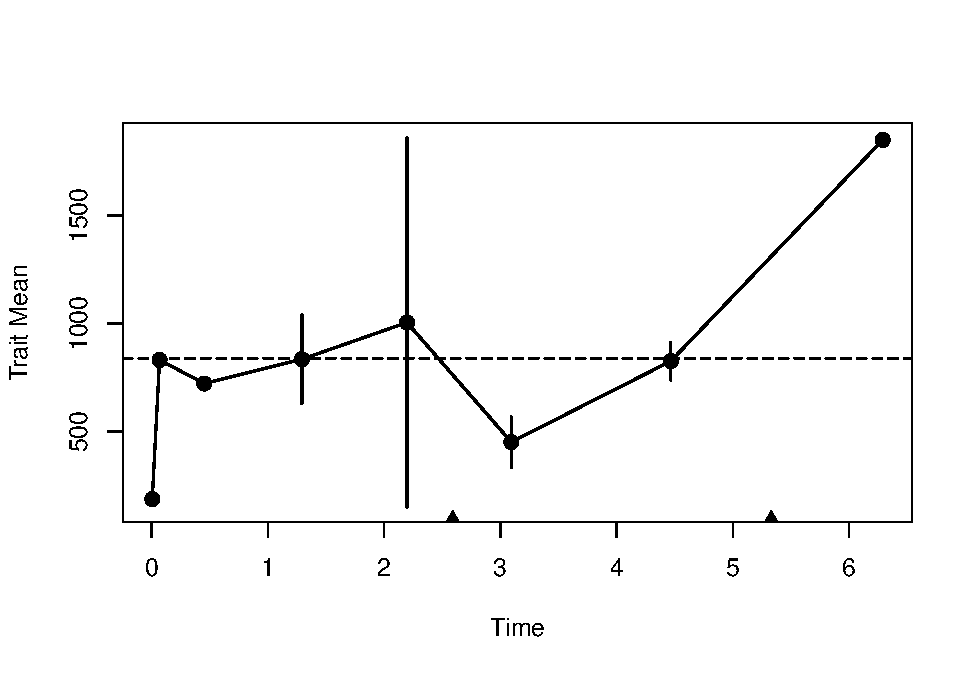
\includegraphics{MA_JJ_files/figure-latex/pTSEuI-1.pdf}
\caption{paleoTS, genera, Europe, insular}
\end{figure}

\begin{longtable}[]{@{}lrrrr@{}}
\caption{Model-fitting results for testudinidae, genera, Europe,
insular}\tabularnewline
\toprule
& logL & K & AICc & Akaike.wt\tabularnewline
\midrule
\endfirsthead
\toprule
& logL & K & AICc & Akaike.wt\tabularnewline
\midrule
\endhead
GRW & -67.12192 & 2 & 141.2438 & 0.000\tabularnewline
URW & -57.51634 & 1 & 117.8327 & 0.074\tabularnewline
Stasis & -52.89638 & 2 & 112.7928 & 0.926\tabularnewline
\bottomrule
\end{longtable}

\newpage 

\subsubsection{Eurasia, smaller original bins (See Table 2),
genera}\label{eurasia-smaller-original-bins-see-table-2-genera}

\begin{longtable}[]{@{}rrrr@{}}
\caption{paleoTS object, Eurasia}\tabularnewline
\toprule
tt & mm & vv & nn\tabularnewline
\midrule
\endfirsthead
\toprule
tt & mm & vv & nn\tabularnewline
\midrule
\endhead
0.0000005 & 137.2637 & 0.000 & 1\tabularnewline
0.0058500 & 236.8217 & 9760.467 & 5\tabularnewline
0.0688500 & 530.0000 & 122579.333 & 4\tabularnewline
0.4535000 & 377.8167 & 89203.953 & 3\tabularnewline
1.2935000 & 777.5579 & 162641.142 & 7\tabularnewline
2.1970000 & 909.6667 & 562217.222 & 5\tabularnewline
3.0940000 & 892.0000 & 381770.000 & 5\tabularnewline
4.4660000 & 1048.0556 & 296417.219 & 6\tabularnewline
6.2890000 & 1208.9167 & 849651.021 & 3\tabularnewline
9.4270000 & 800.0508 & 263434.389 & 6\tabularnewline
12.7140000 & 653.9625 & 351634.528 & 5\tabularnewline
14.8950000 & 772.0000 & 223154.375 & 5\tabularnewline
19.5000000 & 513.8533 & 162399.349 & 5\tabularnewline
\bottomrule
\end{longtable}

\begin{figure}[htbp]
\centering
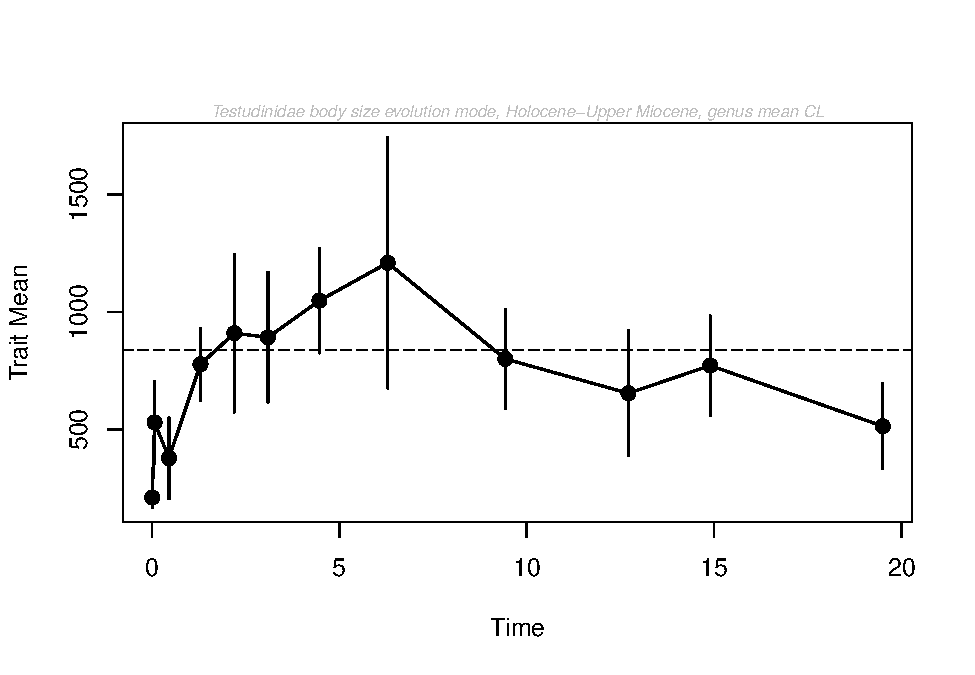
\includegraphics{MA_JJ_files/figure-latex/paleoTSEurasia-1.pdf}
\caption{paleoTS, genera, Eurasia}
\end{figure}

\begin{longtable}[]{@{}lrrrr@{}}
\caption{Model-fitting results for testudinidae, genera,
Eurasia}\tabularnewline
\toprule
& logL & K & AICc & Akaike.wt\tabularnewline
\midrule
\endfirsthead
\toprule
& logL & K & AICc & Akaike.wt\tabularnewline
\midrule
\endhead
GRW & -85.25195 & 2 & 175.8372 & 0.149\tabularnewline
URW & -85.39072 & 1 & 173.1814 & 0.562\tabularnewline
Stasis & -84.58890 & 2 & 174.5111 & 0.289\tabularnewline
\bottomrule
\end{longtable}

\newpage 

\subsubsection{Eurasia, smaller original bins (See Table 2), genera,
continental}\label{eurasia-smaller-original-bins-see-table-2-genera-continental}

\begin{longtable}[]{@{}rrrr@{}}
\caption{paleoTS object, Eurasia, continental}\tabularnewline
\toprule
tt & mm & vv & nn\tabularnewline
\midrule
\endfirsthead
\toprule
tt & mm & vv & nn\tabularnewline
\midrule
\endhead
0.0000005 & 137.2637 & 0.000 & 1\tabularnewline
0.0058500 & 238.0120 & 9654.865 & 5\tabularnewline
0.0688500 & 228.5000 & 3444.500 & 2\tabularnewline
0.4535000 & 205.4750 & 198.005 & 2\tabularnewline
1.2935000 & 595.5388 & 191487.404 & 4\tabularnewline
2.1970000 & 1044.5833 & 442006.250 & 4\tabularnewline
3.0940000 & 1110.8333 & 581102.083 & 3\tabularnewline
4.4660000 & 1159.0000 & 439728.667 & 4\tabularnewline
6.2890000 & 1092.2500 & 788605.188 & 3\tabularnewline
9.4270000 & 800.0508 & 263434.389 & 6\tabularnewline
12.7140000 & 653.9625 & 351634.528 & 5\tabularnewline
14.8950000 & 772.0000 & 223154.375 & 5\tabularnewline
19.5000000 & 513.8533 & 162399.349 & 5\tabularnewline
\bottomrule
\end{longtable}

\begin{figure}[htbp]
\centering
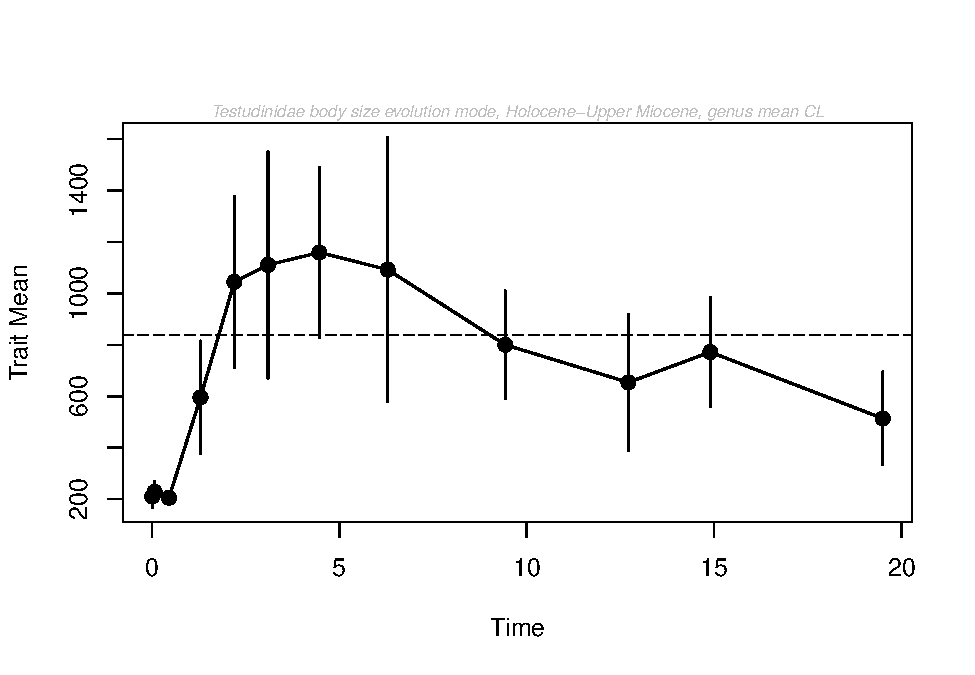
\includegraphics{MA_JJ_files/figure-latex/pTSEsC-1.pdf}
\caption{paleoTS, genera, Eurasia, continental}
\end{figure}

\begin{longtable}[]{@{}lrrrr@{}}
\caption{Model-fitting results for testudinidae, genera, Eurasia,
continental}\tabularnewline
\toprule
& logL & K & AICc & Akaike.wt\tabularnewline
\midrule
\endfirsthead
\toprule
& logL & K & AICc & Akaike.wt\tabularnewline
\midrule
\endhead
GRW & -82.20698 & 2 & 169.7473 & 0.222\tabularnewline
URW & -82.42344 & 1 & 167.2469 & 0.776\tabularnewline
Stasis & -87.19538 & 2 & 179.7241 & 0.002\tabularnewline
\bottomrule
\end{longtable}

\newpage 

\subsubsection{Eurasia, smaller original bins (See Table 2), genera,
insular}\label{eurasia-smaller-original-bins-see-table-2-genera-insular}

\begin{longtable}[]{@{}rrrr@{}}
\caption{paleoTS object, Eurasia, insular}\tabularnewline
\toprule
tt & mm & vv & nn\tabularnewline
\midrule
\endfirsthead
\toprule
tt & mm & vv & nn\tabularnewline
\midrule
\endhead
0.0000005 & 137.2637 & 0.000 & 1\tabularnewline
0.0058500 & 271.4596 & 5668.485 & 4\tabularnewline
0.0688500 & 644.3333 & 105436.333 & 3\tabularnewline
0.4535000 & 722.5000 & 0.000 & 1\tabularnewline
1.2935000 & 882.0356 & 105684.077 & 6\tabularnewline
2.1970000 & 953.6667 & 652233.889 & 5\tabularnewline
3.0940000 & 891.0000 & 383430.000 & 5\tabularnewline
4.4660000 & 620.4444 & 134562.926 & 3\tabularnewline
6.2890000 & 1900.0000 & 5000.000 & 2\tabularnewline
19.5000000 & 800.0000 & 0.000 & 1\tabularnewline
\bottomrule
\end{longtable}

\begin{figure}[htbp]
\centering
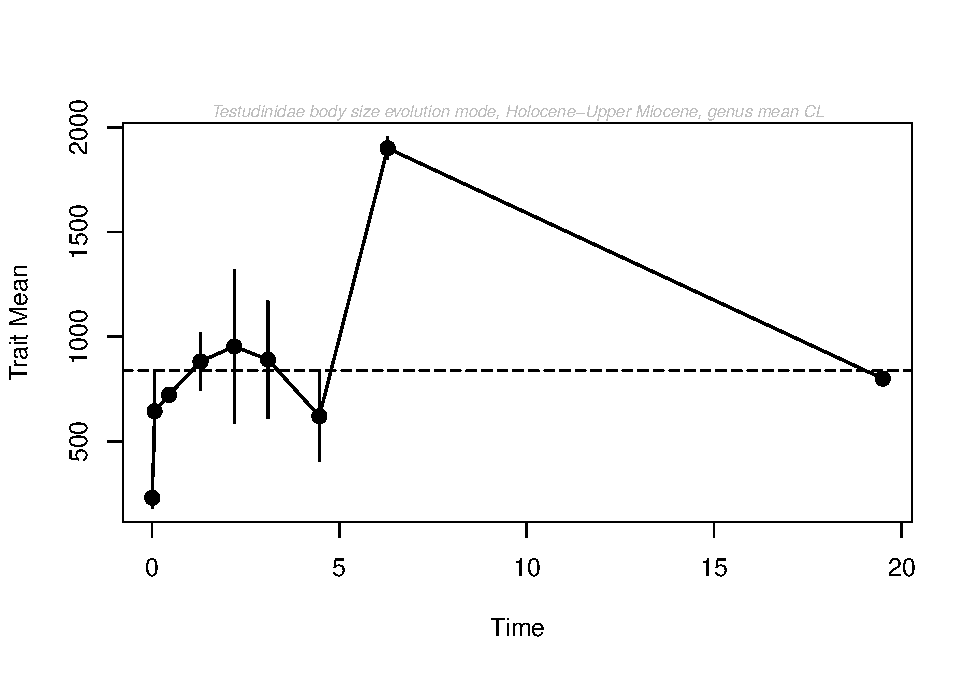
\includegraphics{MA_JJ_files/figure-latex/pTSEsI-1.pdf}
\caption{paleoTS, genera, Eurasia, insular}
\end{figure}

\begin{longtable}[]{@{}lrrrr@{}}
\caption{Model-fitting results for testudinidae, genera, Eurasia,
insular}\tabularnewline
\toprule
& logL & K & AICc & Akaike.wt\tabularnewline
\midrule
\endfirsthead
\toprule
& logL & K & AICc & Akaike.wt\tabularnewline
\midrule
\endhead
GRW & -69.56419 & 2 & 145.1284 & 0.193\tabularnewline
URW & -71.67437 & 1 & 145.9202 & 0.130\tabularnewline
Stasis & -68.31026 & 2 & 142.6205 & 0.677\tabularnewline
\bottomrule
\end{longtable}

\begin{longtable}[]{@{}llrllrll@{}}
\caption{Data set, fossil.}\tabularnewline
\toprule
Genus & Taxon & CL & estimated & EpochBins & Age & Island &
Con\tabularnewline
\midrule
\endfirsthead
\toprule
Genus & Taxon & CL & estimated & EpochBins & Age & Island &
Con\tabularnewline
\midrule
\endhead
Homopus & Homopus aerolatus & 88.00 & m & Modern & 0.000001 & n &
Africa\tabularnewline
Chersina & Chersina angulata & 120.00 & m & Modern & 0.000001 & n &
Africa\tabularnewline
Aldabrachelys & Aldabrachelys gigantea & 870.00 & m & Modern & 0.000001
& y & Africa\tabularnewline
Chersina & Chersina angulata & 170.00 & m & Modern & 0.000001 & n &
Africa\tabularnewline
Indotestudo & Indotestudo travancorica & 224.00 & m & Modern & 0.000001
& n & Africa\tabularnewline
Cylindraspis & Cylindraspis vosmaeri & 500.00 & m & Modern & 0.000001 &
y & Africa\tabularnewline
Centrochelys & Centrochelys sulcata & 435.00 & m & Modern & 0.000001 & n
& Africa\tabularnewline
Kinixys & Kinixys homeana & 193.00 & m & Modern & 0.000001 & n &
Africa\tabularnewline
Stigmochelys & Stigmochelys pardalis & 315.00 & m & Modern & 0.000001 &
n & Africa\tabularnewline
Kinixys & Kinixys belliana & 180.00 & m & Modern & 0.000001 & n &
Africa\tabularnewline
Testudo & Testudo kenitrensis & 132.00 & mo & Middle Pleistocene &
0.453500 & n & Africa\tabularnewline
Cylindraspis & Cylindraspis indica & 600.00 & m & Modern & 0.000001 & y
& Africa\tabularnewline
Psammobates & Psammobates geometricus & 92.00 & m & Modern & 0.000001 &
n & Africa\tabularnewline
Aldabrachelys & Aldabrachelys gigantea & 800.00 & m & Modern & 0.000001
& y & Africa\tabularnewline
Cylindraspis & Cylindraspis triserrata & 1100.00 & m & Modern & 0.000001
& y & Africa\tabularnewline
Astrochelys & Astrochelys yniphora & 307.00 & m & Modern & 0.000001 & y
& Africa\tabularnewline
Stigmochelys & Stigmochelys pardalis & 405.00 & m & Modern & 0.000001 &
n & Africa\tabularnewline
Astrochelys & Astrochelys radiata & 334.00 & m & Modern & 0.000001 & y &
Africa\tabularnewline
Stigmochelys & Stigmochelys pardalis & 297.00 & m & Modern & 0.000001 &
n & Africa\tabularnewline
Astrochelys & Astrochelys radiata & 285.00 & m & Modern & 0.000001 & y &
Africa\tabularnewline
Testudo & Testudo sp. & 200.00 & mf & Gelasian & 2.500000 & n &
Africa\tabularnewline
Astrochelys & Astrochelys radiata & 242.00 & m & Modern & 0.000001 & y &
Africa\tabularnewline
Astrochelys & Astrochelys radiata & 355.00 & m & Modern & 0.000001 & y &
Africa\tabularnewline
Pyxis & Pyxis planicauda & 126.00 & m & Modern & 0.000001 & y &
Africa\tabularnewline
Homopus & Homopus aerolatus & 300.00 & m & Modern & 0.000001 & n &
Africa\tabularnewline
Aldabrachelys & Aldabrachelys gigantea & 770.00 & m & Modern & 0.000001
& y & Africa\tabularnewline
Aldabrachelys & Aldabrachelys gigantea & 720.00 & m & Modern & 0.000001
& y & Africa\tabularnewline
Centrochelys & Centrochelys sulcata & 215.00 & m & Modern & 0.000001 & n
& Africa\tabularnewline
Homopus & Homopus solus & 109.00 & m & Modern & 0.000001 & n &
Africa\tabularnewline
Psammobates & Psammobates oculifer & 101.00 & m & Modern & 0.000001 & n
& Africa\tabularnewline
Homopus & Homopus signatus & 94.00 & m & Modern & 0.000001 & n &
Africa\tabularnewline
Kinixys & Kinixys belliana & 194.00 & m & Modern & 0.000001 & n &
Africa\tabularnewline
Kinixys & Kinixys belliana & 230.00 & m & Modern & 0.000001 & n &
Africa\tabularnewline
Kinixys & Kinixys belliana & 174.00 & m & Modern & 0.000001 & n &
Africa\tabularnewline
Psammobates & Psammobates geometricus & 107.00 & m & Modern & 0.000001 &
n & Africa\tabularnewline
Kinixys & Kinixys lobatsiana & 200.00 & m & Modern & 0.000001 & n &
Africa\tabularnewline
Kinixys & Kinixys natalensis & 160.00 & m & Modern & 0.000001 & n &
Africa\tabularnewline
Chersina & Chersina angulata & 202.00 & m & Modern & 0.000001 & n &
Africa\tabularnewline
Chersina & Chersina angulata & 351.00 & m & Modern & 0.000001 & y &
Africa\tabularnewline
Aldabrachelys & Aldabrachelys gigantea & 1030.00 & m & Modern & 0.000001
& y & Africa\tabularnewline
Chersina & Chersina angulata & 160.00 & m & Modern & 0.000001 & n &
Africa\tabularnewline
Chersina & Chersina angulata & 148.00 & m & Modern & 0.000001 & n &
Africa\tabularnewline
Chersina & Chersina angulata & 181.00 & m & Modern & 0.000001 & n &
Africa\tabularnewline
Psammobates & Psammobates tentorius & 145.00 & m & Modern & 0.000001 & n
& Africa\tabularnewline
Pyxis & Pyxis arachnoides & 150.00 & m & Modern & 0.000001 & y &
Africa\tabularnewline
Pyxis & Pyxis planicauda & 160.00 & m & Modern & 0.000001 & y &
Africa\tabularnewline
Stigmochelys & Stigmochelys pardalis & 720.00 & m & Modern & 0.000001 &
n & Africa\tabularnewline
Malacochersus & Malacochersus tornieri & 153.00 & m & Modern & 0.000001
& n & Africa\tabularnewline
Chersina & Chersina angulata & 179.30 & m & Modern & 0.000001 & n &
Africa\tabularnewline
Aldabrachelys & Aldabrachelys gigantea & 810.00 & m & Modern & 0.000001
& y & Africa\tabularnewline
Testudo & Testudo kleinmanni & 144.00 & m & Modern & 0.000001 & n &
Africa\tabularnewline
Astrochelys & Astrochelys yniphora & 415.00 & m & Modern & 0.000001 & y
& Africa\tabularnewline
Cylindraspis & Cylindraspis inepta & 1000.00 & m & Modern & 0.000001 & y
& Africa\tabularnewline
Cylindraspis & Cylindraspis peltastes & 420.00 & m & Modern & 0.000001 &
y & Africa\tabularnewline
Astrochelys & Astrochelys yniphora & 486.00 & m & Modern & 0.000001 & y
& Africa\tabularnewline
Pyxis & Pyxis planicauda & 148.00 & m & Modern & 0.000001 & y &
Africa\tabularnewline
Astrochelys & Astrochelys yniphora & 426.00 & m & Modern & 0.000001 & y
& Africa\tabularnewline
Pyxis & Pyxis arachnoides & 110.00 & m & Modern & 0.000001 & y &
Africa\tabularnewline
Aldabrachelys & ``Aldabrachelys'' laetoliensis & 1000.00 & mo &
Piacencian & 2.703000 & n & Africa\tabularnewline
Centrochelys & Centrochelys sulcata & 830.00 & m & Modern & 0.000001 & n
& Africa\tabularnewline
Homopus & Homopus fenestratus & 90.00 & mo & Piacencian & 3.056500 & n &
Africa\tabularnewline
Astrochelys & Astrochelys radiata & 395.00 & m & Modern & 0.000001 & y &
Africa\tabularnewline
Pyxis & Pyxis arachnoides & 110.00 & m & Modern & 0.000001 & y &
Africa\tabularnewline
Psammobates & Psammobates tentorius & 116.00 & m & Modern & 0.000001 & y
& Africa\tabularnewline
Pyxis & Pyxis planicauda & 132.00 & m & Modern & 0.000001 & y &
Africa\tabularnewline
Pyxis & Pyxis planicauda & 114.00 & m & Modern & 0.000001 & y &
Africa\tabularnewline
Pyxis & Pyxis planicauda & 134.00 & m & Modern & 0.000001 & y &
Africa\tabularnewline
Homopus & Homopus signatus & 106.00 & m & Modern & 0.000001 & n &
Africa\tabularnewline
Kinixys & Kinixys erosa & 164.00 & m & Modern & 0.000001 & n &
Africa\tabularnewline
Pyxis & Pyxis arachnoides & 111.00 & m & Modern & 0.000001 & y &
Africa\tabularnewline
Mesocherus & Mesocherus orangeus & 180.00 & mo & Burdigalian/Aquitanian
& 17.250000 & n & Africa\tabularnewline
Pyxis & Pyxis arachnoides & 80.00 & m & Modern & 0.000001 & y &
Africa\tabularnewline
Pyxis & Pyxis arachnoides & 144.00 & m & Modern & 0.000001 & y &
Africa\tabularnewline
Kinixys & Kinixys erosa & 400.00 & m & Modern & 0.000001 & n &
Africa\tabularnewline
Kinixys & Kinixys homeana & 223.00 & m & Modern & 0.000001 & n &
Africa\tabularnewline
Kinixys & Kinixys belliana & 157.00 & m & Modern & 0.000001 & n &
Africa\tabularnewline
Kinixys & Kinixys belliana & 162.00 & m & Modern & 0.000001 & n &
Africa\tabularnewline
Chersina & Chersina angulata & 166.40 & m & Modern & 0.000001 & n &
Africa\tabularnewline
Chersina & Chersina angulata & 171.60 & m & Modern & 0.000001 & y &
Africa\tabularnewline
Chersina & Chersina angulata & 136.00 & m & Modern & 0.000001 & n &
Africa\tabularnewline
Mesocherus & Mesocherus orangeus & 180.00 & mo & Burdigalian/Aquitanian
& 17.250000 & n & Africa\tabularnewline
Chersina & Chersina angulata & 161.30 & m & Modern & 0.000001 & y &
Africa\tabularnewline
Kinixys & Kinixys erosa & 271.00 & m & Modern & 0.000001 & n &
Africa\tabularnewline
Psammobates & Psammobates oculifer & 111.00 & m & Modern & 0.000001 & n
& Africa\tabularnewline
Namibchersus & Namibchersus aff. namaquensis & 550.00 & mo &
Burdigalian/Aquitanian & 17.250000 & n & Africa\tabularnewline
Astrochelys & Astrochelys radiata & 305.00 & m & Modern & 0.000001 & y &
Africa\tabularnewline
Impregnochelys & Impregnochelys pachytectis & 620.00 & m &
Burdigalian/Aquitanian & 19.500000 & n & Africa\tabularnewline
Stigmochelys & Stigmochelys pardalis & 345.00 & m & Modern & 0.000001 &
n & Africa\tabularnewline
Stigmochelys & Stigmochelys pardalis & 350.00 & m & Modern & 0.000001 &
n & Africa\tabularnewline
Aldabrachelys & Aldabrachelys gigantea & 875.00 & m & Modern & 0.000001
& y & Africa\tabularnewline
Namibchersus & Namibchersus aff. namaquensis & 1100.00 & mo &
Burdigalian/Aquitanian & 17.250000 & n & Africa\tabularnewline
Geochelone & Geochelone sp. & 1446.00 & eh & Tortonian & 8.476000 & n &
Africa\tabularnewline
Testudo & Testudo sp. & 184.00 & mf & Gelasian & 2.500000 & n &
Africa\tabularnewline
Chersina & Chersina angulata & 153.50 & m & Modern & 0.000001 & n &
Africa\tabularnewline
Psammobates & Psammobates oculifer & 119.00 & m & Modern & 0.000001 & n
& Africa\tabularnewline
Psammobates & Psammobates oculifer & 107.00 & m & Modern & 0.000001 & n
& Africa\tabularnewline
Psammobates & Psammobates geometricus & 165.00 & m & Modern & 0.000001 &
n & Africa\tabularnewline
Aldabrachelys & Aldabrachelys grandidieri & 1250.00 & mo & Modern &
0.001500 & y & Africa\tabularnewline
Psammobates & Psammobates oculifer & 103.00 & m & Modern & 0.000001 & n
& Africa\tabularnewline
Centrochelys & Centrochelys atlantica & 400.00 & mo & Lower Pleistocene
& 1.300000 & y & Africa\tabularnewline
Pyxis & Pyxis arachnoides & 86.00 & m & Modern & 0.000001 & y &
Africa\tabularnewline
Pyxis & Pyxis arachnoides & 154.00 & m & Modern & 0.000001 & y &
Africa\tabularnewline
Psammobates & Psammobates geometricus & 118.00 & m & Modern & 0.000001 &
n & Africa\tabularnewline
Aldabrachelys & Aldabrachelys gigantea & 1190.00 & m & Modern & 0.000001
& y & Africa\tabularnewline
Psammobates & Psammobates tentorius & 95.00 & m & Modern & 0.000001 & n
& Africa\tabularnewline
Psammobates & Psammobates tentorius & 81.00 & m & Modern & 0.000001 & n
& Africa\tabularnewline
Psammobates & Psammobates tentorius & 111.00 & m & Modern & 0.000001 & n
& Africa\tabularnewline
Astrochelys & Astrochelys yniphora & 370.00 & m & Modern & 0.000001 & y
& Africa\tabularnewline
Testudo & Testudo aff. kenitrensis & 142.00 & mf & Gelasian & 2.500000 &
n & Africa\tabularnewline
Pyxis & Pyxis planicauda & 120.00 & m & Modern & 0.000001 & y &
Africa\tabularnewline
Psammobates & Psammobates oculifer & 147.00 & m & Modern & 0.000001 & n
& Africa\tabularnewline
Namibchersus & Namibchersus namaquensis & 815.00 & m &
Burdigalian/Aquitanian & 18.000000 & n & Africa\tabularnewline
Psammobates & Psammobates oculifer & 105.00 & m & Modern & 0.000001 & n
& Africa\tabularnewline
Kinixys & Kinixys sp. & 268.00 & ef & Modern & 0.009500 & n &
Africa\tabularnewline
Aldabrachelys & Aldabrachelys grandidieri & 1240.00 & m & Modern &
0.001500 & y & Africa\tabularnewline
Namibchersus & Namibchersus namaquensis & 264.00 & m &
Burdigalian/Aquitanian & 19.500000 & n & Africa\tabularnewline
Psammobates & Psammobates geometricus & 105.00 & m & Modern & 0.000001 &
n & Africa\tabularnewline
Chersina & Chersina angulata & 162.00 & m & Modern & 0.000001 & n &
Africa\tabularnewline
Astrochelys & Astrochelys radiata & 400.00 & m & Modern & 0.000001 & y &
Africa\tabularnewline
Astrochelys & Astrochelys yniphora & 446.00 & m & Modern & 0.000001 & y
& Africa\tabularnewline
Homopus & Homopus boulengeri & 110.00 & m & Modern & 0.000001 & n &
Africa\tabularnewline
Astrochelys & Astrochelys yniphora & 361.00 & m & Modern & 0.000001 & y
& Africa\tabularnewline
Aldabrachelys & Aldabrachelys abrupta & 1000.00 & mo & Modern & 0.002000
& y & Africa\tabularnewline
Namibchersus & Namibchersus namaquensis & 470.00 & m &
Burdigalian/Aquitanian & 18.000000 & n & Africa\tabularnewline
Namibchersus & Namibchersus namaquensis & 254.00 & m &
Burdigalian/Aquitanian & 18.000000 & n & Africa\tabularnewline
Namibchersus & Namibchersus aff. namaquensis & 440.00 & mo &
Burdigalian/Aquitanian & 17.250000 & n & Africa\tabularnewline
Mesocherus & Mesocherus orangeus & 200.00 & mo & Burdigalian/Aquitanian
& 17.250000 & n & Africa\tabularnewline
Testudo & Testudo oughlamensis & 120.00 & mo & Gelasian & 2.500000 & n &
Africa\tabularnewline
Geochelone & Geochelone stromeri & 425.00 & m & Zanclean & 4.466000 & n
& Africa\tabularnewline
Mesocherus & Mesocherus orangeus & 180.00 & mo & Burdigalian/Aquitanian
& 17.250000 & n & Africa\tabularnewline
Chersina & Chersina angulata & 181.90 & m & Modern & 0.000001 & y &
Africa\tabularnewline
Geochelone & Geochelone stromeri & 350.00 & m & Zanclean & 4.466000 & n
& Africa\tabularnewline
Mesocherus & Mesocherus orangeus & 160.00 & mo & Burdigalian/Aquitanian
& 17.250000 & n & Africa\tabularnewline
Malacochersus & Malacochersus tornieri & 180.00 & m & Modern & 0.000001
& n & Africa\tabularnewline
Homopus & Homopus femoralis & 168.00 & m & Modern & 0.000001 & n &
Africa\tabularnewline
Centrochelys & Centrochelys marocana & 2050.00 & mo & Gelasian &
2.500000 & n & Africa\tabularnewline
Kinixys & Kinixys spekii & 220.00 & m & Modern & 0.000001 & n &
Africa\tabularnewline
Psammobates & Psammobates antiquorum & 107.80 & m & Lower Pleistocene &
1.800000 & n & Africa\tabularnewline
Geochelone & Geochelone crassa & 865.00 & mf & Zanclean & 4.145000 & n &
Africa\tabularnewline
Namibchersus & Namibchersus namaquensis & 470.00 & m &
Burdigalian/Aquitanian & 18.000000 & n & Africa\tabularnewline
Namibchersus & Namibchersus namaquensis & 300.00 & m &
Burdigalian/Aquitanian & 19.500000 & n & Africa\tabularnewline
Aldabrachelys & Aldabrachelys gigantea & 1140.00 & m & Modern & 0.000001
& y & Africa\tabularnewline
Geochelone & Geochelone elegans & 208.00 & m & Modern & 0.000001 & n &
Asia\tabularnewline
Geochelone & Geochelone elegans & 245.00 & m & Modern & 0.000001 & n &
Asia\tabularnewline
Geochelone & Geochelone elegans & 221.00 & m & Modern & 0.000001 & n &
Asia\tabularnewline
Geochelone & Geochelone elegans & 220.00 & m & Modern & 0.000001 & y &
Asia\tabularnewline
Geochelone & Geochelone elegans & 221.00 & m & Modern & 0.000001 & n &
Asia\tabularnewline
Geochelone & Geochelone platynota & 222.00 & m & Modern & 0.000001 & n &
Asia\tabularnewline
Indotestudo & Indotestudo forstenii & 202.00 & m & Modern & 0.000001 & y
& Asia\tabularnewline
Indotestudo & Indotestudo travancorica & 249.70 & m & Modern & 0.000001
& n & Asia\tabularnewline
Indotestudo & Indotestudo forstenii & 309.00 & m & Modern & 0.000001 & y
& Asia\tabularnewline
Aldabrachelys & Aldabrachelys ? sp. & 1500.00 & mo & Piacencian &
3.000000 & n & Asia\tabularnewline
Indotestudo & Indotestudo forstenii & 199.00 & m & Modern & 0.000001 & y
& Asia\tabularnewline
Indotestudo & Indotestudo elongata & 244.20 & m & Modern & 0.000001 & n
& Asia\tabularnewline
Indotestudo & Indotestudo travancorica & 244.20 & m & Modern & 0.000001
& n & Asia\tabularnewline
gen. & gen. indet. & 900.00 & mo & Lower Pleistocene & 1.684500 & n &
Asia\tabularnewline
Testudo & Testudo changshanesis & 330.00 & mo & Lower Pleistocene &
1.684500 & n & Asia\tabularnewline
Indotestudo & Indotestudo elongata & 276.00 & m & Modern & 0.000001 & n
& Asia\tabularnewline
Indotestudo & Indotestudo elongata & 235.00 & m & Modern & 0.000001 & n
& Asia\tabularnewline
Indotestudo & Indotestudo elongata & 208.00 & m & Modern & 0.000001 & n
& Asia\tabularnewline
Indotestudo & Indotestudo elongata & 166.00 & m & Modern & 0.000001 & n
& Asia\tabularnewline
Geochelone & Geochelone sp. & 800.00 & ev & Burdigalian/Aquitanian &
16.500000 & n & Asia\tabularnewline
Megalochelys & Megalochelys sp. & 1200.00 & ev & Lower Pleistocene &
0.900000 & y & Asia\tabularnewline
Testudo & Testudo graeca & 280.00 & m & Modern & 0.000001 & y &
Asia\tabularnewline
Manouria & Manouria emys & 212.00 & m & Modern & 0.000001 & n &
Asia\tabularnewline
Manouria & Manouria emys & 445.00 & m & Modern & 0.000001 & n &
Asia\tabularnewline
Manouria & Manouria emys & 330.00 & m & Modern & 0.000001 & n &
Asia\tabularnewline
Ergilemys & Ergilemys oskarkuhni & 198.00 & m & Zanclean & 3.950000 & n
& Asia\tabularnewline
Testudo & Testudo transcaucasia & 150.00 & mo & Gelasian & 2.190500 & n
& Asia\tabularnewline
Manouria & Manouria impressa & 165.00 & m & Modern & 0.000001 & n &
Asia\tabularnewline
Testudo & Testudo horsfieldii & 280.00 & m & Modern & 0.000001 & n &
Asia\tabularnewline
Indotestudo & Indotestudo travancorica & 219.60 & m & Modern & 0.000001
& n & Asia\tabularnewline
Aldabrachelys & Aldabrachelys ? sp. & 1500.00 & mo & Piacencian &
3.000000 & n & Asia\tabularnewline
Manouria & Manouria emys & 600.00 & m & Modern & 0.000001 & n &
Asia\tabularnewline
Manouria & Manouria impressa & 275.00 & m & Modern & 0.000001 & n &
Asia\tabularnewline
Megalochelys & Megalochelys sondaari & 1000.00 & ec & Lower Pleistocene
& 1.350000 & y & Asia\tabularnewline
Testudo & Testudo graeca & 250.00 & m & Modern & 0.000001 & n &
Asia\tabularnewline
Megalochelys & Megalochelys sp. & 191.40 & m & Lower Pleistocene &
1.684500 & y & Asia\tabularnewline
Geochelone & Geochelone platynota & 300.00 & m & Modern & 0.000001 & n &
Asia\tabularnewline
Megalochelys & Megalochelys atlas & 1400.00 & mo & Gelasian & 2.000000 &
y & Asia\tabularnewline
Indotestudo & Indotestudo elongata & 270.00 & m & Upper Pleistocene &
0.037000 & n & Asia\tabularnewline
Manouria & Manouria oyamai & 450.00 & mo & Modern & 0.011000 & y &
Asia\tabularnewline
Indotestudo & Indotestudo forstenii & 200.50 & m & Modern & 0.000001 & y
& Asia\tabularnewline
Indotestudo & Indotestudo elongata & 219.60 & m & Modern & 0.000001 & n
& Asia\tabularnewline
Ergilemys & Ergilemys oskarkuhni & 220.00 & m & Zanclean & 3.950000 & n
& Asia\tabularnewline
Testudo & Testudo ranovi & 200.00 & mo & Gelasian & 2.190500 & n &
Asia\tabularnewline
Megalochelys & Megalochelys atlas & 1600.00 & mo & Piacencian & 3.094000
& n & Asia\tabularnewline
Megalochelys & Megalochelys atlas & 1600.00 & mo & Piacencian & 3.094000
& n & Asia\tabularnewline
Manouria & Manouria impressa & 350.00 & m & Modern & 0.000001 & n &
Asia\tabularnewline
Megalochelys & Megalochelys sp. & 2000.00 & m & Lower Pleistocene &
1.684500 & y & Asia\tabularnewline
Manouria & Manouria punjabiensis & 900.00 & mo & Gelasian & 2.190500 & n
& Asia\tabularnewline
Indotestudo & Indotestudo elongata & 360.00 & m & Modern & 0.000001 & n
& Asia\tabularnewline
Indotestudo & Indotestudo travancorica & 331.00 & m & Modern & 0.000001
& n & Asia\tabularnewline
Megalochelys & Megalochelys atlas & 1800.00 & m & Messinian & 5.423000 &
n & Asia\tabularnewline
Megalochelys & Megalochelys sondaari & 818.00 & ec & Lower Pleistocene &
1.350000 & y & Asia\tabularnewline
Megalochelys & Megalochelys atlas & 1650.00 & mo & Gelasian & 2.000000 &
y & Asia\tabularnewline
Megalochelys & Megalochelys atlas & 2000.00 & mo & Gelasian & 2.190500 &
n & Asia\tabularnewline
Megalochelys & Megalochelys atlas & 2100.00 & mo & Messinian & 5.423000
& n & Asia\tabularnewline
Manouria & Manouria emys & 600.00 & m & Modern & 0.000001 & n &
Asia\tabularnewline
Geochelone & Geochelone elegans & 380.00 & m & Modern & 0.000001 & n &
Asia\tabularnewline
Testudo & Testudo graeca & 300.00 & m & Modern & 0.000001 & n &
Asia\tabularnewline
Chelonoidis & Chelonoidis marcanoi & 778.00 & eh & Upper Pleistocene &
0.069000 & y & America\tabularnewline
Chelonoidis & Chelonoidis sp. & 440.00 & mo & Modern & 0.001000 & y &
America\tabularnewline
Gopherus & Gopherus morafkai & 299.00 & m & Modern & 0.000001 & n &
America\tabularnewline
Chelonoidis & Chelonoidis alburyorum & 424.00 & m & Piacencian &
3.201500 & y & America\tabularnewline
Chelonoidis & Chelonoidis sp. & 400.00 & mo & Upper Pleistocene &
0.069000 & y & America\tabularnewline
Chelonoidis & Chelonoidis marcanoi & 614.00 & eh & Upper Pleistocene &
0.069000 & y & America\tabularnewline
Gopherus & Gopherus flavomarginatus & 450.00 & m & Lower Pleistocene &
1.050000 & n & America\tabularnewline
Gopherus & Gopherus berlandieri & 256.30 & m & Lower Pleistocene &
1.050000 & n & America\tabularnewline
Chelonoidis & Chelonoidis cubensis & 1139.00 & ef & Middle Pleistocene &
0.393500 & y & America\tabularnewline
Chelonoidis & Chelonoidis monensis & 500.00 & m & Upper Pleistocene &
0.064500 & y & America\tabularnewline
Hesperotestudo & Hesperotestudo sp. & 1500.00 & mo & Lower Pleistocene &
0.966000 & n & America\tabularnewline
Geochelone & Geochelone sp. & 340.00 & mo & Lower Pleistocene & 1.050000
& n & America\tabularnewline
Chelonoidis & Chelonoidis marcanoi & 530.00 & eh & Upper Pleistocene &
0.069000 & y & America\tabularnewline
Gopherus & Gopherus donlaloi & 580.00 & mo & Modern & 0.000175 & n &
America\tabularnewline
Chelonoidis & Chelonoidis sombrerensis & 990.00 & m & Upper Pleistocene
& 0.069000 & y & America\tabularnewline
Chelonoidis & Chelonoidis marcanoi & 767.00 & eh & Upper Pleistocene &
0.069000 & y & America\tabularnewline
Chelonoidis & Chelonoidis alburyorum & 428.00 & m & Piacencian &
3.201500 & y & America\tabularnewline
Chelonoidis & Chelonoidis sp. & 750.00 & mo & Lower Pleistocene &
1.357000 & y & America\tabularnewline
Chelonoidis & Chelonoidis sp. & 600.00 & mo & Lower Pleistocene &
1.357000 & y & America\tabularnewline
Hesperotestudo & Hesperotestudo bermudae & 270.00 & m & Middle
Pleistocene & 0.310000 & y & America\tabularnewline
Chelonoidis & Chelonoidis alburyorum & 453.00 & m & Piacencian &
3.201500 & y & America\tabularnewline
Gopherus & Gopherus flavomarginatus & 400.00 & m & Modern & 0.000001 & n
& America\tabularnewline
Gopherus & Gopherus berlandieri & 240.00 & m & Modern & 0.000001 & n &
America\tabularnewline
Chelonoidis & Chelonoidis sp. & 660.00 & mo & Modern & 0.001000 & y &
America\tabularnewline
Chelonoidis & Chelonoidis sp. & 800.00 & mo & Lower Pleistocene &
1.357000 & y & America\tabularnewline
Chelonoidis & Chelonoidis sp. & 550.00 & mo & Modern & 0.001000 & y &
America\tabularnewline
Chelonoidis & Chelonoidis sp. & 854.00 & mo & Modern & 0.001000 & y &
America\tabularnewline
Chelonoidis & Chelonoidis sp. & 600.00 & mo & Upper Pleistocene &
0.069000 & y & America\tabularnewline
Gopherus & Gopherus berlandieri & 195.00 & m & Lower Pleistocene &
1.050000 & n & America\tabularnewline
Chelonoidis & Chelonoidis alburyorum & 466.00 & m & Piacencian &
3.201500 & y & America\tabularnewline
Hesperotestudo & Hesperotestudo bermudae & 500.00 & m & Middle
Pleistocene & 0.310000 & y & America\tabularnewline
Chelonoidis & Chelonoidis sp. & 512.00 & mo & Modern & 0.001000 & y &
America\tabularnewline
Chelonoidis & Chelonoidis sp. & 550.00 & m & Modern & 0.001000 & y &
America\tabularnewline
Ergilemys & Ergilemys sp. & 1000.00 & m & Langhian & 14.000000 & n &
Europe\tabularnewline
Testudo & Testudo graeca & 195.00 & mf & Lower Pleistocene & 1.770000 &
n & Europe\tabularnewline
Testudo & Testudo hermanni & 138.50 & m & Modern & 0.000001 & n &
Europe\tabularnewline
Testudo & Testudo lunellensis & 194.00 & mf & Middle Pleistocene &
0.450000 & n & Europe\tabularnewline
Titanochelon & Titanochelon bacharidisi & 900.00 & mo & Zanclean &
3.950000 & n & Europe\tabularnewline
Paleotestudo & Paleotestudo antiqua & 183.70 & m & Serravallian &
12.150000 & n & Europe\tabularnewline
Paleotestudo & Paleotestudo antiqua & 229.00 & mf & Serravallian &
13.000000 & n & Europe\tabularnewline
Pyxis & Pyxis arachnoides & 108.00 & m & Modern & 0.000001 & n &
Europe\tabularnewline
Testudo & Testudo hermanni & 145.90 & m & Modern & 0.000001 & y &
Europe\tabularnewline
Titanochelon & Titanochelon sp. & 1420.00 & mo & Gelasian & 1.850000 & n
& Europe\tabularnewline
Centrochelys & Centrochelys robusta & 850.00 & mo & Zanclean & 4.917000
& y & Europe\tabularnewline
Testudo & Testudo marginata & 246.00 & m & Modern & 0.000001 & n &
Europe\tabularnewline
Testudo & Testudo horsfieldii & 114.00 & m & Modern & 0.000001 & n &
Europe\tabularnewline
Cheirogaster & Cheirogaster sp. & 1000.00 & mo & Serravallian &
12.200000 & n & Europe\tabularnewline
Testudo & Testudo graeca & 178.20 & m & Modern & 0.000001 & n &
Europe\tabularnewline
Eurotestudo & Eurotestudo aff. hermanni & 179.30 & mf & Middle
Pleistocene & 0.740000 & n & Europe\tabularnewline
Titanochelon & Titanochelon bacharidisi & 1164.00 & m & Zanclean &
3.950000 & n & Europe\tabularnewline
Testudo & Testudo marginata & 242.50 & m & Modern & 0.000001 & y &
Europe\tabularnewline
Testudo & Testudo hermanni & 130.00 & m & Modern & 0.000001 & n &
Europe\tabularnewline
Testudo & Testudo horsfieldii & 136.00 & m & Modern & 0.000001 & n &
Europe\tabularnewline
Testudo & Testudo graeca & 200.00 & mf & Messinian & 5.500000 & n &
Europe\tabularnewline
Testudo & Testudo kalksburgensis & 225.00 & mo & Burdigalian/Aquitanian
& 18.000000 & n & Europe\tabularnewline
Testudo & Testudo horsfieldii & 132.00 & m & Modern & 0.000001 & n &
Europe\tabularnewline
Testudo & Testudo brevitesta & 165.00 & mf & Piacencian & 2.600000 & n &
Europe\tabularnewline
Testudo & Testudo hermanni & 200.00 & m & Modern & 0.000001 & y &
Europe\tabularnewline
Testudo & Testudo hermanni & 168.30 & m & Modern & 0.000001 & y &
Europe\tabularnewline
Testudo & Testudo marginata & 310.00 & m & Lower Pleistocene & 1.300000
& y & Europe\tabularnewline
Centrochelys & Centrochelys robusta & 1200.00 & ev & Lower Pleistocene &
1.300000 & y & Europe\tabularnewline
Testudo & Testudo graeca & 167.00 & m & Messinian & 5.500000 & n &
Europe\tabularnewline
Eurotestudo & Eurotestudo cf.~hermanni & 150.00 & mo & Gelasian &
2.000000 & y & Europe\tabularnewline
Titanochelon & Titanochelon bacharidisi & 900.00 & mo & Zanclean &
3.950000 & n & Europe\tabularnewline
Testudo & Testudo hermanni & 143.50 & m & Modern & 0.000001 & y &
Europe\tabularnewline
gen. & gen. indet. & 270.00 & mo & Burdigalian/Aquitanian & 16.400000 &
n & Europe\tabularnewline
Testudo & Testudo marginata & 290.00 & m & Modern & 0.000001 & n &
Europe\tabularnewline
Centrochelys & Centrochelys burchardi & 940.00 & mo & Middle Pleistocene
& 0.435000 & y & Europe\tabularnewline
Testudo & Testudo lunellensis & 260.70 & mf & Middle Pleistocene &
0.450000 & n & Europe\tabularnewline
Geochelone & Geochelone s. l. & 1750.00 & mo & Zanclean & 4.466000 & n &
Europe\tabularnewline
Testudo & Testudo marginata & 210.00 & m & Lower Pleistocene & 1.720000
& n & Europe\tabularnewline
Testudo & Testudo hermanni & 183.30 & m & Modern & 0.000001 & y &
Europe\tabularnewline
Testudo & Testudo hermanni & 196.00 & m & Modern & 0.000001 & n &
Europe\tabularnewline
Testudo & Testudo hermanni & 176.90 & m & Modern & 0.000001 & n &
Europe\tabularnewline
Testudo & Testudo graeca & 194.60 & m & Modern & 0.000001 & n &
Europe\tabularnewline
Testudo & Testudo hermanni & 250.00 & m & Modern & 0.000001 & n &
Europe\tabularnewline
Paleotestudo & Paleotestudo sp. & 179.30 & m & Burdigalian/Aquitanian &
16.550000 & n & Europe\tabularnewline
gen. & gen. indet. & 660.00 & m & Tortonian & 8.750000 & n &
Europe\tabularnewline
Testudo & Testudo marginata & 400.00 & m & Modern & 0.000001 & n &
Europe\tabularnewline
Testudo & Testudo hermanni & 176.60 & m & Modern & 0.000001 & y &
Europe\tabularnewline
Testudo & Testudo catalaunica & 232.00 & m & Serravallian & 12.350000 &
n & Europe\tabularnewline
gen. & gen. indet. & 1000.00 & mo & Langhian & 14.700000 & n &
Europe\tabularnewline
Paleotestudo & Paleotestudo sp. & 261.00 & mf & Tortonian & 9.500000 & n
& Europe\tabularnewline
gen. & gen. indet. & 270.00 & mo & Serravallian & 12.200000 & n &
Europe\tabularnewline
Paleotestudo & Paleotestudo antiqua & 275.00 & mf & Langhian & 15.000000
& n & Europe\tabularnewline
Testudo & Testudo horsfieldii & 123.00 & m & Modern & 0.000001 & n &
Europe\tabularnewline
Testudo & Testudo marginata & 242.50 & m & Modern & 0.000001 & y &
Europe\tabularnewline
Testudo & Testudo sp. & 200.00 & mf & Messinian & 6.165000 & n &
Europe\tabularnewline
Cheirogaster & Cheirogaster sp. & 925.00 & ef & Lower Pleistocene &
0.965000 & y & Europe\tabularnewline
Titanochelon & Titanochelon cf.~perpiniana & 1001.00 & mo &
Burdigalian/Aquitanian & 16.370000 & n & Europe\tabularnewline
Testudo & Testudo marginata & 250.00 & m & Modern & 0.000001 & y &
Europe\tabularnewline
Testudo & Testudo lunellensis & 231.00 & ev & Middle Pleistocene &
0.453500 & n & Europe\tabularnewline
Testudo & Testudo sp. & 2500.00 & mf & Zanclean & 3.900000 & n &
Europe\tabularnewline
Centrochelys & Centrochelys burchardi & 500.00 & mo & Middle Pleistocene
& 0.435000 & y & Europe\tabularnewline
Cheirogaster & Cheirogaster sp. & 1170.00 & m & Tortonian & 10.250000 &
n & Europe\tabularnewline
Testudo & Testudo sp. & 1200.00 & mf & Zanclean & 3.960000 & n &
Europe\tabularnewline
Paleotestudo & Paleotestudo antiqua & 145.00 & mf & Serravallian &
13.000000 & n & Europe\tabularnewline
Testudo & Testudo hermanni & 160.00 & m & Modern & 0.000001 & y &
Europe\tabularnewline
Testudo & Testudo hermanni & 157.00 & m & Modern & 0.000001 & y &
Europe\tabularnewline
Eurotestudo & Testudo hermanni & 133.10 & mf & Lower Pleistocene &
1.220000 & n & Europe\tabularnewline
Testudo & Testudo marginata & 246.00 & m & Modern & 0.000001 & n &
Europe\tabularnewline
Testudo & Testudo marginata & 290.00 & m & Lower Pleistocene & 1.300000
& y & Europe\tabularnewline
Testudo & Testudo kalksburgensis & 230.00 & m & Burdigalian/Aquitanian &
19.965000 & n & Europe\tabularnewline
Testudo & Testudo marginata & 246.70 & m & Modern & 0.000001 & n &
Europe\tabularnewline
Testudo & Testudo kalksburgensis & 275.00 & m & Langhian & 14.500000 & n
& Europe\tabularnewline
Testudo & Testudo lunellensis & 176.00 & mo & Middle Pleistocene &
0.453500 & n & Europe\tabularnewline
Paleotestudo & Paleotestudo antiqua & 240.00 & mf & Serravallian &
13.600000 & n & Europe\tabularnewline
Centrochelys & Centrochelys robusta & 1100.00 & mo & Zanclean & 4.917000
& y & Europe\tabularnewline
Testudo & Testudo catalaunica & 107.00 & m & Tortonian & 11.500000 & n &
Europe\tabularnewline
Testudo & Testudo brevitesta & 300.00 & mf & Piacencian & 2.600000 & n &
Europe\tabularnewline
gen. & gen. indet. & 813.00 & ef & Upper Pleistocene & 0.012500 & y &
Europe\tabularnewline
Testudo & Testudo hermanni & 147.00 & m & Modern & 0.000001 & n &
Europe\tabularnewline
Centrochelys & Centrochelys vulcanica & 610.00 & mo & Piacencian &
3.094000 & y & Europe\tabularnewline
Eurotestudo & Eurotestudo hermanni & 170.50 & mf & Middle Pleistocene &
0.600000 & n & Europe\tabularnewline
Testudo & Testudo horsfieldii & 111.00 & m & Modern & 0.000001 & n &
Europe\tabularnewline
Titanochelon & Titanochelon sp. & 520.00 & mo & Piacencian & 2.600000 &
y & Europe\tabularnewline
Paleotestudo & Paleotestudo cf.~sp. & 270.00 & mo & Langhian & 14.700000
& n & Europe\tabularnewline
Testudo & Testudo burgenlandica & 112.00 & m & Tortonian & 8.750000 & n
& Europe\tabularnewline
Testudo & Testudo promarginata & 310.00 & mf & Burdigalian/Aquitanian &
18.000000 & n & Europe\tabularnewline
Centrochelys & Centrochelys burchardi & 800.00 & m & Middle Pleistocene
& 0.435000 & y & Europe\tabularnewline
Testudo & Testudo steinheimensis & 111.00 & m & Serravallian & 12.150000
& n & Europe\tabularnewline
Paleotestudo & Paleotestudo antiqua & 152.00 & m & Serravallian &
13.000000 & n & Europe\tabularnewline
Paleotestudo & Paleotestudo antiqua & 185.00 & mf & Serravallian &
13.000000 & n & Europe\tabularnewline
Titanochelon & Titanochelon bacharidisi & 1196.00 & m & Zanclean &
3.950000 & n & Europe\tabularnewline
gen. & gen. indet. & 880.00 & m & Tortonian & 8.750000 & n &
Europe\tabularnewline
Testudo & Testudo hermanni & 154.00 & m & Modern & 0.000001 & n &
Europe\tabularnewline
Testudo & Testudo hermanni & 173.00 & m & Modern & 0.000001 & y &
Europe\tabularnewline
Testudo & Testudo hermanni & 161.00 & m & Modern & 0.000001 & n &
Europe\tabularnewline
Testudo & Testudo hermanni & 195.00 & m & Modern & 0.000001 & y &
Europe\tabularnewline
Titanochelon & Titanochelon perpiniana & 1140.00 & m & Zanclean &
3.900000 & n & Europe\tabularnewline
Geochelone & Geochelone sp. & 1000.00 & m & Burdigalian/Aquitanian &
16.650000 & n & Europe\tabularnewline
Testudo & Testudo pecorinii & 225.00 & m & Piacencian & 3.094000 & y &
Europe\tabularnewline
Titanochelon & Titanochelon bolivari & 1353.00 & mo & Serravallian &
12.500000 & n & Europe\tabularnewline
Testudo & Testudo cf.~graeca & 185.00 & m & Zanclean & 3.900000 & n &
Europe\tabularnewline
Cheirogaster & Cheirogaster sp. & 1540.00 & ef & Tortonian & 8.300000 &
n & Europe\tabularnewline
Testudo & Testudo sp. & 245.00 & m & Tortonian & 8.300000 & n &
Europe\tabularnewline
Eurotestudo & Eurotestudo globosa & 263.00 & m & Lower Pleistocene &
1.800000 & n & Europe\tabularnewline
Cheirogaster & Cheirogaster sp. & 1500.00 & e & Serravallian & 13.800000
& n & Europe\tabularnewline
Cheirogaster & Cheirogaster gymnesica & 739.00 & ef & Zanclean &
4.450000 & y & Europe\tabularnewline
Paleotestudo & Paleotestudo antiqua & 180.00 & m & Serravallian &
13.000000 & n & Europe\tabularnewline
Paleotestudo & Paleotestudo cf.~sp. & 270.00 & mo & Serravallian &
12.400000 & n & Europe\tabularnewline
Eurotestudo & Eurotestudo hermanni & 237.60 & mf & Middle Pleistocene &
0.600000 & n & Europe\tabularnewline
Eurotestudo & Eurotestudo aff. hermanni & 194.70 & mf & Middle
Pleistocene & 0.740000 & n & Europe\tabularnewline
Titanochelon & Titanochelon schafferi & 2500.00 & mo & Zanclean &
4.466000 & n & Europe\tabularnewline
Paleotestudo & Paleotestudo cf.~antiqua & 113.00 & mf &
Burdigalian/Aquitanian & 17.300000 & n & Europe\tabularnewline
Testudo & Testudo marginata & 241.70 & m & Modern & 0.000001 & n &
Europe\tabularnewline
Titanochelon & Titanochelon bolivari & 1100.00 & mo & Langhian &
15.000000 & n & Europe\tabularnewline
Testudo & Testudo sp. & 245.00 & m & Tortonian & 8.300000 & n &
Europe\tabularnewline
Paleotestudo & Paleotestudo antiqua & 195.00 & mf & Serravallian &
13.000000 & n & Europe\tabularnewline
Testudo & Testudo cf.~promarginata & 250.00 & m & Tortonian & 8.300000 &
n & Europe\tabularnewline
Testudo & Testudo sp. & 245.00 & m & Tortonian & 8.300000 & n &
Europe\tabularnewline
Cheirogaster & Cheirogaster richardi & 1155.00 & mo & Tortonian &
10.400000 & n & Europe\tabularnewline
Centrochelys & Centrochelys burchardi & 650.00 & mo & Middle Pleistocene
& 0.435000 & y & Europe\tabularnewline
Titanochelon & Titanochelon cf.~bolivari & 1600.00 & ef & Langhian &
14.895000 & n & Europe\tabularnewline
Titanochelon & Titanochelon bolivari & 1250.00 & mo & Langhian &
15.000000 & n & Europe\tabularnewline
Titanochelon & Titanochelon cf.~bolivari & 1300.00 & ev & Langhian &
14.895000 & n & Europe\tabularnewline
Paleotestudo & Paleotestudo sp. & 270.00 & mf & Tortonian & 9.500000 & n
& Europe\tabularnewline
Paleotestudo & Paleotestudo antiqua & 159.50 & m & Serravallian &
13.000000 & n & Europe\tabularnewline
Paleotestudo & Paleotestudo antiqua & 213.00 & mf & Serravallian &
13.600000 & n & Europe\tabularnewline
``Hadrianus'' & ``Hadrianus sp.'' & 1000.00 & m & Tortonian & 8.300000 &
n & Europe\tabularnewline
Testudo & Testudo sp. & 245.00 & m & Tortonian & 8.300000 & n &
Europe\tabularnewline
Titanochelon & Titanochelon schafferi & 1850.00 & m & Messinian &
6.250000 & y & Europe\tabularnewline
Paleotestudo & Paleotestudo antiqua & 191.00 & mf & Serravallian &
13.600000 & n & Europe\tabularnewline
Testudo & Testudo amiatae & 140.00 & mo & Messinian & 5.815000 & n &
Europe\tabularnewline
Testudo & Testudo sp. & 245.00 & m & Tortonian & 8.300000 & n &
Europe\tabularnewline
Testudo & Testudo catalaunica & 175.00 & m & Tortonian & 11.500000 & n &
Europe\tabularnewline
Testudo & Testudo rectogularis & 213.00 & mo & Burdigalian/Aquitanian &
16.370000 & n & Europe\tabularnewline
Eurotestudo & Eurotestudo hermanni & 284.00 & mf & Lower Pleistocene &
1.350000 & n & Europe\tabularnewline
Centrochelys & Centrochelys robusta & 600.00 & ev & Lower Pleistocene &
1.300000 & y & Europe\tabularnewline
Paleotestudo & Paleotestudo antiqua & 240.00 & m & Serravallian &
13.000000 & n & Europe\tabularnewline
Testudo & Testudo cf.~promarginata & 250.00 & m & Tortonian & 8.300000 &
n & Europe\tabularnewline
Testudo & Testudo sp. & 500.00 & mo & Zanclean & 3.900000 & n &
Europe\tabularnewline
Testudo & Testudo sp. & 2500.00 & mf & Zanclean & 3.900000 & n &
Europe\tabularnewline
Paleotestudo & Paleotestudo antiqua & 283.80 & mf & Serravallian &
12.500000 & n & Europe\tabularnewline
Paleotestudo & Paleotestudo antiqua & 234.00 & mf & Serravallian &
13.600000 & n & Europe\tabularnewline
Testudo & Testudo cf.~promarginata & 250.00 & m & Tortonian & 8.300000 &
n & Europe\tabularnewline
Testudo & Testudo sp. & 232.10 & m & Tortonian & 10.750000 & n &
Europe\tabularnewline
Titanochelon & Titanochelon bolivari & 1300.00 & mf & Tortonian &
9.500000 & n & Europe\tabularnewline
Paleotestudo & Paleotestudo antiqua & 195.00 & m & Serravallian &
13.000000 & n & Europe\tabularnewline
Testudo & Testudo promarginata & 304.70 & mf & Burdigalian/Aquitanian &
21.500000 & n & Europe\tabularnewline
Titanochelon & Titanochelon aff. schafferi & 1860.00 & m & Gelasian &
2.000000 & y & Europe\tabularnewline
Paleotestudo & Paleotestudo antiqua & 220.00 & mf & Serravallian &
13.000000 & n & Europe\tabularnewline
Paleotestudo & Paleotestudo antiqua & 206.00 & mf & Serravallian &
13.000000 & n & Europe\tabularnewline
Testudo & Testudo promarginata & 230.00 & mf & Burdigalian/Aquitanian &
21.500000 & n & Europe\tabularnewline
Testudo & Testudo hermanni & 220.00 & mf & Lower Pleistocene & 1.300000
& n & Europe\tabularnewline
Testudo & Testudo s. s. & 189.00 & m & Tortonian & 8.000000 & n &
Europe\tabularnewline
Testudo & Testudo sp. & 245.00 & m & Tortonian & 8.300000 & n &
Europe\tabularnewline
Eurotestudo & Eurotestudo hermanni & 126.00 & mf & Lower Pleistocene &
1.150000 & n & Europe\tabularnewline
Centrochelys & Centrochelys robusta & 850.00 & ev & Lower Pleistocene &
1.300000 & y & Europe\tabularnewline
Centrochelys & Centrochelys robusta & 790.00 & ef & Zanclean & 4.917000
& y & Europe\tabularnewline
Eurotestudo & Eurotestudo hermanni & 187.00 & mf & Upper Pleistocene &
0.110500 & n & Europe\tabularnewline
Testudo & Testudo catalaunica & 181.00 & m & Tortonian & 11.500000 & n &
Europe\tabularnewline
Testudo & Testudo steinheimensis & 227.70 & mf & Serravallian &
13.000000 & n & Europe\tabularnewline
Paleotestudo & Paleotestudo sp. & 170.00 & mf & Tortonian & 9.500000 & n
& Europe\tabularnewline
Testudo & Testudo burgenlandica & 275.00 & m & Tortonian & 8.750000 & n
& Europe\tabularnewline
Paleotestudo & Paleotestudo antiqua & 203.00 & m & Serravallian &
12.150000 & n & Europe\tabularnewline
Cheirogaster & Cheirogaster cf.~gymnesica & 789.00 & mo & Lower
Pleistocene & 1.800000 & y & Europe\tabularnewline
gen. & gen. indet. & 440.00 & m & Tortonian & 8.750000 & n &
Europe\tabularnewline
Testudo & Testudo catalaunica & 165.00 & m & Tortonian & 11.500000 & n &
Europe\tabularnewline
Testudo & Testudo graeca & 210.00 & mf & Tortonian & 8.450000 & n &
Europe\tabularnewline
Titanochelon & Titanochelon gymnesica & 1300.00 & ef & Lower Pleistocene
& 1.300000 & y & Europe\tabularnewline
Centrochelys & Centrochelys robusta & 850.00 & mo & Upper Pleistocene &
0.066000 & y & Europe\tabularnewline
Testudo & Testudo cf.~promarginata & 250.00 & m & Tortonian & 8.300000 &
n & Europe\tabularnewline
Titanochelon & Titanochelon cf.~bolivari & 1500.00 & mf & Tortonian &
9.433000 & n & Europe\tabularnewline
Titanochelon & Titanochelon bolivari & 1150.00 & m & Messinian &
6.289000 & n & Europe\tabularnewline
Testudo & Testudo cf.~promarginata & 250.00 & m & Tortonian & 8.300000 &
n & Europe\tabularnewline
Hesperotestudo & Hesperotestudo mlynarskii & 165.00 & m & Lower
Pleistocene & 1.250000 & n & America\tabularnewline
Gopherus & Gopherus agassizi & 252.00 & m & Upper Pleistocene & 0.025500
& n & America\tabularnewline
Gopherus & Gopherus polyphemus & 273.24 & mo & Upper Pleistocene &
0.069000 & n & America\tabularnewline
Gopherus & Gopherus flavomarginatus & 371.00 & m & Modern & 0.000001 & n
& America\tabularnewline
Gopherus & Gopherus polyphemus & 301.97 & mo & Upper Pleistocene &
0.069000 & n & America\tabularnewline
Gopherus & Gopherus polyphemus & 238.90 & m & Modern & 0.000001 & n &
America\tabularnewline
Gopherus & Gopherus polyphemus & 268.80 & m & Modern & 0.000001 & y &
America\tabularnewline
Gopherus & Gopherus sp. & 216.37 & m & Modern & 0.000001 & n &
America\tabularnewline
Hesperotestudo & Hesperotestudo crassiscutata & 180.40 & m & Upper
Pleistocene & 0.069000 & n & America\tabularnewline
Gopherus & Gopherus polyphemus & 102.44 & mo & Upper Pleistocene &
0.069000 & n & America\tabularnewline
Gopherus & Gopherus polyphemus & 308.00 & m & Modern & 0.000001 & n &
America\tabularnewline
Hesperotestudo & Hesperotestudo crassiscutata & 327.00 & m & Lower
Pleistocene & 1.300000 & n & America\tabularnewline
Gopherus & Gopherus polyphemus & 350.00 & mo & Upper Pleistocene &
0.069000 & n & America\tabularnewline
Hesperotestudo & Hesperotestudo crassiscutata & 425.00 & mo & Upper
Pleistocene & 0.012000 & n & America\tabularnewline
Hesperotestudo & Hesperotestudo wilsoni & 226.00 & m & Upper Pleistocene
& 0.018000 & n & America\tabularnewline
Gopherus & Gopherus flavomarginatus & 246.00 & m & Modern & 0.000001 & n
& America\tabularnewline
Gopherus & Gopherus polyphemus & 431.48 & mo & Upper Pleistocene &
0.069000 & n & America\tabularnewline
Hesperotestudo & Hesperotestudo incisa & 216.00 & m & Lower Pleistocene
& 1.300000 & n & America\tabularnewline
Gopherus & Gopherus polyphemus & 303.00 & m & Modern & 0.000001 & y &
America\tabularnewline
Hesperotestudo & Hesperotestudo crassiscutata & 1250.00 & ev & Upper
Pleistocene & 0.012000 & n & America\tabularnewline
Hesperotestudo & Hesperotestudo sp. & 1000.00 & mo & Gelasian & 2.000000
& n & America\tabularnewline
Gopherus & Gopherus polyphemus & 391.90 & mo & Upper Pleistocene &
0.069000 & n & America\tabularnewline
Gopherus & Gopherus polyphemus & 155.50 & mo & Upper Pleistocene &
0.069000 & n & America\tabularnewline
Hesperotestudo & Hesperotestudo crassiscutata & 282.70 & m & Upper
Pleistocene & 0.069000 & n & America\tabularnewline
Gopherus & Gopherus polyphemus & 239.80 & mo & Middle Pleistocene &
0.250000 & n & America\tabularnewline
Hesperotestudo & Hesperotestudo incisa & 224.00 & m & Lower Pleistocene
& 1.300000 & n & America\tabularnewline
Hesperotestudo & Hesperotestudo equicomes & 340.00 & ev & Middle
Pleistocene & 0.300000 & n & America\tabularnewline
Gopherus & Gopherus sp. & 194.90 & mo & Gelasian & 1.900000 & n &
America\tabularnewline
Hesperotestudo & Hesperotestudo incisa & 212.00 & m & Lower Pleistocene
& 1.300000 & n & America\tabularnewline
Hesperotestudo & Hesperotestudo crassiscutata & 180.00 & m & Lower
Pleistocene & 1.300000 & n & America\tabularnewline
Gopherus & Gopherus sp. & 241.56 & m & Modern & 0.000001 & n &
America\tabularnewline
Gopherus & Gopherus polyphemus & 279.94 & mo & Upper Pleistocene &
0.069000 & n & America\tabularnewline
Hesperotestudo & Hesperotestudo crassiscutata & 188.00 & mo & Upper
Pleistocene & 0.012000 & n & America\tabularnewline
Gopherus & Gopherus sp. & 211.31 & m & Modern & 0.000001 & n &
America\tabularnewline
Gopherus & Gopherus polyphemus & 304.70 & mo & Middle Pleistocene &
0.400000 & n & America\tabularnewline
Gopherus & Gopherus polyphemus & 327.60 & mo & Upper Pleistocene &
0.069000 & n & America\tabularnewline
Gopherus & Gopherus sp. & 264.11 & m & Modern & 0.000001 & n &
America\tabularnewline
Gopherus & Gopherus polyphemus & 260.11 & mo & Upper Pleistocene &
0.069000 & n & America\tabularnewline
Gopherus & Gopherus sp. & 259.50 & mo & Lower Pleistocene & 1.800000 & n
& America\tabularnewline
Hesperotestudo & Hesperotestudo incisa & 232.76 & m & Upper Pleistocene
& 0.069000 & n & America\tabularnewline
Hesperotestudo & Hesperotestudo crassiscutata & 284.90 & m & Upper
Pleistocene & 0.069000 & n & America\tabularnewline
Gopherus & Gopherus polyphemus & 302.40 & mo & Upper Pleistocene &
0.069000 & n & America\tabularnewline
Gopherus & Gopherus sp. & 209.60 & mo & Gelasian & 1.900000 & n &
America\tabularnewline
Gopherus & Gopherus polyphemus & 342.00 & m & Modern & 0.000001 & n &
America\tabularnewline
Gopherus & Gopherus polyphemus & 300.00 & m & Modern & 0.000001 & y &
America\tabularnewline
Gopherus & Gopherus polyphemus & 272.48 & mo & Middle Pleistocene &
0.250000 & n & America\tabularnewline
Gopherus & Gopherus polyphemus & 283.41 & mo & Middle Pleistocene &
0.250000 & n & America\tabularnewline
Hesperotestudo & Hesperotestudo sp. & 639.00 & m & Upper Pleistocene &
0.060000 & n & America\tabularnewline
Gopherus & Gopherus sp. & 181.00 & mo & Gelasian & 1.900000 & n &
America\tabularnewline
Gopherus & Gopherus polyphemus & 387.00 & m & Modern & 0.000001 & n &
America\tabularnewline
Gopherus & Gopherus praecedens & 360.00 & mo & Upper Pleistocene &
0.069000 & n & America\tabularnewline
Gopherus & Gopherus polyphemus & 348.70 & mo & Middle Pleistocene &
0.400000 & n & America\tabularnewline
Testudo & Testudo sp. & 400.00 & mo & Langhian & 14.181000 & n &
America\tabularnewline
Hesperotestudo & Hesperotestudo sp. & 1500.00 & mo & Middle Pleistocene
& 0.700000 & n & America\tabularnewline
Gopherus & Gopherus sp. & 204.40 & mo & Gelasian & 1.900000 & n &
America\tabularnewline
Hesperotestudo & Hesperotestudo crassiscutata & 561.00 & m & Lower
Pleistocene & 1.250000 & n & America\tabularnewline
Gopherus & Gopherus polyphemus & 292.00 & mo & Middle Pleistocene &
0.250000 & n & America\tabularnewline
Gopherus & Gopherus sp. & 163.50 & mo & Gelasian & 1.900000 & n &
America\tabularnewline
Hesperotestudo & Hesperotestudo turgida & 230.00 & mo & Lower
Pleistocene & 1.684500 & n & America\tabularnewline
Gopherus & Gopherus flavomarginatus & 222.00 & m & Modern & 0.000001 & n
& America\tabularnewline
Caudochelys & Caudochelys ducateli & 339.90 & m & Langhian & 15.000000 &
n & America\tabularnewline
Gopherus & Gopherus flavomarginatus & 281.00 & m & Modern & 0.000001 & n
& America\tabularnewline
Gopherus & Gopherus polyphemus & 272.57 & mo & Middle Pleistocene &
0.400000 & n & America\tabularnewline
Gopherus & Gopherus polyphemus & 314.60 & mo & Middle Pleistocene &
0.250000 & n & America\tabularnewline
Gopherus & Gopherus polyphemus & 217.90 & mo & Lower Pleistocene &
1.200000 & n & America\tabularnewline
Gopherus & Gopherus polyphemus & 294.16 & mo & Upper Pleistocene &
0.069000 & n & America\tabularnewline
Geochelone & Geochelone sp. & 350.00 & ef & Upper Pleistocene & 0.069000
& n & America\tabularnewline
Gopherus & Gopherus mohavetus & 412.50 & m & Tortonian & 8.476000 & n &
America\tabularnewline
Gopherus & Gopherus sp. & 230.10 & mo & Lower Pleistocene & 1.800000 & n
& America\tabularnewline
Gopherus & Gopherus polyphemus & 334.70 & mo & Upper Pleistocene &
0.069000 & n & America\tabularnewline
Gopherus & Gopherus polyphemus & 285.60 & mo & Middle Pleistocene &
0.400000 & n & America\tabularnewline
Gopherus & Gopherus sp. & 256.08 & m & Modern & 0.000001 & n &
America\tabularnewline
Gopherus & Gopherus mohavetus & 334.50 & m & Tortonian & 8.476000 & n &
America\tabularnewline
Hesperotestudo & Hesperotestudo incisa & 231.00 & m & Lower Pleistocene
& 1.300000 & n & America\tabularnewline
Hesperotestudo & Hesperotestudo incisa & 228.00 & m & Lower Pleistocene
& 1.300000 & n & America\tabularnewline
Gopherus & Gopherus sp. & 118.90 & mo & Gelasian & 1.900000 & n &
America\tabularnewline
Gopherus & Gopherus polyphemus & 304.20 & mo & Upper Pleistocene &
0.069000 & n & America\tabularnewline
Gopherus & Gopherus agassizi & 445.00 & mo & Middle Pleistocene &
0.156000 & n & America\tabularnewline
Gopherus & Gopherus polyphemus & 278.00 & mo & Upper Pleistocene &
0.069000 & n & America\tabularnewline
Caudochelys & Caudochelys rexroadensis & 781.00 & m & Zanclean &
4.550000 & n & America\tabularnewline
Gopherus & Gopherus polyphemus & 252.56 & mo & Upper Pleistocene &
0.069000 & n & America\tabularnewline
Gopherus & Gopherus polyphemus & 284.90 & mo & Upper Pleistocene &
0.069000 & n & America\tabularnewline
Gopherus & Gopherus sp. & 180.90 & mo & Gelasian & 1.900000 & n &
America\tabularnewline
Gopherus & Gopherus polyphemus & 306.00 & mo & Middle Pleistocene &
0.250000 & n & America\tabularnewline
Hesperotestudo & Hesperotestudo crassiscutata & 168.00 & m & Lower
Pleistocene & 1.300000 & n & America\tabularnewline
Hesperotestudo & Hesperotestudo incisa & 241.00 & m & Lower Pleistocene
& 1.300000 & n & America\tabularnewline
Geochelone & Geochelone tedwhitei & 440.00 & m & Burdigalian/Aquitanian
& 18.500000 & n & America\tabularnewline
Gopherus & Gopherus polyphemus & 257.80 & mo & Middle Pleistocene &
0.250000 & n & America\tabularnewline
Hesperotestudo & Hesperotestudo mlynarskii & 203.50 & m & Lower
Pleistocene & 1.250000 & n & America\tabularnewline
Geochelone & Geochelone tedwhitei & 370.00 & m & Burdigalian/Aquitanian
& 18.500000 & n & America\tabularnewline
Caudochelys & Caudochelys williamsi & 334.00 & m &
Burdigalian/Aquitanian & 17.750000 & n & America\tabularnewline
Gopherus & Gopherus polyphemus & 267.00 & mo & Middle Pleistocene &
0.250000 & n & America\tabularnewline
Gopherus & Gopherus pertenuis & 1050.00 & mo & Lower Pleistocene &
1.684500 & n & America\tabularnewline
Hesperotestudo & Hesperotestudo sp. & 974.00 & ep & Upper Pleistocene &
0.060000 & n & America\tabularnewline
Hesperotestudo & Hesperotestudo incisa & 290.40 & m & Lower Pleistocene
& 1.300000 & n & America\tabularnewline
Geochelone & Geochelone sp. & 880.00 & m & Zanclean & 4.500000 & n &
America\tabularnewline
Caudochelys & Caudochelys rexroadensis & 830.00 & m & Zanclean &
4.550000 & n & America\tabularnewline
Hesperotestudo & Hesperotestudo sp. & 176.00 & mf & Piacencian &
3.100000 & n & America\tabularnewline
Hesperotestudo & Hesperotestudo oelrichi & 283.80 & m & Piacencian &
3.000000 & n & America\tabularnewline
Gopherus & Gopherus sp. & 224.10 & mo & Lower Pleistocene & 1.800000 & n
& America\tabularnewline
Hesperotestudo & Hesperotestudo johnstoni & 235.00 & m & Piacencian &
3.350000 & n & America\tabularnewline
Hesperotestudo & Hesperotestudo riggsi & 185.00 & m & Piacencian &
3.000000 & n & America\tabularnewline
Gopherus & Gopherus agassizii & 400.00 & m & Modern & 0.000001 & n &
America\tabularnewline
Gopherus & Gopherus polyphemus & 292.94 & mo & Middle Pleistocene &
0.250000 & n & America\tabularnewline
Hesperotestudo & Hesperotestudo crassiscutata & 192.00 & m & Lower
Pleistocene & 1.300000 & n & America\tabularnewline
Gopherus & Gopherus polyphemus & 258.30 & mo & Upper Pleistocene &
0.069000 & n & America\tabularnewline
Gopherus & Gopherus sp. & 236.70 & mo & Gelasian & 1.900000 & n &
America\tabularnewline
Gopherus & Gopherus sp. & 218.80 & mo & Gelasian & 1.900000 & n &
America\tabularnewline
Hesperotestudo & Hesperotestudo orthopygia & 682.00 & mo & Messinian &
5.500000 & n & America\tabularnewline
Gopherus & Gopherus polyphemus & 293.57 & mo & Middle Pleistocene &
0.400000 & n & America\tabularnewline
Gopherus & Gopherus polyphemus & 302.40 & mo & Middle Pleistocene &
0.250000 & n & America\tabularnewline
Hesperotestudo & Hesperotestudo sp. & 1800.00 & mo & Middle Pleistocene
& 0.700000 & n & America\tabularnewline
Geochelone & Geochelone sp. & 170.00 & mf & Middle Pleistocene &
0.700000 & n & America\tabularnewline
Gopherus & Gopherus canyonensis & 885.50 & m & Piacencian & 2.700000 & n
& America\tabularnewline
Gopherus & Gopherus polyphemus & 276.60 & mo & Lower Pleistocene &
1.200000 & n & America\tabularnewline
Gopherus & Gopherus ? sp. & 500.00 & m & Serravallian & 11.850000 & n &
America\tabularnewline
Hesperotestudo & Hesperotestudo riggsi & 176.00 & m & Piacencian &
3.000000 & n & America\tabularnewline
Gopherus & Gopherus polyphemus & 324.00 & mo & Upper Pleistocene &
0.069000 & n & America\tabularnewline
Geochelone & Geochelone sp. & 600.00 & mo & Upper Pleistocene & 0.012500
& y & America\tabularnewline
Gopherus & Gopherus mohavetus & 315.00 & m & Tortonian & 8.476000 & n &
America\tabularnewline
Gopherus & Gopherus mohavetus & 360.00 & m & Tortonian & 8.476000 & n &
America\tabularnewline
Gopherus & Gopherus polyphemus & 260.51 & mo & Middle Pleistocene &
0.400000 & n & America\tabularnewline
Gopherus & Gopherus polyphemus & 283.00 & mo & Middle Pleistocene &
0.250000 & n & America\tabularnewline
Hesperotestudo & Hesperotestudo campester & 1000.00 & mo & Gelasian &
2.190500 & n & America\tabularnewline
Gopherus & Gopherus polyphemus & 306.00 & mo & Middle Pleistocene &
0.250000 & n & America\tabularnewline
Gopherus & Gopherus polyphemus & 352.00 & mo & Upper Pleistocene &
0.012000 & n & America\tabularnewline
Gopherus & Gopherus sp. & 181.00 & mo & Gelasian & 1.900000 & n &
America\tabularnewline
Gopherus & Gopherus flavomarginatus & 303.00 & m & Modern & 0.000001 & n
& America\tabularnewline
Gopherus & Gopherus polyphemus & 350.83 & mo & Middle Pleistocene &
0.400000 & n & America\tabularnewline
Gopherus & Gopherus laticaudatus & 375.00 & mo & Middle Pleistocene &
0.396350 & n & America\tabularnewline
Gopherus & Gopherus sp. & 188.30 & mo & Gelasian & 1.900000 & n &
America\tabularnewline
Gopherus & Gopherus polyphemus & 285.20 & mo & Middle Pleistocene &
0.250000 & n & America\tabularnewline
Gopherus & Gopherus polyphemus & 308.20 & mo & Middle Pleistocene &
0.400000 & n & America\tabularnewline
Gopherus & Gopherus ? sp. & 500.00 & m & Tortonian & 10.100000 & n &
America\tabularnewline
Gopherus & Gopherus sp. & 143.90 & mo & Gelasian & 1.900000 & n &
America\tabularnewline
Gopherus & Gopherus sp. & 193.30 & mo & Gelasian & 1.900000 & n &
America\tabularnewline
Geochelone & Geochelone sp. & 176.00 & e & Zanclean & 5.000000 & n &
America\tabularnewline
Gopherus & Gopherus sp. & 182.30 & mo & Gelasian & 1.900000 & n &
America\tabularnewline
Hesperotestudo & Hesperotestudo riggsi & 195.80 & m & Zanclean &
4.550000 & n & America\tabularnewline
Hesperotestudo & Hesperotestudo orthopygia & 1200.00 & mo & Messinian &
5.500000 & n & America\tabularnewline
Gopherus & Gopherus polyphemus & 293.00 & mo & Middle Pleistocene &
0.400000 & n & America\tabularnewline
Gopherus & Gopherus sp. & 188.70 & mo & Gelasian & 1.900000 & n &
America\tabularnewline
Gopherus & Gopherus polyphemus & 268.90 & mo & Lower Pleistocene &
1.200000 & n & America\tabularnewline
Gopherus & Gopherus polyphemus & 295.90 & mo & Middle Pleistocene &
0.400000 & n & America\tabularnewline
Hesperotestudo & Hesperotestudo incisa & 250.00 & e & Modern & 0.007500
& n & America\tabularnewline
Geochelone & Geochelone sp. & 500.00 & m & Tortonian & 10.100000 & n &
America\tabularnewline
Gopherus & Gopherus polyphemus & 353.30 & mo & Middle Pleistocene &
0.400000 & n & America\tabularnewline
Gopherus & Gopherus sp. & 241.90 & mo & Lower Pleistocene & 1.800000 & n
& America\tabularnewline
Gopherus & Gopherus polyphemus & 260.50 & mo & Middle Pleistocene &
0.400000 & n & America\tabularnewline
Gopherus & Gopherus polyphemus & 539.00 & mf & Middle Pleistocene &
0.700000 & n & America\tabularnewline
Gopherus & Gopherus sp. & 202.80 & mo & Lower Pleistocene & 1.800000 & n
& America\tabularnewline
Hesperotestudo & Hesperotestudo riggsi & 159.50 & mo & Tortonian &
7.600000 & n & America\tabularnewline
Hesperotestudo & Hesperotestudo riggsi & 159.50 & mo & Tortonian &
7.600000 & n & America\tabularnewline
Gopherus & Gopherus polyphemus & 256.44 & mo & Middle Pleistocene &
0.250000 & n & America\tabularnewline
Gopherus & Gopherus polyphemus & 253.70 & mo & Middle Pleistocene &
0.250000 & n & America\tabularnewline
Gopherus & Gopherus polyphemus & 322.63 & mo & Middle Pleistocene &
0.250000 & n & America\tabularnewline
Gopherus & Gopherus polyphemus & 337.30 & mo & Middle Pleistocene &
0.250000 & n & America\tabularnewline
Gopherus & Gopherus flavomarginatus & 278.00 & m & Modern & 0.000001 & n
& America\tabularnewline
Hesperotestudo & Hesperotestudo alleni & 240.90 & m & Tortonian &
10.950000 & n & America\tabularnewline
Gopherus & Gopherus sp. & 245.40 & mo & Lower Pleistocene & 1.800000 & n
& America\tabularnewline
Gopherus & Gopherus polyphemus & 274.30 & mo & Middle Pleistocene &
0.250000 & n & America\tabularnewline
Hesperotestudo & Hesperotestudo sp. & 1200.00 & ev & Tortonian &
9.500000 & n & America\tabularnewline
Gopherus & Gopherus mohavetus & 202.00 & m & Tortonian & 8.476000 & n &
America\tabularnewline
Chelonoidis & Chelonoidis sp. & 300.00 & mo & Langhian & 15.900000 & n &
America\tabularnewline
Chelonoidis & Chelonoidis becki & 1050.00 & m & Modern & 0.000001 & y &
America\tabularnewline
Chelonoidis & Chelonoidis carbonaria & 226.00 & m & Modern & 0.000001 &
n & America\tabularnewline
Chelonoidis & Chelonoidis denticulata & 333.40 & m & Modern & 0.000001 &
n & America\tabularnewline
Chelonoidis & Chelonoidis denticulata & 333.00 & m & Modern & 0.000001 &
n & America\tabularnewline
Chelonoidis & Chelonoidis carbonaria & 593.00 & m & Modern & 0.000001 &
n & America\tabularnewline
Chelonoidis & Chelonoidis denticulata & 466.00 & m & Modern & 0.000001 &
n & America\tabularnewline
Chelonoidis & Chelonoidis darwini & 965.00 & m & Modern & 0.000001 & y &
America\tabularnewline
Chelonoidis & Chelonoidis sp. & 300.00 & mo & Langhian & 15.900000 & n &
America\tabularnewline
Chelonoidis & Chelonoidis sp. & 1060.00 & ec & Langhian & 15.900000 & n
& America\tabularnewline
Chelonoidis & Chelonoidis chathamensis & 890.00 & m & Modern & 0.000001
& y & America\tabularnewline
Chelonoidis & Chelonoidis abingdonii & 980.00 & m & Modern & 0.000001 &
y & America\tabularnewline
Chelonoidis & Chelonoidis carbonaria & 253.00 & m & Modern & 0.000001 &
n & America\tabularnewline
Chelonoidis & Chelonoidis denticulata & 317.00 & m & Modern & 0.000001 &
n & America\tabularnewline
Chelonoidis & Chelonoidis nigra & 745.70 & m & Modern & 0.000001 & y &
America\tabularnewline
Chelonoidis & Chelonoidis vicina & 1250.00 & m & Modern & 0.000001 & y &
America\tabularnewline
Geochelone & Geochelone hesterna & 278.00 & m & Tortonian & 8.500000 & n
& America\tabularnewline
Chelonoidis & Chelonoidis nigra & 595.00 & m & Modern & 0.000001 & y &
America\tabularnewline
Chelonoidis & Chelonoidis denticulata & 377.00 & m & Modern & 0.000001 &
n & America\tabularnewline
Chelonoidis & Chelonoidis nigra & 610.00 & m & Modern & 0.000001 & y &
America\tabularnewline
Chelonoidis & Chelonoidis nigra & 717.00 & m & Modern & 0.000001 & y &
America\tabularnewline
Chelonoidis & Chelonoidis chilensis & 222.00 & m & Modern & 0.000001 & n
& America\tabularnewline
Chelonoidis & Chelonoidis denticulata & 820.00 & m & Modern & 0.000001 &
n & America\tabularnewline
Chelonoidis & Chelonoidis chilensis & 157.00 & m & Modern & 0.000001 & n
& America\tabularnewline
Chelonoidis & Chelonoidis carbonaria & 189.00 & m & Modern & 0.000001 &
n & America\tabularnewline
Chelonoidis & Chelonoidis chilensis & 169.00 & m & Modern & 0.000001 & n
& America\tabularnewline
Chelonoidis & Chelonoidis chilensis & 450.00 & m & Modern & 0.000001 & n
& America\tabularnewline
Chelonoidis & Chelonoidis carbonaria & 242.00 & m & Modern & 0.000001 &
n & America\tabularnewline
Chelonoidis & Chelonoidis carbonaria & 290.00 & m & Modern & 0.000001 &
y & America\tabularnewline
Chelonoidis & Chelonoidis carbonaria & 333.40 & m & Modern & 0.000001 &
n & America\tabularnewline
Chelonoidis & Chelonoidis carbonaria & 296.50 & m & Modern & 0.000001 &
n & America\tabularnewline
Chelonoidis & Chelonoidis duncanensis & 840.00 & m & Modern & 0.000001 &
y & America\tabularnewline
Chelonoidis & Chelonoidis lutzae & 830.00 & m & Upper Pleistocene &
0.038500 & n & America\tabularnewline
Chelonoidis & Chelonoidis sp. & 1000.00 & mo & Upper Pleistocene &
0.069000 & n & America\tabularnewline
Chelonoidis & Chelonoidis nigra & 1300.00 & m & Modern & 0.000001 & y &
America\tabularnewline
Chelonoidis & Chelonoidis nigra & 588.00 & m & Modern & 0.000001 & y &
America\tabularnewline
Chelonoidis & Chelonoidis chilensis & 200.00 & m & Modern & 0.000001 & n
& America\tabularnewline
Chelonoidis & Chelonoidis carbonaria & 247.00 & m & Modern & 0.000001 &
n & America\tabularnewline
Chelonoidis & Chelonoidis phantastica & 860.00 & m & Modern & 0.000001 &
y & America\tabularnewline
Chelonoidis & Chelonoidis chilensis & 186.00 & m & Modern & 0.000001 & n
& America\tabularnewline
Chelonoidis & Chelonoidis nigra & 731.30 & m & Modern & 0.000001 & y &
America\tabularnewline
Chelonoidis & Chelonoidis chilensis & 183.00 & m & Modern & 0.000001 & n
& America\tabularnewline
Chelonoidis & Chelonoidis hoodensis & 813.00 & m & Modern & 0.000001 & y
& America\tabularnewline
Chelonoidis & Chelonoidis chilensis & 169.00 & m & Modern & 0.000001 & n
& America\tabularnewline
Chelonoidis & Chelonoidis denticulata & 365.00 & m & Modern & 0.000001 &
n & America\tabularnewline
Chelonoidis & Chelonoidis denticulata & 616.00 & m & Upper Pleistocene &
0.120000 & n & America\tabularnewline
\bottomrule
\end{longtable}

\begin{longtable}[]{@{}lllrrrrrrlllll@{}}
\caption{Data set, extant}\tabularnewline
\toprule
Genus & Taxon & CollNr & SCL & CCL & SCW & CCW & CH & PL & PW &
estimated & Island & Con & Reference\tabularnewline
\midrule
\endfirsthead
\toprule
Genus & Taxon & CollNr & SCL & CCL & SCW & CCW & CH & PL & PW &
estimated & Island & Con & Reference\tabularnewline
\midrule
\endhead
Kinixys & Kinixys belliana & ZMB 37388 & 162.0 & 16.20 & 22.5 & 15.5 &
21.5 & 164.0 & 12.6 & m & n & Africa & freshly measured (MFN
collection)\tabularnewline
Aldabrachelys & Aldabrachelys gigantea & ZMB 51996 & 770.0 & 77.00 &
106.0 & 52.0 & 112.0 & NA & NA & m & y & Africa & freshly measured (MFN
collection)\tabularnewline
Astrochelys & Astrochelys yniphora & - & 426.0 & 42.60 & NA & NA & NA &
NA & NA & m & y & Africa & Pedrono, M., \& Smith, L. L. (2013). Overview
of the natural history of Madagascar's endemic tortoises and freshwater
turtles: Essential components for effective conservation.\tabularnewline
Centrochelys & Centrochelys sulcata & ZMB 63203 & 215.0 & 21.50 & 29.5 &
16.5 & 27.0 & 214.0 & 14.8 & m & n & Africa & freshly measured (MFN
collection)\tabularnewline
Malacochersus & Malacochersus tornieri & ZMB 63174 & 153.0 & 15.30 &
17.0 & 10.5 & 14.0 & 149.0 & 9.8 & m & n & Africa & freshly measured
(MFN collection)\tabularnewline
Astrochelys & Astrochelys radiata & - & 395.0 & 39.50 & NA & NA & NA &
NA & NA & m & y & Africa & Pedrono, M., \& Smith, L. L. (2013). Overview
of the natural history of Madagascar's endemic tortoises and freshwater
turtles: Essential components for effective conservation.\tabularnewline
Pyxis & Pyxis arachnoides & ZMB 37616 & 110.0 & 11.00 & 15.0 & 8.0 &
14.0 & 75.0 & 7.6 & m & y & Africa & freshly measured (MFN
collection)\tabularnewline
Kinixys & Kinixys homeana & ZMB 17747 & 193.0 & 19.30 & 25.0 & 14.0 &
21.0 & 175.0 & 11.8 & m & n & Africa & freshly measured (MFN
collection)\tabularnewline
Aldabrachelys & Aldabrachelys gigantea & ZMB 47494 & 870.0 & 87.00 &
116.0 & 57.0 & 110.0 & NA & NA & m & y & Africa & freshly measured (MFN
collection)\tabularnewline
Psammobates & Psammobates tentorius & ZMB 28782 & 111.0 & 11.10 & 15.0 &
8.5 & 14.0 & 95.0 & 7.9 & m & n & Africa & freshly measured (MFN
collection)\tabularnewline
Psammobates & Psammobates oculifer & ZMB 25439 & 119.0 & 11.90 & 17.0 &
9.0 & 14.5 & 99.0 & 8.4 & m & n & Africa & freshly measured (MFN
collection)\tabularnewline
Psammobates & Psammobates oculifer & ZMB 37472 & 107.0 & 10.70 & 15.0 &
8.4 & 13.5 & 106.0 & 8 & m & n & Africa & freshly measured (MFN
collection)\tabularnewline
Astrochelys & Astrochelys yniphora & - & 307.0 & 30.70 & NA & NA & NA &
NA & NA & m & y & Africa & Pedrono, M., \& Smith, L. L. (2013). Overview
of the natural history of Madagascar's endemic tortoises and freshwater
turtles: Essential components for effective conservation.\tabularnewline
Homopus & Homopus aerolatus & ZMB 229 & 88.0 & 8.80 & 10.5 & 6.9 & 9.0 &
78.0 & 6.1 & m & n & Africa & freshly measured (MFN
collection)\tabularnewline
Homopus & Homopus signatus & ZMB 63173 & 94.0 & 9.40 & 12.5 & 7.7 & 11.0
& 82.0 & 5.6 & m & n & Africa & freshly measured (MFN
collection)\tabularnewline
Kinixys & Kinixys belliana & ZMB 63191 & 194.0 & 19.40 & 25.5 & 12.5 &
19.0 & 173.0 & 12 & m & n & Africa & freshly measured (MFN
collection)\tabularnewline
Astrochelys & Astrochelys radiata & - & 285.0 & 28.50 & NA & NA & NA &
NA & NA & m & y & Africa & Pedrono, M., \& Smith, L. L. (2013). Overview
of the natural history of Madagascar's endemic tortoises and freshwater
turtles: Essential components for effective conservation.\tabularnewline
Kinixys & Kinixys belliana & ZMB 63192 & 174.0 & 17.40 & 24.5 & 11.5 &
20.5 & 143.0 & 11.1 & m & n & Africa & freshly measured (MFN
collection)\tabularnewline
Kinixys & Kinixys belliana & ZMB 63193 & 157.0 & 15.70 & 21.0 & 9.9 &
16.5 & 141.0 & 9.4 & m & n & Africa & freshly measured (MFN
collection)\tabularnewline
Aldabrachelys & Aldabrachelys gigantea & ZMB 37545 & 810.0 & 81.00 &
110.0 & 52.0 & NA & NA & NA & m & y & Africa & freshly measured (MFN
collection)\tabularnewline
Chersina & Chersina angulata & ZMB 49400 & 162.0 & 16.20 & 21.5 & 10.9 &
17.5 & 170.0 & 9.2 & m & n & Africa & freshly measured (MFN
collection)\tabularnewline
Chersina & Chersina angulata & ZMB 63181 & 170.0 & 17.00 & 23.0 & 11.4 &
19.0 & 169.0 & 10 & m & n & Africa & freshly measured (MFN
collection)\tabularnewline
Chersina & Chersina angulata & ZMB 63183 & 120.0 & 12.00 & 17.0 & 8.6 &
15.5 & 118.0 & 7.3 & m & n & Africa & freshly measured (MFN
collection)\tabularnewline
Chersina & Chersina angulata & ZMB 63182 & 136.0 & 13.60 & 18.0 & 9.9 &
16.0 & 138.0 & 8 & m & n & Africa & freshly measured (MFN
collection)\tabularnewline
Kinixys & Kinixys erosa & ZMB 63190 & 164.0 & 16.40 & 21.0 & 11.2 & 16.5
& 163.0 & 10.6 & m & n & Africa & freshly measured (MFN
collection)\tabularnewline
Centrochelys & Centrochelys sulcata & ZMB 37387 & 435.0 & 43.50 & 54.0 &
29.9 & 53.0 & 405.0 & 29.1 & m & n & Africa & freshly measured (MFN
collection)\tabularnewline
Indotestudo & Indotestudo travancorica & ZMB 37717 & 224.0 & 22.40 &
28.0 & 15.2 & 23.0 & 200.0 & 15.4 & m & n & Africa & freshly measured
(MFN collection)\tabularnewline
Stigmochelys & Stigmochelys pardalis & ZMB 37344 & 405.0 & 40.50 & 55.0
& 27.0 & 50.5 & 350.0 & 24.3 & m & n & Africa & freshly measured (MFN
collection)\tabularnewline
Stigmochelys & Stigmochelys pardalis & ZMB 63235 & 315.0 & 31.50 & 43.5
& 23.4 & 39.0 & 298.0 & 22.1 & m & n & Africa & freshly measured (MFN
collection)\tabularnewline
Stigmochelys & Stigmochelys pardalis & ZMB 37495 & 297.0 & 29.70 & 41.5
& 21.4 & 36.0 & 271.0 & 19.2 & m & n & Africa & freshly measured (MFN
collection)\tabularnewline
Stigmochelys & Stigmochelys pardalis & ZMB 42400 & 345.0 & 34.50 & 46.5
& 24.0 & 40.0 & 285.0 & 21.3 & m & n & Africa & freshly measured (MFN
collection)\tabularnewline
Stigmochelys & Stigmochelys pardalis & ZMB 63232 & 350.0 & 35.00 & 46.0
& 23.9 & 45.0 & 303.0 & 21.1 & m & n & Africa & freshly measured (MFN
collection)\tabularnewline
Psammobates & Psammobates geometricus & ZMB 192 & 92.0 & 9.20 & 13.5 &
7.1 & 13.0 & 68.0 & 6.3 & m & n & Africa & freshly measured (MFN
collection)\tabularnewline
Chersina & Chersina angulata & - & 181.9 & 18.19 & NA & NA & NA & NA &
NA & m & y & Africa & Itescu, Y., Karraker, N. E., Raia, P., Pritchard,
P. C., \& Meiri, S. (2014). Is the island rule general? Turtles
disagree. Global Ecology and Biogeography, 23(6),
689-700.\tabularnewline
Aldabrachelys & Aldabrachelys gigantea & ZMB 47443 & 800.0 & 80.00 &
105.0 & 51.5 & 105.0 & NA & NA & m & y & Africa & freshly measured (MFN
collection)\tabularnewline
Astrochelys & Astrochelys yniphora & - & 415.0 & 41.50 & NA & NA & NA &
NA & NA & m & y & Africa & Pedrono, M., \& Smith, L. L. (2013). Overview
of the natural history of Madagascar's endemic tortoises and freshwater
turtles: Essential components for effective conservation.\tabularnewline
Astrochelys & Astrochelys yniphora & - & 370.0 & 37.00 & NA & NA & NA &
NA & NA & m & y & Africa & Pedrono, M., \& Smith, L. L. (2013). Overview
of the natural history of Madagascar's endemic tortoises and freshwater
turtles: Essential components for effective conservation.\tabularnewline
Aldabrachelys & Aldabrachelys gigantea & ZMB 51995 & 1030.0 & 103.00 &
138.0 & NA & NA & NA & NA & m & y & Africa & freshly measured (MFN
collection)\tabularnewline
Aldabrachelys & Aldabrachelys gigantea & ZMB ??? & 720.0 & 72.00 & 105.5
& 55.0 & 117.0 & NA & NA & m & y & Africa & freshly measured (MFN
collection)\tabularnewline
Cylindraspis & Cylindraspis triserrata & - & 1100.0 & 110.00 & NA & NA &
NA & NA & NA & m & y & Africa & Itescu, Y., Karraker, N. E., Raia, P.,
Pritchard, P. C., \& Meiri, S. (2014). Is the island rule general?
Turtles disagree. Global Ecology and Biogeography, 23(6),
689-700.\tabularnewline
Cylindraspis & Cylindraspis vosmaeri & - & 500.0 & 50.00 & NA & NA & NA
& NA & NA & m & y & Africa & Itescu, Y., Karraker, N. E., Raia, P.,
Pritchard, P. C., \& Meiri, S. (2014). Is the island rule general?
Turtles disagree. Global Ecology and Biogeography, 23(6),
689-700.\tabularnewline
Astrochelys & Astrochelys radiata & - & 334.0 & 33.40 & NA & NA & NA &
NA & NA & m & y & Africa & Pedrono, M., \& Smith, L. L. (2013). Overview
of the natural history of Madagascar's endemic tortoises and freshwater
turtles: Essential components for effective conservation.\tabularnewline
Astrochelys & Astrochelys radiata & - & 305.0 & 30.50 & NA & NA & NA &
NA & NA & m & y & Africa & Pedrono, M., \& Smith, L. L. (2013). Overview
of the natural history of Madagascar's endemic tortoises and freshwater
turtles: Essential components for effective conservation.\tabularnewline
Centrochelys & Centrochelys sulcata & - & 830.0 & 83.00 & NA & NA & NA &
NA & NA & m & n & Africa & Itescu, Y., Karraker, N. E., Raia, P.,
Pritchard, P. C., \& Meiri, S. (2014). Is the island rule general?
Turtles disagree. Global Ecology and Biogeography, 23(6),
689-700.\tabularnewline
Psammobates & Psammobates geometricus & ZMB 186 & 105.0 & 10.50 & 13.5 &
7.4 & 13.0 & 90.0 & 6.9 & m & n & Africa & freshly measured (MFN
collection)\tabularnewline
Astrochelys & Astrochelys radiata & - & 242.0 & 24.20 & NA & NA & NA &
NA & NA & m & y & Africa & Pedrono, M., \& Smith, L. L. (2013). Overview
of the natural history of Madagascar's endemic tortoises and freshwater
turtles: Essential components for effective conservation.\tabularnewline
Psammobates & Psammobates tentorius & ZMB 37627 & 116.0 & 11.60 & 15.0 &
9.4 & 14.5 & 117.0 & 8.9 & m & y & Africa & freshly measured (MFN
collection)\tabularnewline
Psammobates & Psammobates tentorius & ZMB 50571 & 95.0 & 9.50 & 12.0 &
7.3 & 12.0 & 79.0 & 7 & m & n & Africa & freshly measured (MFN
collection)\tabularnewline
Psammobates & Psammobates tentorius & ZMB 14766 & 81.0 & 8.10 & 10.5 &
6.8 & 10.0 & 67.0 & 5.9 & m & n & Africa & freshly measured (MFN
collection)\tabularnewline
Pyxis & Pyxis planicauda & - & 114.0 & 11.40 & NA & NA & NA & NA & NA &
m & y & Africa & Pedrono, M., \& Smith, L. L. (2013). Overview of the
natural history of Madagascar's endemic tortoises and freshwater
turtles: Essential components for effective conservation.\tabularnewline
Pyxis & Pyxis planicauda & - & 134.0 & 13.40 & NA & NA & NA & NA & NA &
m & y & Africa & Pedrono, M., \& Smith, L. L. (2013). Overview of the
natural history of Madagascar's endemic tortoises and freshwater
turtles: Essential components for effective conservation.\tabularnewline
Pyxis & Pyxis planicauda & - & 120.0 & 12.00 & NA & NA & NA & NA & NA &
m & y & Africa & Pedrono, M., \& Smith, L. L. (2013). Overview of the
natural history of Madagascar's endemic tortoises and freshwater
turtles: Essential components for effective conservation.\tabularnewline
Psammobates & Psammobates oculifer & ZMB 16399 & 111.0 & 11.10 & 16.0 &
8.8 & 14.0 & 108.0 & 7.9 & m & n & Africa & freshly measured (MFN
collection)\tabularnewline
Psammobates & Psammobates oculifer & ZMB 14772 & 101.0 & 10.10 & 15.0 &
8.0 & 14.0 & 98.0 & 7.3 & m & n & Africa & freshly measured (MFN
collection)\tabularnewline
Psammobates & Psammobates oculifer & ZMB 24261 & 103.0 & 10.30 & 14.0 &
8.2 & 13.5 & 100.0 & 7.8 & m & n & Africa & freshly measured (MFN
collection)\tabularnewline
Psammobates & Psammobates oculifer & ZMB 37623 & 105.0 & 10.50 & 14.5 &
7.9 & 13.5 & 93.0 & 7.4 & m & n & Africa & freshly measured (MFN
collection)\tabularnewline
Kinixys & Kinixys belliana & ZMB 37489 & 180.0 & 18.00 & 24.0 & 12.0 &
20.5 & 176.0 & 11.8 & m & n & Africa & freshly measured (MFN
collection)\tabularnewline
Pyxis & Pyxis planicauda & - & 160.0 & 16.00 & NA & NA & NA & NA & NA &
m & y & Africa & Itescu, Y., Karraker, N. E., Raia, P., Pritchard, P.
C., \& Meiri, S. (2014). Is the island rule general? Turtles disagree.
Global Ecology and Biogeography, 23(6), 689-700.\tabularnewline
Psammobates & Psammobates geometricus & ZMB 50568 & 107.0 & 10.70 & 15.0
& 7.9 & 14.5 & 79.0 & 7.3 & m & n & Africa & freshly measured (MFN
collection)\tabularnewline
Aldabrachelys & Aldabrachelys gigantea & - & 875.0 & 87.50 & NA & NA &
NA & NA & NA & m & y & Africa & Itescu, Y., Karraker, N. E., Raia, P.,
Pritchard, P. C., \& Meiri, S. (2014). Is the island rule general?
Turtles disagree. Global Ecology and Biogeography, 23(6),
689-700.\tabularnewline
Aldabrachelys & Aldabrachelys gigantea & - & 1190.0 & 119.00 & NA & NA &
NA & NA & NA & m & y & Africa & Itescu, Y., Karraker, N. E., Raia, P.,
Pritchard, P. C., \& Meiri, S. (2014). Is the island rule general?
Turtles disagree. Global Ecology and Biogeography, 23(6),
689-700.\tabularnewline
Chersina & Chersina angulata & - & 202.0 & 20.20 & NA & NA & NA & NA &
NA & m & n & Africa & Itescu, Y., Karraker, N. E., Raia, P., Pritchard,
P. C., \& Meiri, S. (2014). Is the island rule general? Turtles
disagree. Global Ecology and Biogeography, 23(6),
689-700.\tabularnewline
Chersina & Chersina angulata & - & 351.0 & 35.10 & NA & NA & NA & NA &
NA & m & y & Africa & Itescu, Y., Karraker, N. E., Raia, P., Pritchard,
P. C., \& Meiri, S. (2014). Is the island rule general? Turtles
disagree. Global Ecology and Biogeography, 23(6),
689-700.\tabularnewline
Astrochelys & Astrochelys yniphora & - & 446.0 & 44.60 & NA & NA & NA &
NA & NA & m & y & Africa & Itescu, Y., Karraker, N. E., Raia, P.,
Pritchard, P. C., \& Meiri, S. (2014). Is the island rule general?
Turtles disagree. Global Ecology and Biogeography, 23(6),
689-700.\tabularnewline
Chersina & Chersina angulata & ZMB 37393 & 160.0 & 16.00 & 20.0 & 10.0 &
17.5 & 158.0 & 9.2 & m & n & Africa & freshly measured (MFN
collection)\tabularnewline
Kinixys & Kinixys erosa & ZMB 50198 & 271.0 & 27.10 & 31.5 & 18.5 & 26.0
& 231.0 & 15.9 & m & n & Africa & freshly measured (MFN
collection)\tabularnewline
Chersina & Chersina angulata & ZMB 37392 & 181.0 & 18.10 & 22.5 & 11.6 &
19.0 & 177.0 & 9.7 & m & n & Africa & freshly measured (MFN
collection)\tabularnewline
Psammobates & Psammobates oculifer & - & 147.0 & 14.70 & NA & NA & NA &
NA & NA & m & n & Africa & Itescu, Y., Karraker, N. E., Raia, P.,
Pritchard, P. C., \& Meiri, S. (2014). Is the island rule general?
Turtles disagree. Global Ecology and Biogeography, 23(6),
689-700.\tabularnewline
Psammobates & Psammobates tentorius & - & 145.0 & 14.50 & NA & NA & NA &
NA & NA & m & n & Africa & Itescu, Y., Karraker, N. E., Raia, P.,
Pritchard, P. C., \& Meiri, S. (2014). Is the island rule general?
Turtles disagree. Global Ecology and Biogeography, 23(6),
689-700.\tabularnewline
Pyxis & Pyxis arachnoides & - & 150.0 & 15.00 & NA & NA & NA & NA & NA &
m & y & Africa & Itescu, Y., Karraker, N. E., Raia, P., Pritchard, P.
C., \& Meiri, S. (2014). Is the island rule general? Turtles disagree.
Global Ecology and Biogeography, 23(6), 689-700.\tabularnewline
Psammobates & Psammobates geometricus & ZMB 185 & 118.0 & 11.80 & 18.0 &
9.1 & 16.5 & 112.0 & 8.2 & m & n & Africa & freshly measured (MFN
collection)\tabularnewline
Stigmochelys & Stigmochelys pardalis & - & 720.0 & 72.00 & NA & NA & NA
& NA & NA & m & n & Africa & Itescu, Y., Karraker, N. E., Raia, P.,
Pritchard, P. C., \& Meiri, S. (2014). Is the island rule general?
Turtles disagree. Global Ecology and Biogeography, 23(6),
689-700.\tabularnewline
Chersina & Chersina angulata & - & 179.3 & 17.93 & NA & NA & NA & NA &
NA & m & n & Africa & Itescu, Y., Karraker, N. E., Raia, P., Pritchard,
P. C., \& Meiri, S. (2014). Is the island rule general? Turtles
disagree. Global Ecology and Biogeography, 23(6),
689-700.\tabularnewline
Astrochelys & Astrochelys radiata & - & 355.0 & 35.50 & NA & NA & NA &
NA & NA & m & y & Africa & Pedrono, M., \& Smith, L. L. (2013). Overview
of the natural history of Madagascar's endemic tortoises and freshwater
turtles: Essential components for effective conservation.\tabularnewline
Pyxis & Pyxis planicauda & - & 126.0 & 12.60 & NA & NA & NA & NA & NA &
m & y & Africa & Pedrono, M., \& Smith, L. L. (2013). Overview of the
natural history of Madagascar's endemic tortoises and freshwater
turtles: Essential components for effective conservation.\tabularnewline
Testudo & Testudo kleinmanni & - & 144.0 & 14.40 & NA & NA & NA & NA &
NA & m & n & Africa & Itescu, Y., Karraker, N. E., Raia, P., Pritchard,
P. C., \& Meiri, S. (2014). Is the island rule general? Turtles
disagree. Global Ecology and Biogeography, 23(6),
689-700.\tabularnewline
Cylindraspis & Cylindraspis indica & - & 600.0 & 60.00 & NA & NA & NA &
NA & NA & m & y & Africa & Itescu, Y., Karraker, N. E., Raia, P.,
Pritchard, P. C., \& Meiri, S. (2014). Is the island rule general?
Turtles disagree. Global Ecology and Biogeography, 23(6),
689-700.\tabularnewline
Astrochelys & Astrochelys yniphora & - & 361.0 & 36.10 & NA & NA & NA &
NA & NA & m & y & Africa & Pedrono, M., \& Smith, L. L. (2013). Overview
of the natural history of Madagascar's endemic tortoises and freshwater
turtles: Essential components for effective conservation.\tabularnewline
Astrochelys & Astrochelys yniphora & - & 486.0 & 48.60 & NA & NA & NA &
NA & NA & m & y & Africa & Pedrono, M., \& Smith, L. L. (2013). Overview
of the natural history of Madagascar's endemic tortoises and freshwater
turtles: Essential components for effective conservation.\tabularnewline
Pyxis & Pyxis planicauda & - & 148.0 & 14.80 & NA & NA & NA & NA & NA &
m & y & Africa & Pedrono, M., \& Smith, L. L. (2013). Overview of the
natural history of Madagascar's endemic tortoises and freshwater
turtles: Essential components for effective conservation.\tabularnewline
Pyxis & Pyxis arachnoides & - & 111.0 & 11.10 & NA & NA & NA & NA & NA &
m & y & Africa & Pedrono, M., \& Smith, L. L. (2013). Overview of the
natural history of Madagascar's endemic tortoises and freshwater
turtles: Essential components for effective conservation.\tabularnewline
Pyxis & Pyxis arachnoides & - & 110.0 & 11.00 & NA & NA & NA & NA & NA &
m & y & Africa & Pedrono, M., \& Smith, L. L. (2013). Overview of the
natural history of Madagascar's endemic tortoises and freshwater
turtles: Essential components for effective conservation.\tabularnewline
Pyxis & Pyxis arachnoides & - & 80.0 & 8.00 & NA & NA & NA & NA & NA & m
& y & Africa & Pedrono, M., \& Smith, L. L. (2013). Overview of the
natural history of Madagascar's endemic tortoises and freshwater
turtles: Essential components for effective conservation.\tabularnewline
Kinixys & Kinixys lobatsiana & - & 200.0 & 20.00 & NA & NA & NA & NA &
NA & m & n & Africa & Itescu, Y., Karraker, N. E., Raia, P., Pritchard,
P. C., \& Meiri, S. (2014). Is the island rule general? Turtles
disagree. Global Ecology and Biogeography, 23(6),
689-700.\tabularnewline
Pyxis & Pyxis arachnoides & - & 86.0 & 8.60 & NA & NA & NA & NA & NA & m
& y & Africa & Pedrono, M., \& Smith, L. L. (2013). Overview of the
natural history of Madagascar's endemic tortoises and freshwater
turtles: Essential components for effective conservation.\tabularnewline
Pyxis & Pyxis arachnoides & - & 154.0 & 15.40 & NA & NA & NA & NA & NA &
m & y & Africa & Pedrono, M., \& Smith, L. L. (2013). Overview of the
natural history of Madagascar's endemic tortoises and freshwater
turtles: Essential components for effective conservation.\tabularnewline
Kinixys & Kinixys homeana & - & 223.0 & 22.30 & NA & NA & NA & NA & NA &
m & n & Africa & Itescu, Y., Karraker, N. E., Raia, P., Pritchard, P.
C., \& Meiri, S. (2014). Is the island rule general? Turtles disagree.
Global Ecology and Biogeography, 23(6), 689-700.\tabularnewline
Homopus & Homopus femoralis & - & 168.0 & 16.80 & NA & NA & NA & NA & NA
& m & n & Africa & Itescu, Y., Karraker, N. E., Raia, P., Pritchard, P.
C., \& Meiri, S. (2014). Is the island rule general? Turtles disagree.
Global Ecology and Biogeography, 23(6), 689-700.\tabularnewline
Pyxis & Pyxis planicauda & - & 132.0 & 13.20 & NA & NA & NA & NA & NA &
m & y & Africa & Pedrono, M., \& Smith, L. L. (2013). Overview of the
natural history of Madagascar's endemic tortoises and freshwater
turtles: Essential components for effective conservation.\tabularnewline
Homopus & Homopus aerolatus & - & 300.0 & 30.00 & NA & NA & NA & NA & NA
& m & n & Africa & Itescu, Y., Karraker, N. E., Raia, P., Pritchard, P.
C., \& Meiri, S. (2014). Is the island rule general? Turtles disagree.
Global Ecology and Biogeography, 23(6), 689-700.\tabularnewline
Homopus & Homopus boulengeri & - & 110.0 & 11.00 & NA & NA & NA & NA &
NA & m & n & Africa & Itescu, Y., Karraker, N. E., Raia, P., Pritchard,
P. C., \& Meiri, S. (2014). Is the island rule general? Turtles
disagree. Global Ecology and Biogeography, 23(6),
689-700.\tabularnewline
Kinixys & Kinixys erosa & - & 400.0 & 40.00 & NA & NA & NA & NA & NA & m
& n & Africa & Itescu, Y., Karraker, N. E., Raia, P., Pritchard, P. C.,
\& Meiri, S. (2014). Is the island rule general? Turtles disagree.
Global Ecology and Biogeography, 23(6), 689-700.\tabularnewline
Chersina & Chersina angulata & ZMB 37479 & 148.0 & 14.80 & 20.0 & 10.1 &
17.0 & 142.0 & 9.5 & m & n & Africa & freshly measured (MFN
collection)\tabularnewline
Psammobates & Psammobates geometricus & - & 165.0 & 16.50 & NA & NA & NA
& NA & NA & m & n & Africa & Itescu, Y., Karraker, N. E., Raia, P.,
Pritchard, P. C., \& Meiri, S. (2014). Is the island rule general?
Turtles disagree. Global Ecology and Biogeography, 23(6),
689-700.\tabularnewline
Homopus & Homopus solus & - & 109.0 & 10.90 & NA & NA & NA & NA & NA & m
& n & Africa & Itescu, Y., Karraker, N. E., Raia, P., Pritchard, P. C.,
\& Meiri, S. (2014). Is the island rule general? Turtles disagree.
Global Ecology and Biogeography, 23(6), 689-700.\tabularnewline
Malacochersus & Malacochersus tornieri & - & 180.0 & 18.00 & NA & NA &
NA & NA & NA & m & n & Africa & Itescu, Y., Karraker, N. E., Raia, P.,
Pritchard, P. C., \& Meiri, S. (2014). Is the island rule general?
Turtles disagree. Global Ecology and Biogeography, 23(6),
689-700.\tabularnewline
Chersina & Chersina angulata & - & 153.5 & 15.35 & NA & NA & NA & NA &
NA & m & n & Africa & Itescu, Y., Karraker, N. E., Raia, P., Pritchard,
P. C., \& Meiri, S. (2014). Is the island rule general? Turtles
disagree. Global Ecology and Biogeography, 23(6),
689-700.\tabularnewline
Pyxis & Pyxis arachnoides & - & 144.0 & 14.40 & NA & NA & NA & NA & NA &
m & y & Africa & Pedrono, M., \& Smith, L. L. (2013). Overview of the
natural history of Madagascar's endemic tortoises and freshwater
turtles: Essential components for effective conservation.\tabularnewline
Kinixys & Kinixys belliana & - & 230.0 & 23.00 & NA & NA & NA & NA & NA
& m & n & Africa & Itescu, Y., Karraker, N. E., Raia, P., Pritchard, P.
C., \& Meiri, S. (2014). Is the island rule general? Turtles disagree.
Global Ecology and Biogeography, 23(6), 689-700.\tabularnewline
Aldabrachelys & Aldabrachelys gigantea & - & 1140.0 & 114.00 & NA & NA &
NA & NA & NA & m & y & Africa & Itescu, Y., Karraker, N. E., Raia, P.,
Pritchard, P. C., \& Meiri, S. (2014). Is the island rule general?
Turtles disagree. Global Ecology and Biogeography, 23(6),
689-700.\tabularnewline
Astrochelys & Astrochelys radiata & - & 400.0 & 40.00 & NA & NA & NA &
NA & NA & m & y & Africa & Itescu, Y., Karraker, N. E., Raia, P.,
Pritchard, P. C., \& Meiri, S. (2014). Is the island rule general?
Turtles disagree. Global Ecology and Biogeography, 23(6),
689-700.\tabularnewline
Chersina & Chersina angulata & - & 166.4 & 16.64 & NA & NA & NA & NA &
NA & m & n & Africa & Itescu, Y., Karraker, N. E., Raia, P., Pritchard,
P. C., \& Meiri, S. (2014). Is the island rule general? Turtles
disagree. Global Ecology and Biogeography, 23(6),
689-700.\tabularnewline
Chersina & Chersina angulata & - & 171.6 & 17.16 & NA & NA & NA & NA &
NA & m & y & Africa & Itescu, Y., Karraker, N. E., Raia, P., Pritchard,
P. C., \& Meiri, S. (2014). Is the island rule general? Turtles
disagree. Global Ecology and Biogeography, 23(6),
689-700.\tabularnewline
Cylindraspis & Cylindraspis peltastes & - & 420.0 & 42.00 & NA & NA & NA
& NA & NA & m & y & Africa & Itescu, Y., Karraker, N. E., Raia, P.,
Pritchard, P. C., \& Meiri, S. (2014). Is the island rule general?
Turtles disagree. Global Ecology and Biogeography, 23(6),
689-700.\tabularnewline
Chersina & Chersina angulata & - & 161.3 & 16.13 & NA & NA & NA & NA &
NA & m & y & Africa & Itescu, Y., Karraker, N. E., Raia, P., Pritchard,
P. C., \& Meiri, S. (2014). Is the island rule general? Turtles
disagree. Global Ecology and Biogeography, 23(6),
689-700.\tabularnewline
Homopus & Homopus signatus & - & 106.0 & 10.60 & NA & NA & NA & NA & NA
& m & n & Africa & Itescu, Y., Karraker, N. E., Raia, P., Pritchard, P.
C., \& Meiri, S. (2014). Is the island rule general? Turtles disagree.
Global Ecology and Biogeography, 23(6), 689-700.\tabularnewline
Kinixys & Kinixys spekii & - & 220.0 & 22.00 & NA & NA & NA & NA & NA &
m & n & Africa & Itescu, Y., Karraker, N. E., Raia, P., Pritchard, P.
C., \& Meiri, S. (2014). Is the island rule general? Turtles disagree.
Global Ecology and Biogeography, 23(6), 689-700.\tabularnewline
Cylindraspis & Cylindraspis inepta & - & 1000.0 & 100.00 & NA & NA & NA
& NA & NA & m & y & Africa & Itescu, Y., Karraker, N. E., Raia, P.,
Pritchard, P. C., \& Meiri, S. (2014). Is the island rule general?
Turtles disagree. Global Ecology and Biogeography, 23(6),
689-700.\tabularnewline
Kinixys & Kinixys natalensis & - & 160.0 & 16.00 & NA & NA & NA & NA &
NA & m & n & Africa & Itescu, Y., Karraker, N. E., Raia, P., Pritchard,
P. C., \& Meiri, S. (2014). Is the island rule general? Turtles
disagree. Global Ecology and Biogeography, 23(6),
689-700.\tabularnewline
Geochelone & Geochelone elegans & ZMB 63222 & 208.0 & 20.80 & 29.5 &
14.6 & 28.5 & 199.0 & 13.3 & m & n & Asia & freshly measured (MFN
collection)\tabularnewline
Geochelone & Geochelone elegans & ZMB 37523 & 245.0 & 24.50 & 32.0 &
16.6 & 32.0 & 228.0 & 14.6 & m & n & Asia & freshly measured (MFN
collection)\tabularnewline
Geochelone & Geochelone elegans & ZMB 63220 & 221.0 & 22.10 & 32.0 &
16.0 & 31.0 & 179.0 & 13.5 & m & n & Asia & freshly measured (MFN
collection)\tabularnewline
Geochelone & Geochelone elegans & ZMB 63221 & 220.0 & 22.00 & 31.0 &
15.4 & 27.0 & 209.0 & 14 & m & y & Asia & freshly measured (MFN
collection)\tabularnewline
Geochelone & Geochelone elegans & ZMB 63218 & 221.0 & 22.10 & 31.5 &
15.1 & 30.0 & 203.0 & 13.7 & m & n & Asia & freshly measured (MFN
collection)\tabularnewline
Geochelone & Geochelone platynota & ZMB 6096 & 222.0 & 22.20 & 29.5 &
15.1 & 27.0 & NA & MA & m & n & Asia & freshly measured (MFN
collection)\tabularnewline
Manouria & Manouria emys & - & 600.0 & 60.00 & NA & NA & NA & NA & NA &
m & n & Asia & Itescu, Y., Karraker, N. E., Raia, P., Pritchard, P. C.,
\& Meiri, S. (2014). Is the island rule general? Turtles disagree.
Global Ecology and Biogeography, 23(6), 689-700.\tabularnewline
Indotestudo & Indotestudo forstenii & - & 202.0 & 20.20 & NA & NA & NA &
NA & NA & m & y & Asia & Itescu, Y., Karraker, N. E., Raia, P.,
Pritchard, P. C., \& Meiri, S. (2014). Is the island rule general?
Turtles disagree. Global Ecology and Biogeography, 23(6),
689-700.\tabularnewline
Indotestudo & Indotestudo travancorica & - & 249.7 & 24.97 & NA & NA &
NA & NA & NA & m & n & Asia & Itescu, Y., Karraker, N. E., Raia, P.,
Pritchard, P. C., \& Meiri, S. (2014). Is the island rule general?
Turtles disagree. Global Ecology and Biogeography, 23(6),
689-700.\tabularnewline
Indotestudo & Indotestudo forstenii & - & 309.0 & 30.90 & NA & NA & NA &
NA & NA & m & y & Asia & Itescu, Y., Karraker, N. E., Raia, P.,
Pritchard, P. C., \& Meiri, S. (2014). Is the island rule general?
Turtles disagree. Global Ecology and Biogeography, 23(6),
689-700.\tabularnewline
Indotestudo & Indotestudo elongata & - & 360.0 & 36.00 & NA & NA & NA &
NA & NA & m & n & Asia & Itescu, Y., Karraker, N. E., Raia, P.,
Pritchard, P. C., \& Meiri, S. (2014). Is the island rule general?
Turtles disagree. Global Ecology and Biogeography, 23(6),
689-700.\tabularnewline
Indotestudo & Indotestudo forstenii & - & 199.0 & 19.90 & NA & NA & NA &
NA & NA & m & y & Asia & Itescu, Y., Karraker, N. E., Raia, P.,
Pritchard, P. C., \& Meiri, S. (2014). Is the island rule general?
Turtles disagree. Global Ecology and Biogeography, 23(6),
689-700.\tabularnewline
Indotestudo & Indotestudo elongata & - & 244.2 & 24.42 & NA & NA & NA &
NA & NA & m & n & Asia & Itescu, Y., Karraker, N. E., Raia, P.,
Pritchard, P. C., \& Meiri, S. (2014). Is the island rule general?
Turtles disagree. Global Ecology and Biogeography, 23(6),
689-700.\tabularnewline
Indotestudo & Indotestudo travancorica & - & 244.2 & 24.42 & NA & NA &
NA & NA & NA & m & n & Asia & Itescu, Y., Karraker, N. E., Raia, P.,
Pritchard, P. C., \& Meiri, S. (2014). Is the island rule general?
Turtles disagree. Global Ecology and Biogeography, 23(6),
689-700.\tabularnewline
Manouria & Manouria impressa & ZMB 63172 & 165.0 & 16.50 & 20.0 & 12.9 &
18.0 & 157.0 & 10.5 & m & n & Asia & freshly measured (MFN
collection)\tabularnewline
Indotestudo & Indotestudo elongata & ZMB 50492 & 276.0 & 27.60 & 33.0 &
19.4 & 28.5 & 246.0 & 17.1 & m & n & Asia & freshly measured (MFN
collection)\tabularnewline
Indotestudo & Indotestudo elongata & ZMB 63175 & 235.0 & 23.50 & 30.5 &
16.0 & 29.5 & 202.0 & 14.4 & m & n & Asia & freshly measured (MFN
collection)\tabularnewline
Indotestudo & Indotestudo elongata & ZMB 4174 & 208.0 & 20.80 & 26.0 &
13.4 & 20.0 & 180.0 & 11.6 & m & n & Asia & freshly measured (MFN
collection)\tabularnewline
Indotestudo & Indotestudo elongata & ZMB 6106 & 166.0 & 16.60 & 21.0 &
11.3 & 18.0 & 151.0 & 11.3 & m & n & Asia & freshly measured (MFN
collection)\tabularnewline
Manouria & Manouria emys & - & 600.0 & 60.00 & NA & NA & NA & NA & NA &
m & n & Asia & Karl, H., \& Staesche, U. (2007). Fossile
Riesen-Landschildkroten von den Philippinen und ihre palaogeographische
Bedeutung. Geologisches Jahrbuch Reihe B, 98, 171.\tabularnewline
Testudo & Testudo graeca & - & 250.0 & 25.00 & NA & NA & NA & NA & NA &
m & n & Asia & Itescu, Y., Karraker, N. E., Raia, P., Pritchard, P. C.,
\& Meiri, S. (2014). Is the island rule general? Turtles disagree.
Global Ecology and Biogeography, 23(6), 689-700.\tabularnewline
Testudo & Testudo graeca & - & 280.0 & 28.00 & NA & NA & NA & NA & NA &
m & y & Asia & Itescu, Y., Karraker, N. E., Raia, P., Pritchard, P. C.,
\& Meiri, S. (2014). Is the island rule general? Turtles disagree.
Global Ecology and Biogeography, 23(6), 689-700.\tabularnewline
Manouria & Manouria emys & ZMB 49049 & 212.0 & 21.20 & 26.5 & 16.5 &
25.0 & NA & NA & m & n & Asia & freshly measured (MFN
collection)\tabularnewline
Manouria & Manouria emys & ZMB 37350 & 445.0 & 44.50 & 52.0 & 32.0 &
50.0 & 455.0 & 29.8 & m & n & Asia & freshly measured (MFN
collection)\tabularnewline
Manouria & Manouria emys & ZMB 37342 & 330.0 & 33.00 & 40.5 & 26.7 &
37.0 & 330.0 & 23.4 & m & n & Asia & freshly measured (MFN
collection)\tabularnewline
Indotestudo & Indotestudo travancorica & - & 331.0 & 33.10 & NA & NA &
NA & NA & NA & m & n & Asia & Itescu, Y., Karraker, N. E., Raia, P.,
Pritchard, P. C., \& Meiri, S. (2014). Is the island rule general?
Turtles disagree. Global Ecology and Biogeography, 23(6),
689-700.\tabularnewline
Indotestudo & Indotestudo travancorica & - & 219.6 & 21.96 & NA & NA &
NA & NA & NA & m & n & Asia & Itescu, Y., Karraker, N. E., Raia, P.,
Pritchard, P. C., \& Meiri, S. (2014). Is the island rule general?
Turtles disagree. Global Ecology and Biogeography, 23(6),
689-700.\tabularnewline
Indotestudo & Indotestudo forstenii & - & 200.5 & 20.05 & NA & NA & NA &
NA & NA & m & y & Asia & Itescu, Y., Karraker, N. E., Raia, P.,
Pritchard, P. C., \& Meiri, S. (2014). Is the island rule general?
Turtles disagree. Global Ecology and Biogeography, 23(6),
689-700.\tabularnewline
Testudo & Testudo horsfieldii & - & 280.0 & 28.00 & NA & NA & NA & NA &
NA & m & n & Asia & Itescu, Y., Karraker, N. E., Raia, P., Pritchard, P.
C., \& Meiri, S. (2014). Is the island rule general? Turtles disagree.
Global Ecology and Biogeography, 23(6), 689-700.\tabularnewline
Manouria & Manouria impressa & - & 350.0 & 35.00 & NA & NA & NA & NA &
NA & m & n & Asia & Itescu, Y., Karraker, N. E., Raia, P., Pritchard, P.
C., \& Meiri, S. (2014). Is the island rule general? Turtles disagree.
Global Ecology and Biogeography, 23(6), 689-700.\tabularnewline
Geochelone & Geochelone elegans & - & 380.0 & 38.00 & NA & NA & NA & NA
& NA & m & n & Asia & Itescu, Y., Karraker, N. E., Raia, P., Pritchard,
P. C., \& Meiri, S. (2014). Is the island rule general? Turtles
disagree. Global Ecology and Biogeography, 23(6),
689-700.\tabularnewline
Manouria & Manouria impressa & - & 275.0 & 27.50 & NA & NA & NA & NA &
NA & m & n & Asia & Karl, H., \& Staesche, U. (2007). Fossile
Riesen-Landschildkroten von den Philippinen und ihre palaogeographische
Bedeutung. Geologisches Jahrbuch Reihe B, 98, 171.\tabularnewline
Indotestudo & Indotestudo elongata & - & 219.6 & 21.96 & NA & NA & NA &
NA & NA & m & n & Asia & Itescu, Y., Karraker, N. E., Raia, P.,
Pritchard, P. C., \& Meiri, S. (2014). Is the island rule general?
Turtles disagree. Global Ecology and Biogeography, 23(6),
689-700.\tabularnewline
Geochelone & Geochelone platynota & - & 300.0 & 30.00 & NA & NA & NA &
NA & NA & m & n & Asia & Itescu, Y., Karraker, N. E., Raia, P.,
Pritchard, P. C., \& Meiri, S. (2014). Is the island rule general?
Turtles disagree. Global Ecology and Biogeography, 23(6),
689-700.\tabularnewline
Testudo & Testudo graeca & - & 300.0 & 30.00 & NA & NA & NA & NA & NA &
m & n & Asia & Itescu, Y., Karraker, N. E., Raia, P., Pritchard, P. C.,
\& Meiri, S. (2014). Is the island rule general? Turtles disagree.
Global Ecology and Biogeography, 23(6), 689-700.\tabularnewline
Gopherus & Gopherus flavomarginatus & - & 400.0 & 40.00 & NA & NA & NA &
NA & NA & m & n & America & Itescu, Y., Karraker, N. E., Raia, P.,
Pritchard, P. C., \& Meiri, S. (2014). Is the island rule general?
Turtles disagree. Global Ecology and Biogeography, 23(6),
689-700.\tabularnewline
Gopherus & Gopherus morafkai & - & 299.0 & 29.90 & NA & NA & NA & NA &
NA & m & n & America & Itescu, Y., Karraker, N. E., Raia, P., Pritchard,
P. C., \& Meiri, S. (2014). Is the island rule general? Turtles
disagree. Global Ecology and Biogeography, 23(6),
689-700.\tabularnewline
Gopherus & Gopherus berlandieri & - & 240.0 & 24.00 & NA & NA & NA & NA
& NA & m & n & America & Itescu, Y., Karraker, N. E., Raia, P.,
Pritchard, P. C., \& Meiri, S. (2014). Is the island rule general?
Turtles disagree. Global Ecology and Biogeography, 23(6),
689-700.\tabularnewline
Testudo & Testudo horsfieldii & ZMB 63259 & 111.0 & 11.10 & 14.0 & 10.0
& 15.0 & 108.0 & 9.5 & m & n & Europe & freshly measured (MFN
collection)\tabularnewline
Pyxis & Pyxis arachnoides & ZMB 37615 & 108.0 & 10.80 & 15.0 & 7.9 &
13.0 & 96.0 & 7.1 & m & n & Europe & freshly measured (MFN
collection)\tabularnewline
Testudo & Testudo marginata & - & 241.7 & 24.17 & NA & NA & NA & NA & NA
& m & n & Europe & Willemsen, R. E., \& Hailey, A. (2003). Sexual
dimorphism of body size and shell shape in European tortoises. Journal
of Zoology, 260(4), 353-365.\tabularnewline
Testudo & Testudo horsfieldii & ZMB 63258 & 123.0 & 12.30 & 14.5 & 10.9
& 15.0 & 121.0 & 9.8 & m & n & Europe & freshly measured (MFN
collection)\tabularnewline
Testudo & Testudo hermanni & - & 183.3 & 18.33 & NA & NA & NA & NA & NA
& m & y & Europe & Itescu, Y., Karraker, N. E., Raia, P., Pritchard, P.
C., \& Meiri, S. (2014). Is the island rule general? Turtles disagree.
Global Ecology and Biogeography, 23(6), 689-700.\tabularnewline
Testudo & Testudo hermanni & - & 176.9 & 17.69 & NA & NA & NA & NA & NA
& m & n & Europe & Willemsen, R. E., \& Hailey, A. (2003). Sexual
dimorphism of body size and shell shape in European tortoises. Journal
of Zoology, 260(4), 353-365.\tabularnewline
Testudo & Testudo horsfieldii & ZMB 63257 & 114.0 & 11.40 & 14.5 & 10.2
& 14.0 & 110.0 & 9.9 & m & n & Europe & freshly measured (MFN
collection)\tabularnewline
Testudo & Testudo marginata & - & 246.7 & 24.67 & NA & NA & NA & NA & NA
& m & n & Europe & Willemsen, R. E., \& Hailey, A. (2003). Sexual
dimorphism of body size and shell shape in European tortoises. Journal
of Zoology, 260(4), 353-365.\tabularnewline
Testudo & Testudo hermanni & - & 196.0 & 19.60 & NA & NA & NA & NA & NA
& m & n & Europe & Willemsen, R. E., \& Hailey, A. (2003). Sexual
dimorphism of body size and shell shape in European tortoises. Journal
of Zoology, 260(4), 353-365.\tabularnewline
Testudo & Testudo hermanni & - & 143.5 & 14.35 & NA & NA & NA & NA & NA
& m & y & Europe & Itescu, Y., Karraker, N. E., Raia, P., Pritchard, P.
C., \& Meiri, S. (2014). Is the island rule general? Turtles disagree.
Global Ecology and Biogeography, 23(6), 689-700.\tabularnewline
Testudo & Testudo graeca & - & 194.6 & 19.46 & NA & NA & NA & NA & NA &
m & n & Europe & Willemsen, R. E., \& Hailey, A. (2003). Sexual
dimorphism of body size and shell shape in European tortoises. Journal
of Zoology, 260(4), 353-365.\tabularnewline
Testudo & Testudo hermanni & - & 200.0 & 20.00 & NA & NA & NA & NA & NA
& m & y & Europe & Itescu, Y., Karraker, N. E., Raia, P., Pritchard, P.
C., \& Meiri, S. (2014). Is the island rule general? Turtles disagree.
Global Ecology and Biogeography, 23(6), 689-700.\tabularnewline
Testudo & Testudo hermanni & - & 250.0 & 25.00 & NA & NA & NA & NA & NA
& m & n & Europe & Itescu, Y., Karraker, N. E., Raia, P., Pritchard, P.
C., \& Meiri, S. (2014). Is the island rule general? Turtles disagree.
Global Ecology and Biogeography, 23(6), 689-700.\tabularnewline
Testudo & Testudo marginata & - & 246.0 & 24.60 & NA & NA & NA & NA & NA
& m & n & Europe & Itescu, Y., Karraker, N. E., Raia, P., Pritchard, P.
C., \& Meiri, S. (2014). Is the island rule general? Turtles disagree.
Global Ecology and Biogeography, 23(6), 689-700.\tabularnewline
Testudo & Testudo marginata & - & 242.5 & 24.25 & NA & NA & NA & NA & NA
& m & y & Europe & Itescu, Y., Karraker, N. E., Raia, P., Pritchard, P.
C., \& Meiri, S. (2014). Is the island rule general? Turtles disagree.
Global Ecology and Biogeography, 23(6), 689-700.\tabularnewline
Testudo & Testudo marginata & - & 246.0 & 24.60 & NA & NA & NA & NA & NA
& m & n & Europe & Itescu, Y., Karraker, N. E., Raia, P., Pritchard, P.
C., \& Meiri, S. (2014). Is the island rule general? Turtles disagree.
Global Ecology and Biogeography, 23(6), 689-700.\tabularnewline
Testudo & Testudo hermanni & - & 147.0 & 14.70 & NA & NA & NA & NA & NA
& m & n & Europe & Itescu, Y., Karraker, N. E., Raia, P., Pritchard, P.
C., \& Meiri, S. (2014). Is the island rule general? Turtles disagree.
Global Ecology and Biogeography, 23(6), 689-700.\tabularnewline
Testudo & Testudo marginata & - & 290.0 & 29.00 & NA & NA & NA & NA & NA
& m & n & Europe & Itescu, Y., Karraker, N. E., Raia, P., Pritchard, P.
C., \& Meiri, S. (2014). Is the island rule general? Turtles disagree.
Global Ecology and Biogeography, 23(6), 689-700.\tabularnewline
Testudo & Testudo marginata & - & 250.0 & 25.00 & NA & NA & NA & NA & NA
& m & y & Europe & Itescu, Y., Karraker, N. E., Raia, P., Pritchard, P.
C., \& Meiri, S. (2014). Is the island rule general? Turtles disagree.
Global Ecology and Biogeography, 23(6), 689-700.\tabularnewline
Testudo & Testudo hermanni & - & 145.9 & 14.59 & NA & NA & NA & NA & NA
& m & y & Europe & Itescu, Y., Karraker, N. E., Raia, P., Pritchard, P.
C., \& Meiri, S. (2014). Is the island rule general? Turtles disagree.
Global Ecology and Biogeography, 23(6), 689-700.\tabularnewline
Testudo & Testudo graeca & - & 178.2 & 17.82 & NA & NA & NA & NA & NA &
m & n & Europe & Willemsen, R. E., \& Hailey, A. (2003). Sexual
dimorphism of body size and shell shape in European tortoises. Journal
of Zoology, 260(4), 353-365.\tabularnewline
Testudo & Testudo marginata & - & 400.0 & 40.00 & NA & NA & NA & NA & NA
& m & n & Europe & Itescu, Y., Karraker, N. E., Raia, P., Pritchard, P.
C., \& Meiri, S. (2014). Is the island rule general? Turtles disagree.
Global Ecology and Biogeography, 23(6), 689-700.\tabularnewline
Testudo & Testudo horsfieldii & ZMB 63255 & 136.0 & 13.60 & 18.0 & 13.0
& 16.5 & 129.0 & 12.2 & m & n & Europe & freshly measured (MFN
collection)\tabularnewline
Testudo & Testudo horsfieldii & ZMB 63256 & 132.0 & 13.20 & 17.0 & 12.4
& 17.0 & 133.0 & 11.3 & m & n & Europe & freshly measured (MFN
collection)\tabularnewline
Testudo & Testudo hermanni & - & 168.3 & 16.83 & NA & NA & NA & NA & NA
& m & y & Europe & Itescu, Y., Karraker, N. E., Raia, P., Pritchard, P.
C., \& Meiri, S. (2014). Is the island rule general? Turtles disagree.
Global Ecology and Biogeography, 23(6), 689-700.\tabularnewline
Testudo & Testudo hermanni & - & 160.0 & 16.00 & NA & NA & NA & NA & NA
& m & y & Europe & Itescu, Y., Karraker, N. E., Raia, P., Pritchard, P.
C., \& Meiri, S. (2014). Is the island rule general? Turtles disagree.
Global Ecology and Biogeography, 23(6), 689-700.\tabularnewline
Testudo & Testudo hermanni & - & 154.0 & 15.40 & NA & NA & NA & NA & NA
& m & n & Europe & Itescu, Y., Karraker, N. E., Raia, P., Pritchard, P.
C., \& Meiri, S. (2014). Is the island rule general? Turtles disagree.
Global Ecology and Biogeography, 23(6), 689-700.\tabularnewline
Testudo & Testudo hermanni & - & 138.5 & 13.85 & NA & NA & NA & NA & NA
& m & n & Europe & Itescu, Y., Karraker, N. E., Raia, P., Pritchard, P.
C., \& Meiri, S. (2014). Is the island rule general? Turtles disagree.
Global Ecology and Biogeography, 23(6), 689-700.\tabularnewline
Testudo & Testudo hermanni & - & 173.0 & 17.30 & NA & NA & NA & NA & NA
& m & y & Europe & Itescu, Y., Karraker, N. E., Raia, P., Pritchard, P.
C., \& Meiri, S. (2014). Is the island rule general? Turtles disagree.
Global Ecology and Biogeography, 23(6), 689-700.\tabularnewline
Testudo & Testudo marginata & - & 242.5 & 24.25 & NA & NA & NA & NA & NA
& m & y & Europe & Itescu, Y., Karraker, N. E., Raia, P., Pritchard, P.
C., \& Meiri, S. (2014). Is the island rule general? Turtles disagree.
Global Ecology and Biogeography, 23(6), 689-700.\tabularnewline
Testudo & Testudo hermanni & - & 195.0 & 19.50 & NA & NA & NA & NA & NA
& m & y & Europe & Itescu, Y., Karraker, N. E., Raia, P., Pritchard, P.
C., \& Meiri, S. (2014). Is the island rule general? Turtles disagree.
Global Ecology and Biogeography, 23(6), 689-700.\tabularnewline
Testudo & Testudo hermanni & - & 157.0 & 15.70 & NA & NA & NA & NA & NA
& m & y & Europe & Itescu, Y., Karraker, N. E., Raia, P., Pritchard, P.
C., \& Meiri, S. (2014). Is the island rule general? Turtles disagree.
Global Ecology and Biogeography, 23(6), 689-700.\tabularnewline
Testudo & Testudo hermanni & - & 176.6 & 17.66 & NA & NA & NA & NA & NA
& m & y & Europe & Itescu, Y., Karraker, N. E., Raia, P., Pritchard, P.
C., \& Meiri, S. (2014). Is the island rule general? Turtles disagree.
Global Ecology and Biogeography, 23(6), 689-700.\tabularnewline
Testudo & Testudo hermanni & - & 130.0 & 13.00 & NA & NA & NA & NA & NA
& m & n & Europe & Itescu, Y., Karraker, N. E., Raia, P., Pritchard, P.
C., \& Meiri, S. (2014). Is the island rule general? Turtles disagree.
Global Ecology and Biogeography, 23(6), 689-700.\tabularnewline
Testudo & Testudo hermanni & - & 161.0 & 16.10 & NA & NA & NA & NA & NA
& m & n & Europe & Itescu, Y., Karraker, N. E., Raia, P., Pritchard, P.
C., \& Meiri, S. (2014). Is the island rule general? Turtles disagree.
Global Ecology and Biogeography, 23(6), 689-700.\tabularnewline
Gopherus & Gopherus polyphemus & - & 300.0 & 30.00 & NA & NA & NA & NA &
NA & m & y & America & Itescu, Y., Karraker, N. E., Raia, P., Pritchard,
P. C., \& Meiri, S. (2014). Is the island rule general? Turtles
disagree. Global Ecology and Biogeography, 23(6),
689-700.\tabularnewline
Gopherus & Gopherus sp. & MVZ 210020 & NA & NA & NA & NA & NA & 219.6 &
NA & m & n & America & Biewer J., Sankey J., Hutchison H., Garber D.,
2016: A fossil giant tortoise from the Mehrten Formation of Northern
California. PaleoBios 33: 1-13 or Brattstrom B.H., 1961: Some new fossil
tortoises from western North America with remarks on the zoogeography
and paleoecology of tortoises. Journal of Paleontology 35(3):
543-560\tabularnewline
Gopherus & Gopherus sp. & MVZ 210003 & NA & NA & NA & NA & NA & 192.1 &
NA & m & n & America & Biewer J., Sankey J., Hutchison H., Garber D.,
2016: A fossil giant tortoise from the Mehrten Formation of Northern
California. PaleoBios 33: 1-13 or Brattstrom B.H., 1961: Some new fossil
tortoises from western North America with remarks on the zoogeography
and paleoecology of tortoises. Journal of Paleontology 35(3):
543-560\tabularnewline
Gopherus & Gopherus polyphemus & - & 268.8 & 26.88 & NA & NA & NA & NA &
NA & m & y & America & Itescu, Y., Karraker, N. E., Raia, P., Pritchard,
P. C., \& Meiri, S. (2014). Is the island rule general? Turtles
disagree. Global Ecology and Biogeography, 23(6),
689-700.\tabularnewline
Gopherus & Gopherus sp. & MVZ 120004 & NA & NA & NA & NA & NA & 196.7 &
NA & m & n & America & Biewer J., Sankey J., Hutchison H., Garber D.,
2016: A fossil giant tortoise from the Mehrten Formation of Northern
California. PaleoBios 33: 1-13 or Brattstrom B.H., 1961: Some new fossil
tortoises from western North America with remarks on the zoogeography
and paleoecology of tortoises. Journal of Paleontology 35(3):
543-560\tabularnewline
Gopherus & Gopherus sp. & MVZ 210009 & NA & NA & NA & NA & NA & 232.8 &
NA & m & n & America & Biewer J., Sankey J., Hutchison H., Garber D.,
2016: A fossil giant tortoise from the Mehrten Formation of Northern
California. PaleoBios 33: 1-13 or Brattstrom B.H., 1961: Some new fossil
tortoises from western North America with remarks on the zoogeography
and paleoecology of tortoises. Journal of Paleontology 35(3):
543-560\tabularnewline
Gopherus & Gopherus sp. & MVZ 210010 & NA & NA & NA & NA & NA & 240.1 &
NA & m & n & America & Biewer J., Sankey J., Hutchison H., Garber D.,
2016: A fossil giant tortoise from the Mehrten Formation of Northern
California. PaleoBios 33: 1-13 or Brattstrom B.H., 1961: Some new fossil
tortoises from western North America with remarks on the zoogeography
and paleoecology of tortoises. Journal of Paleontology 35(3):
543-560\tabularnewline
Gopherus & Gopherus agassizii & - & 400.0 & 40.00 & NA & NA & NA & NA &
NA & m & n & America & Itescu, Y., Karraker, N. E., Raia, P., Pritchard,
P. C., \& Meiri, S. (2014). Is the island rule general? Turtles
disagree. Global Ecology and Biogeography, 23(6),
689-700.\tabularnewline
Gopherus & Gopherus flavomarginatus & KU 39415 & 303.0 & 30.30 & NA &
23.2 & NA & NA & NA & m & n & America & Legler, 1959\tabularnewline
Gopherus & Gopherus polyphemus & - & 308.0 & 30.80 & NA & NA & NA & NA &
NA & m & n & America & Itescu, Y., Karraker, N. E., Raia, P., Pritchard,
P. C., \& Meiri, S. (2014). Is the island rule general? Turtles
disagree. Global Ecology and Biogeography, 23(6),
689-700.\tabularnewline
Gopherus & Gopherus polyphemus & - & 303.0 & 30.30 & NA & NA & NA & NA &
NA & m & y & America & Itescu, Y., Karraker, N. E., Raia, P., Pritchard,
P. C., \& Meiri, S. (2014). Is the island rule general? Turtles
disagree. Global Ecology and Biogeography, 23(6),
689-700.\tabularnewline
Gopherus & Gopherus polyphemus & - & 387.0 & 38.70 & NA & NA & NA & NA &
NA & m & n & America & Itescu, Y., Karraker, N. E., Raia, P., Pritchard,
P. C., \& Meiri, S. (2014). Is the island rule general? Turtles
disagree. Global Ecology and Biogeography, 23(6),
689-700.\tabularnewline
Gopherus & Gopherus polyphemus & - & 342.0 & 34.20 & NA & NA & NA & NA &
NA & m & n & America & Itescu, Y., Karraker, N. E., Raia, P., Pritchard,
P. C., \& Meiri, S. (2014). Is the island rule general? Turtles
disagree. Global Ecology and Biogeography, 23(6),
689-700.\tabularnewline
Gopherus & Gopherus flavomarginatus & USNM 61253 & 222.0 & 22.20 & NA &
16.6 & NA & 212.0 & NA & m & n & America & Legler, 1959\tabularnewline
Gopherus & Gopherus flavomarginatus & USNM 61254 & 371.0 & 37.10 & NA &
29.2 & NA & 358.0 & NA & m & n & America & Legler, 1959\tabularnewline
Gopherus & Gopherus polyphemus & - & 238.9 & 23.89 & NA & NA & NA & NA &
NA & m & n & America & Itescu, Y., Karraker, N. E., Raia, P., Pritchard,
P. C., \& Meiri, S. (2014). Is the island rule general? Turtles
disagree. Global Ecology and Biogeography, 23(6),
689-700.\tabularnewline
Gopherus & Gopherus flavomarginatus & USNM 60976 & 246.0 & 24.60 & NA &
21.2 & NA & 252.0 & NA & m & n & America & Legler, 1959\tabularnewline
Gopherus & Gopherus flavomarginatus & IU 42953 & 281.0 & 28.10 & NA &
22.0 & NA & NA & NA & m & n & America & Legler, 1959\tabularnewline
Gopherus & Gopherus flavomarginatus & IU 42954 & 278.0 & 27.80 & NA &
21.4 & NA & NA & NA & m & n & America & Legler, 1959\tabularnewline
Chelonoidis & Chelonoidis nigra & USNM 51069 & 588.0 & 58.80 & 68.3 &
44.5 & NA & 506.0 & NA & m & y & America & Franz, R., \& Franz, S. E.
(2009). A new fossil land tortoise in the genus Chelonoidis (Testudines:
Testudinidae) from the Northern Bahamas: with an osteological assessment
of other neotropical tortoises. University of Florida.\tabularnewline
Chelonoidis & Chelonoidis nigra & USNM1 102904 & 610.0 & 61.00 & 67.5 &
44.4 & NA & 515.0 & NA & m & y & America & Franz, R., \& Franz, S. E.
(2009). A new fossil land tortoise in the genus Chelonoidis (Testudines:
Testudinidae) from the Northern Bahamas: with an osteological assessment
of other neotropical tortoises. University of Florida.\tabularnewline
Chelonoidis & Chelonoidis carbonaria & - & 593.0 & 59.30 & NA & NA & NA
& NA & NA & m & n & America & Itescu, Y., Karraker, N. E., Raia, P.,
Pritchard, P. C., \& Meiri, S. (2014). Is the island rule general?
Turtles disagree. Global Ecology and Biogeography, 23(6),
689-700.\tabularnewline
Chelonoidis & Chelonoidis abingdonii & - & 980.0 & 98.00 & NA & NA & NA
& NA & NA & m & y & America & Itescu, Y., Karraker, N. E., Raia, P.,
Pritchard, P. C., \& Meiri, S. (2014). Is the island rule general?
Turtles disagree. Global Ecology and Biogeography, 23(6),
689-700.\tabularnewline
Chelonoidis & Chelonoidis denticulata & - & 333.4 & 33.34 & NA & NA & NA
& NA & NA & m & n & America & Itescu, Y., Karraker, N. E., Raia, P.,
Pritchard, P. C., \& Meiri, S. (2014). Is the island rule general?
Turtles disagree. Global Ecology and Biogeography, 23(6),
689-700.\tabularnewline
Chelonoidis & Chelonoidis chilensis & UF33604 & 169.0 & 16.90 & 21.5 &
13.2 & NA & 161.0 & NA & m & n & America & Franz, R., \& Franz, S. E.
(2009). A new fossil land tortoise in the genus Chelonoidis (Testudines:
Testudinidae) from the Northern Bahamas: with an osteological assessment
of other neotropical tortoises. University of Florida.\tabularnewline
Chelonoidis & Chelonoidis chilensis & UF33618 & 186.0 & 18.60 & 25.0 &
14.7 & NA & 169.0 & NA & m & n & America & Franz, R., \& Franz, S. E.
(2009). A new fossil land tortoise in the genus Chelonoidis (Testudines:
Testudinidae) from the Northern Bahamas: with an osteological assessment
of other neotropical tortoises. University of Florida.\tabularnewline
Chelonoidis & Chelonoidis nigra & - & 717.0 & 71.70 & NA & NA & NA & NA
& NA & m & y & America & Itescu, Y., Karraker, N. E., Raia, P.,
Pritchard, P. C., \& Meiri, S. (2014). Is the island rule general?
Turtles disagree. Global Ecology and Biogeography, 23(6),
689-700.\tabularnewline
Chelonoidis & Chelonoidis chilensis & UF33617 & 169.0 & 16.90 & 22.8 &
14.6 & NA & 162.0 & NA & m & n & America & Franz, R., \& Franz, S. E.
(2009). A new fossil land tortoise in the genus Chelonoidis (Testudines:
Testudinidae) from the Northern Bahamas: with an osteological assessment
of other neotropical tortoises. University of Florida.\tabularnewline
Chelonoidis & Chelonoidis carbonaria & UF27384 & 242.0 & 24.20 & 31.7 &
15.5 & NA & 219.0 & NA & m & n & America & Franz, R., \& Franz, S. E.
(2009). A new fossil land tortoise in the genus Chelonoidis (Testudines:
Testudinidae) from the Northern Bahamas: with an osteological assessment
of other neotropical tortoises. University of Florida.\tabularnewline
Chelonoidis & Chelonoidis carbonaria & UF33597 & 253.0 & 25.30 & 31.7 &
15.3 & NA & 215.0 & NA & m & n & America & Franz, R., \& Franz, S. E.
(2009). A new fossil land tortoise in the genus Chelonoidis (Testudines:
Testudinidae) from the Northern Bahamas: with an osteological assessment
of other neotropical tortoises. University of Florida.\tabularnewline
Chelonoidis & Chelonoidis nigra & USNM1 222494 & 595.0 & 59.50 & 68.0 &
43.6 & NA & 533.0 & NA & m & y & America & Franz, R., \& Franz, S. E.
(2009). A new fossil land tortoise in the genus Chelonoidis (Testudines:
Testudinidae) from the Northern Bahamas: with an osteological assessment
of other neotropical tortoises. University of Florida.\tabularnewline
Chelonoidis & Chelonoidis carbonaria & - & 333.4 & 33.34 & NA & NA & NA
& NA & NA & m & n & America & Itescu, Y., Karraker, N. E., Raia, P.,
Pritchard, P. C., \& Meiri, S. (2014). Is the island rule general?
Turtles disagree. Global Ecology and Biogeography, 23(6),
689-700.\tabularnewline
Chelonoidis & Chelonoidis carbonaria & UF5259 & 226.0 & 22.60 & 28.7 &
12.9 & NA & 198.0 & NA & m & n & America & Franz, R., \& Franz, S. E.
(2009). A new fossil land tortoise in the genus Chelonoidis (Testudines:
Testudinidae) from the Northern Bahamas: with an osteological assessment
of other neotropical tortoises. University of Florida.\tabularnewline
Chelonoidis & Chelonoidis becki & - & 1050.0 & 105.00 & NA & NA & NA &
NA & NA & m & y & America & Itescu, Y., Karraker, N. E., Raia, P.,
Pritchard, P. C., \& Meiri, S. (2014). Is the island rule general?
Turtles disagree. Global Ecology and Biogeography, 23(6),
689-700.\tabularnewline
Chelonoidis & Chelonoidis denticulata & UF33661 & 333.0 & 33.30 & 38.0 &
21.4 & NA & 305.0 & NA & m & n & America & Franz, R., \& Franz, S. E.
(2009). A new fossil land tortoise in the genus Chelonoidis (Testudines:
Testudinidae) from the Northern Bahamas: with an osteological assessment
of other neotropical tortoises. University of Florida.\tabularnewline
Chelonoidis & Chelonoidis denticulata & UF61931 & 317.0 & 31.70 & 41.2 &
18.5 & NA & 291.0 & NA & m & n & America & Franz, R., \& Franz, S. E.
(2009). A new fossil land tortoise in the genus Chelonoidis (Testudines:
Testudinidae) from the Northern Bahamas: with an osteological assessment
of other neotropical tortoises. University of Florida.\tabularnewline
Chelonoidis & Chelonoidis denticulata & UF33670 & 365.0 & 36.50 & 47.0 &
22.0 & NA & 326.0 & NA & m & n & America & Franz, R., \& Franz, S. E.
(2009). A new fossil land tortoise in the genus Chelonoidis (Testudines:
Testudinidae) from the Northern Bahamas: with an osteological assessment
of other neotropical tortoises. University of Florida.\tabularnewline
Chelonoidis & Chelonoidis chilensis & UF33603 & 183.0 & 18.30 & 23.4 &
14.5 & NA & 166.0 & NA & m & n & America & Franz, R., \& Franz, S. E.
(2009). A new fossil land tortoise in the genus Chelonoidis (Testudines:
Testudinidae) from the Northern Bahamas: with an osteological assessment
of other neotropical tortoises. University of Florida.\tabularnewline
Chelonoidis & Chelonoidis nigra & - & 731.3 & 73.13 & NA & NA & NA & NA
& NA & m & y & America & Itescu, Y., Karraker, N. E., Raia, P.,
Pritchard, P. C., \& Meiri, S. (2014). Is the island rule general?
Turtles disagree. Global Ecology and Biogeography, 23(6),
689-700.\tabularnewline
Chelonoidis & Chelonoidis chilensis & - & 200.0 & 20.00 & NA & NA & NA &
NA & NA & m & n & America & Itescu, Y., Karraker, N. E., Raia, P.,
Pritchard, P. C., \& Meiri, S. (2014). Is the island rule general?
Turtles disagree. Global Ecology and Biogeography, 23(6),
689-700.\tabularnewline
Chelonoidis & Chelonoidis carbonaria & UF48278 & 247.0 & 24.70 & 33.9 &
15.5 & NA & 214.0 & NA & m & n & America & Franz, R., \& Franz, S. E.
(2009). A new fossil land tortoise in the genus Chelonoidis (Testudines:
Testudinidae) from the Northern Bahamas: with an osteological assessment
of other neotropical tortoises. University of Florida.\tabularnewline
Chelonoidis & Chelonoidis carbonaria & - & 296.5 & 29.65 & NA & NA & NA
& NA & NA & m & n & America & Itescu, Y., Karraker, N. E., Raia, P.,
Pritchard, P. C., \& Meiri, S. (2014). Is the island rule general?
Turtles disagree. Global Ecology and Biogeography, 23(6),
689-700.\tabularnewline
Chelonoidis & Chelonoidis carbonaria & - & 290.0 & 29.00 & NA & NA & NA
& NA & NA & m & y & America & Itescu, Y., Karraker, N. E., Raia, P.,
Pritchard, P. C., \& Meiri, S. (2014). Is the island rule general?
Turtles disagree. Global Ecology and Biogeography, 23(6),
689-700.\tabularnewline
Chelonoidis & Chelonoidis carbonaria & UF33596 & 189.0 & 18.90 & 24.7 &
12.1 & NA & 174.0 & NA & m & n & America & Franz, R., \& Franz, S. E.
(2009). A new fossil land tortoise in the genus Chelonoidis (Testudines:
Testudinidae) from the Northern Bahamas: with an osteological assessment
of other neotropical tortoises. University of Florida.\tabularnewline
Chelonoidis & Chelonoidis nigra & - & 745.7 & 74.57 & NA & NA & NA & NA
& NA & m & y & America & Itescu, Y., Karraker, N. E., Raia, P.,
Pritchard, P. C., \& Meiri, S. (2014). Is the island rule general?
Turtles disagree. Global Ecology and Biogeography, 23(6),
689-700.\tabularnewline
Chelonoidis & Chelonoidis chathamensis & - & 890.0 & 89.00 & NA & NA &
NA & NA & NA & m & y & America & Itescu, Y., Karraker, N. E., Raia, P.,
Pritchard, P. C., \& Meiri, S. (2014). Is the island rule general?
Turtles disagree. Global Ecology and Biogeography, 23(6),
689-700.\tabularnewline
Chelonoidis & Chelonoidis denticulata & UF19242 & 466.0 & 46.60 & 59.7 &
26.5 & NA & 410.0 & NA & m & n & America & Franz, R., \& Franz, S. E.
(2009). A new fossil land tortoise in the genus Chelonoidis (Testudines:
Testudinidae) from the Northern Bahamas: with an osteological assessment
of other neotropical tortoises. University of Florida.\tabularnewline
Chelonoidis & Chelonoidis denticulata & UF23231 & 377.0 & 37.70 & 47.1 &
23.8 & NA & 334.0 & NA & m & n & America & Franz, R., \& Franz, S. E.
(2009). A new fossil land tortoise in the genus Chelonoidis (Testudines:
Testudinidae) from the Northern Bahamas: with an osteological assessment
of other neotropical tortoises. University of Florida.\tabularnewline
Chelonoidis & Chelonoidis denticulata & - & 820.0 & 82.00 & NA & NA & NA
& NA & NA & m & n & America & Itescu, Y., Karraker, N. E., Raia, P.,
Pritchard, P. C., \& Meiri, S. (2014). Is the island rule general?
Turtles disagree. Global Ecology and Biogeography, 23(6),
689-700.\tabularnewline
Chelonoidis & Chelonoidis duncanensis & - & 840.0 & 84.00 & NA & NA & NA
& NA & NA & m & y & America & Itescu, Y., Karraker, N. E., Raia, P.,
Pritchard, P. C., \& Meiri, S. (2014). Is the island rule general?
Turtles disagree. Global Ecology and Biogeography, 23(6),
689-700.\tabularnewline
Chelonoidis & Chelonoidis chilensis & - & 222.0 & 22.20 & NA & NA & NA &
NA & NA & m & n & America & Itescu, Y., Karraker, N. E., Raia, P.,
Pritchard, P. C., \& Meiri, S. (2014). Is the island rule general?
Turtles disagree. Global Ecology and Biogeography, 23(6),
689-700.\tabularnewline
Chelonoidis & Chelonoidis chilensis & UF33600 & 157.0 & 15.70 & 20.8 &
11.9 & NA & 145.0 & NA & m & n & America & Franz, R., \& Franz, S. E.
(2009). A new fossil land tortoise in the genus Chelonoidis (Testudines:
Testudinidae) from the Northern Bahamas: with an osteological assessment
of other neotropical tortoises. University of Florida.\tabularnewline
Chelonoidis & Chelonoidis phantastica & - & 860.0 & 86.00 & NA & NA & NA
& NA & NA & m & y & America & Itescu, Y., Karraker, N. E., Raia, P.,
Pritchard, P. C., \& Meiri, S. (2014). Is the island rule general?
Turtles disagree. Global Ecology and Biogeography, 23(6),
689-700.\tabularnewline
Chelonoidis & Chelonoidis vicina & - & 1250.0 & 125.00 & NA & NA & NA &
NA & NA & m & y & America & Itescu, Y., Karraker, N. E., Raia, P.,
Pritchard, P. C., \& Meiri, S. (2014). Is the island rule general?
Turtles disagree. Global Ecology and Biogeography, 23(6),
689-700.\tabularnewline
Chelonoidis & Chelonoidis hoodensis & - & 813.0 & 81.30 & NA & NA & NA &
NA & NA & m & y & America & Itescu, Y., Karraker, N. E., Raia, P.,
Pritchard, P. C., \& Meiri, S. (2014). Is the island rule general?
Turtles disagree. Global Ecology and Biogeography, 23(6),
689-700.\tabularnewline
Chelonoidis & Chelonoidis nigra & - & 1300.0 & 130.00 & NA & NA & NA &
NA & NA & m & y & America & Itescu, Y., Karraker, N. E., Raia, P.,
Pritchard, P. C., \& Meiri, S. (2014). Is the island rule general?
Turtles disagree. Global Ecology and Biogeography, 23(6),
689-700.\tabularnewline
Chelonoidis & Chelonoidis darwini & - & 965.0 & 96.50 & NA & NA & NA &
NA & NA & m & y & America & Itescu, Y., Karraker, N. E., Raia, P.,
Pritchard, P. C., \& Meiri, S. (2014). Is the island rule general?
Turtles disagree. Global Ecology and Biogeography, 23(6),
689-700.\tabularnewline
Chelonoidis & Chelonoidis chilensis & - & 450.0 & 45.00 & NA & NA & NA &
NA & NA & m & n & America & Itescu, Y., Karraker, N. E., Raia, P.,
Pritchard, P. C., \& Meiri, S. (2014). Is the island rule general?
Turtles disagree. Global Ecology and Biogeography, 23(6),
689-700.\tabularnewline
\bottomrule
\end{longtable}

\begin{Shaded}
\begin{Highlighting}[]
\KeywordTok{length}\NormalTok{(}\KeywordTok{unique}\NormalTok{(tidyCL$Locality))}
\end{Highlighting}
\end{Shaded}

\begin{verbatim}
## [1] 193
\end{verbatim}

\begin{Shaded}
\begin{Highlighting}[]
\KeywordTok{length}\NormalTok{(}\KeywordTok{unique}\NormalTok{(tidyCL$Locality[}\KeywordTok{which}\NormalTok{(tidyCL$Age <}\StringTok{ }\FloatTok{23.000}\NormalTok{)]))}
\end{Highlighting}
\end{Shaded}

\begin{verbatim}
## [1] 186
\end{verbatim}

\begin{Shaded}
\begin{Highlighting}[]
\KeywordTok{length}\NormalTok{(}\KeywordTok{unique}\NormalTok{(FossilOccurrences$Locality))}
\end{Highlighting}
\end{Shaded}

\begin{verbatim}
## [1] 647
\end{verbatim}

\begin{Shaded}
\begin{Highlighting}[]
\KeywordTok{length}\NormalTok{(}\KeywordTok{unique}\NormalTok{(FossilOccurrences$Locality[}\KeywordTok{which}\NormalTok{(FossilOccurrences$Clavailability==}\StringTok{"yes"}\NormalTok{)]))}
\end{Highlighting}
\end{Shaded}

\begin{verbatim}
## [1] 112
\end{verbatim}

\begin{Shaded}
\begin{Highlighting}[]
\NormalTok{FossilOcMiocene <-}\StringTok{ }\NormalTok{FossilOccurrences %>%}
\StringTok{  }\KeywordTok{filter}\NormalTok{((MA.min+Ma.max)/}\DecValTok{2} \NormalTok{<}\StringTok{ }\FloatTok{23.000}\NormalTok{)}

\KeywordTok{length}\NormalTok{(}\KeywordTok{unique}\NormalTok{(FossilOcMiocene$Locality))}
\end{Highlighting}
\end{Shaded}

\begin{verbatim}
## [1] 534
\end{verbatim}

\begin{Shaded}
\begin{Highlighting}[]
\KeywordTok{length}\NormalTok{(}\KeywordTok{unique}\NormalTok{(FossilOcMiocene$Locality[}\KeywordTok{which}\NormalTok{(FossilOccurrences$Clavailability==}\StringTok{"yes"}\NormalTok{)]))}
\end{Highlighting}
\end{Shaded}

\begin{verbatim}
## [1] 108
\end{verbatim}

number of all fossil localities with body size data (body size data set)
193

number of fossil localities that match the relevant age 186

number of occurrences according to FosFarBase 647

number of FosFarBase occurrences for which body size was available 112

number of FosFarBase occurrences of relevant age 534

number of FosFarBase occurrences of relevant age for which body size
data was available 106

Body size data set: number of data records 384

number of Countries where data records occurred54

number of measured SCLs 97

number of measured SCLs 33

number of estimated SCLs 254

number of SCLs measured from figure 38

number of SCLs estimated from PL 61

number of SCLs that were estimared by original authors 158

Occurrences: number of data records 770

number of data records of relevant age 641

number of data available body sizes 132

number of available body sizes of relevant age 126


\end{document}
